\section{서론}
%\section{Introduction}


\subsection{제작 동기}

방파제 조적 구조에 의한 방파 효과를 분석, 비교하는 연구를 계획하던 중 모형 실험을 위하여 연안 모형과 해파를 발생시키는 장치가 필요하게 되었다. 선행 연구에 따르면 연안 등 다양한 조건에서 해양 현상의 모의 실험은 조파 수조를 이용하여 할 수 있다\cite{chung2013}. 해양환경관리공단(KOEM)은 해양환경개발교육원 내에 세계 최초로 인공해안이 설치된 조파 수조를 설치하고 발명 특허를 내기도 하였다 (등록번호 제10-0978231호). KITECH 해양로봇센터, CIIZ, KIOST 한국해양과학기술원 등 다양한 기관에서는 대규모 조파 시설을 구비하여 타 기관이나 업체에서 시험을 의뢰받기도 한다. 조파 수조는 연안 환경을 재현하며 다양한 실험을 가능케 한다.

현재 기후 위기가 시간이 지남에 따라 더욱 심화되어가면서 연안 지형이 가장 큰 위협을 받고 있다\cite{bini2021climate}. 쓰나미, 태풍 등의 다양한 재해에 대해 연안 모형에서 대처할 공법이 필요하나, 연안 지형에 방파제나 경사로 등을 직접 설치하여 시험하기에는 공법이 실패할 경우에 지출이 과다하므로, 이를 축소하여 모형으로 먼저 실험하여 시행 여부를 결정해야 한다. 2차원 조파 수조를 제작하여 경사로 등을 설치하면 연안 환경을 조성한 후 방파제 모형 등의 방파 성능을 시험할 수 있다. 또한 신재생에너지 분야에서, 파력 발전을 위한 발전체를 작게 제작하여 조파 수조에 설치해 발전체의 효율을 시험할 수 있다.

본교에서도 해양 관련 연구가 자주 이뤄지기에 다양한 실험을 시행하기 위해서 조파 수조가 필요하지만 이는 시중에서 구하기 어려우며 상당히 고가이다. 이에 여러 해안 환경 모형 실험을 할 수 있는 조파 수조(wave flume)와 맞춤형 파를 제작할 수 있는 조파기(wave maker)를 제작하기로 하였다. 


\subsection{제작 목적}

본 연구에서 제작한 조파 수조는 파도를 발생시키며 연안의 환경을 조형하여 모형 실험을 하기 위해 개발되었다. 조파 수조는 조파기, 소파기, 파고계, 연안 모형 등의 관련 시설을 포함하며 아래와 같은 모형 실험을 할 수 있도록 하는데 주된 목적이 있다.

\begin{itemize}
    \item 쓰나미에 의한 피해를 알아보는 연안의 구조물 모형 실험
    \item 다양한 파력발전 모형 실험
    \item 방파제의 조적구조 성능 비교 실험
    \item 선박, 부표 등의 안정성 비교 실험
\end{itemize}

2차원 조파수조를 제작하고 이를 이용하여 다양한 실험을 할 수 있도록 조파기의 성능을 검증하였다. 파는 규칙파를 우선적으로 생성한다. 즉, 다음과 같은 연구 과제를 설정하였다.

\begin{enumerate}
    \item 규칙파를 생성할 수 있는 조파기를 제작할 수 있는가?
    \item 매개변수로 파의 개형을 조절할 수 있는가?
    \item 조파기 외의 연안 환경 재현을 위한 다른 구조물을 제작하였는가?
\end{enumerate}
\section{이론적 배경}
%\section{Theoretical Background}

\subsection{조파 수조와 조파기}
조파 수조는 모형 실험용 수조로 해안 혹은 연안에서의 여러 현상을 축소하여 재현 및 실험하기 위한 장치이다. 정밀한 실험을 위해서 기업체나 연구실에서는 큰 스케일로 제작하기도 한다. 주로 선박의 안정성이나 연안 공법의 내구성, 파력 발전 효율 등 연안과 관련된 여러 현상을 실험할 때 환경을 조성한다. 초기에는 실험적으로 만들어졌으나 유체 관련 연구가 진행되면서 이론적 분석이 추가되었다. 소규모로 운영이 용이하며 정확한 파를 생성하고 변화를 관찰하기 위해서는 파의 진행방향이 한 방향인 2차원 조파 수조가 적합하다. 2차원 조파 수조를 이용하여 파 특성에 관한 기본 연구나 파와 물체 간의 상호작용에 대한 실험 연구를 충분히 수행할 수 있으며 본 연구에서는 2차원 조파 수조를 제작하였다.

\begin{figure}[htbp]
\begin{center}
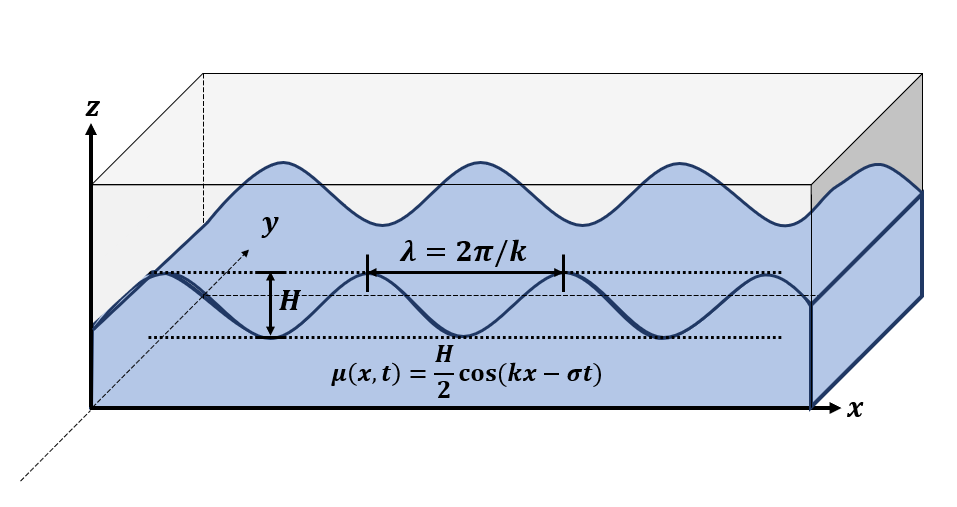
\includegraphics[width=10cm, trim={0 1.8cm 0 1.5cm}, clip]{Water_Tank(Illustrated).png}
\end{center}
\caption{조파 수조 모식도}
\label{Fig01}
\end{figure}
%해파를 만들때 현상을 재현하기 위한 환경을 조성하며 
조파기는 조파 수조에서 파를 생성하는 장치이다. 조파기는 판의 운동 방식에 따라 플랩형, 피스톤형, 플런저형 등이 있다. 연안 환경에서의 실험에 자주 사용되는 천해파를 생성하기에 용이한 피스톤형 조파기를 제작하였으며 파를 생성하는 조파판의 모든 요소가 일관적으로 수평 운동을 한다. 판의 수평 운동 범위를 스트로크라고 하며 $S_0$로 쓰도록 한다.
\begin{figure}[H]
    \begin{center}
        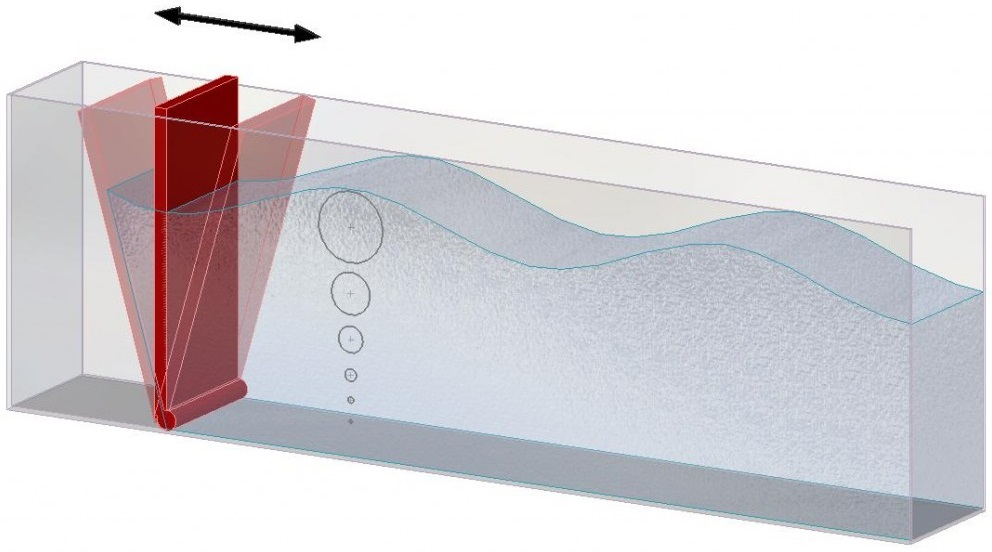
\includegraphics[height=3cm]{images/Wave_Maker(Flap).jpg}
        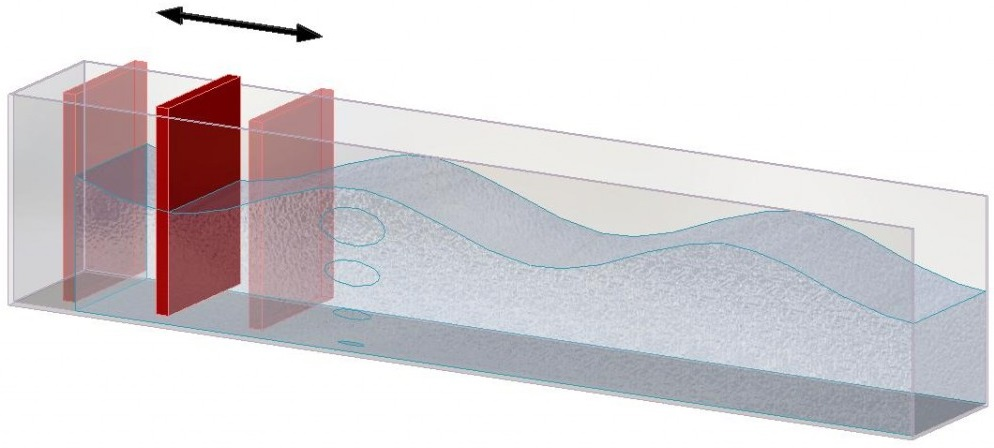
\includegraphics[height=3cm]{images/Wave_Maker(Piston).jpg}
    \end{center}
        \begin{tikzpicture} [remember picture, overlay]
            \node at (3.2, 1.0) {\scriptsize{(a) 플랩형}};
            \node at (9.0, 1.0) {\scriptsize{(b) 피스톤형}};
        \end{tikzpicture}
        \caption{다양한 종류의 2차원 조파기 - (a) 플랩형 (b) 피스톤형}
        \label{Experimnet_System} 
\end{figure}

\subsection{조파 이론 (wave maker theory)}

조파 이론은 여러 종류의 조파기가 발생하는 파도의 특성과 개형을 알아보는 것을 목표로 한다\cite{zhang2007deterministic,ojk2018}.
2차원 조파 수조에서 피스톤형 조파기가 발생시키는 파도는 여러 방정식을 통해 구할 수 있으며 보편적으로 속도 퍼텐셜 $\phi(x, y, z, t)$를 정의하고 이에 대한 라플라스 방정식과 여러 경계조건을 적용한다. 일반해는 다음과 같다.
\begin{equation} \label{eq:1}
{
\phi(x, z, t) = A\cosh{[k(h+z)]}\sin(kx-\sigma t) +
\cos(\sigma t){\sum_{n=1}^{\infty}} C_n e^{-k_3 x} \cos{[k_3 (z+h)]} 
}
\end{equation}

%$$\phi(x, z, t) = A\cosh{[k(h+z)]}\sin(kx-\sigma t) + $$
%$$\cos(\sigma t){\sum_{n=1}^{\infty}} C_n e^{-k_3 x} \cos{[k_3 (z+h)]}  $$

파동은 $x$방향으로 진행하며 $h$는 수심이고 $k$는 파수, $\sigma$는 각진동수이다. 그외의 문자는 상수이며 식 (\ref{eq:1})로부터 발생파의 변위 식을 다음과 같이 쓸 수 있다.
\begin{equation} \label{eq:2}
{
\mu(x, t) = {{1 \over g}{{\partial \phi} \over {\partial t}}|_{z=0} } = \frac{A \sigma}{g} \cosh(kh) \cos(kx-\sigma t) +
\sin(\sigma t) {\sum_{n=1}^{\infty}} \frac{\sigma C_n}{g} e^{-k_3 x} \cos(k_3 h)
}
\end{equation}

%$$\mu(x, t) = \frac{A \sigma}{g} \cosh(kh) \cos(kx-\sigma t) + $$
%$$\sin(\sigma t) {\sum_{n=1}^{\infty}} \frac{\sigma C_n}{g} e^{-k_3 x} cos(k_3 h) $$

식 (\ref{eq:1}), (\ref{eq:2}) 모두 첫 항은 진행파, 두 번째 항은 정상파에 대응된다. 정상파의 $k_3$은 진팽파의 분산관계식을 정상파 파수로 변환한 식에서 구할 수 있으며 $\sigma ^2 = -g k_3 \tan{k_3 h}$의 해이다. 하지만 제일 큰 해에 대해서 감쇠되는 비율 $\exp{(-k_{3}x)}$은 $x=2h$일 때 $0.04$, $x=3h$일 때 $0.009$ 수준으로 급감하며 본 연구에서는 수조 길이가 $6~\mathrm{m}$, 수심이 약 $15~\mathrm{cm}$ 수준이므로 정상파는 무시할 수 있다. 미분방정식의 각각의 고유함수에 대해 일차 근사를 적용하여 파고 $H$를 다음과 같이 표현할 수 있다.
\begin{equation} \label{eq:4}
H = \frac{4 S_0 \sinh{kh}}{\sinh{2kh}+2kh} \left(\sinh{k[z_d - h]} - \sinh{k[z_u - h]}\right)
\end{equation}

%$$H = \frac{4 S_0 \sin h{kh}}{\sin h{2kh}+2kh} (\sin h{k[z_d - h]} - \sin h{k[z_u - h]}) $$

$z_d$는 조파판 하단의 깊이, $z_u$는 조파판 상단의 깊이이며 본 연구의 경우 조파판이 수심 전체에 걸쳐 존재하므로 $z_d = h$, $z_u = 0$이고 파고와 파동 함수는 다음과 같다.
\begin{equation} \label{eq:5}
{
    \frac{H}{S_0}=\frac{4 (\sinh{kh})^{2}}{\sinh{2kh} + 2kh}
     = \frac{4 (\sinh{z})^{2}}{\sinh{2z} + 2z} ~(z=kh),~~
    \mu(x, t)=\frac{H}{2} \cos (kx -\sigma t)
}
\end{equation}

%$$\frac{H}{S_0}=\frac{4 \sinh ^2 k h}{\sinh k h+2 k h}, \mu(x, t)=\frac{H}{2} \cos (k x-\sigma t)$$

$S_0 ,~h$는 구조적인 값으로 조절 가능하며 파수 $k$와 각진동수 $\sigma$는 분산 관계식을 만족하므로 결론적으로 $\sigma$와 $S_0 , ~h$를 정하면 파가 결정된다. 조파판 또한 $\sin$형으로 움직이도록 경계조건으로 반영되었으며 판의 진동 변위는 다음과 같다.
\begin{equation} \label{eq:7}
{
    x = {{S_0}\over2} \sin{\sigma t}
}
\end{equation}

이는 심해파의 경우이다. 여러 경계조건과 근사를 위한 조건이 내포되어 있으며 간단히 $h/\lambda > 1/2$인 파를 의미한다. 천해파는 $h/\lambda < 1/20$이며 상대적으로 얕은 바다에서 생기며 파가 진행하면서 부서진다. 그렇기 때문에 이론적으로 파의 개형을 해석적으로 유도하기는 거의 불가능하며 대부분의 선행연구는 섭동이론을 적용하거나 2차까지 근사를 하는 등 비선형으로 방정식을 수치해석한다 \cite{society1993laboratory}. 

\subsection{소파 장치(wave absorber)}
파는 수조 내부에서 전달되며 진행파와 주변 장애물에 부딫혀 반사된 반사파가 중첩되어 정상파가 생성되고 오차의 주요 원인이 된다. 소파기는 반사파가 생기지 않도록 해주는 장치로 능동형 소파 장치(active wave absorber)\와 수동형 소파 장치(passive wave absorber)로 나뉜다\cite{ouellet1986survey}.

%\subsubsection{능동형 소파기}

능동형 소파 장치는 다른 조파기를 설치하여 벽에 입사하는 파를 완전히 상쇄시키는 파를 생성한다. 벽에 입사하는 파의 개형을 실시간으로 측정하여 이에 맞는 파를 발생시킬 수 있어야 하므로 측정과 파 발생 장치가 필요하며 고가의 장비이고 사용가능한 환경 및 구조가 제한되어 있다. 벽 부근에 다른 조파기를 설치하는 것이며 조파기가 자체적으로 운동을 제어하여 반사파를 상쇄시키도록 움직인다. '흡수 조파' 방식이라 불리며 조파판에서 파의 개형을 측정하여 반사파를 상쇄하는 파를 추가적으로 생성한다.

%\subsubsection{수동형 소파기(passive wave absorber)}

수동형 소파 장치는 추가적인 구조물을 설치하여 반사파의 에너지를 최소화한다. 능동형 소파 장치와 달리 아무리 최적화를 해도 항상 반사파가 존재하며 horsehair, crushed rock 등 여러 구조가 있다. 파를 효과적으로 소멸시키기 위해 다공성 판을 이용하며 공극률에 따른 반사계수 비교 등 다공성 구조 관련 선행 연구가 다수 진행되었고 이미 그 효율성이 입증되었다\cite{lim2014optimum,o2017methods}. 경사로를 이용하기도 하며 주로 3차원 조파 수조에서 파를 관찰하려는 영역이 아닌 다른 부분에서 최대한 상쇄시키기 위함이다. 경사로는 위로 볼록한 포물면을 띄는 경우가 제일 반사계수가 낮음이 밝혀졌다. 본 연구에서는 수동형 소파기를 사용한다.

\subsection{파고계(wave gauge)}

파고계는 파도의 높이(파고)를 재기 위한 측정 장치이다. 측정 방식에 따라 용량식, 저항식, 수압식, 초음파식 등여러 종류로 나뉘며 사용하는 장소의 규모, 정밀도에 따라 달라진다. 본 연구에서는 저항형 파고계를 사용하려 하였으나 제대로 측정이 되지 않았다. 물에 잠긴 와이어의 깊이에 따라서 전기전도도가 달라지고 저항이 바뀌는 점을 이용하여 전류값과 수심을 대응시키는 원리이지만 실험 결과 수심이 $20\mathrm{~cm}$가 바뀔 동안 전류가 $0.1\mathrm{~A}$ 바뀌었으며 이 값이 최소눈금이다. 전류 증폭을 시도해보았으나 회로가 버틸 수 있는 범위 내에서는 측정을 할 수 없으며 결국 부표를 띄우고 영상을 찍어 파도의 파고 데이터를 얻어내는 방식을 채택하였다.

\subsection{Froude 상사 법칙}
모형실험을 하는 경우 축척이 달라지면 물리적 특성이 바뀐다. 무차원 수가 보존되어야 한다는 원리가 Froude 상사 법칙이며 보존되는 무차원 수를 Froude 수라고 한다.\cite{briggs2013basics, chakrabarti1994offshore} 이외에도 Reynolds 수, Prandtl 수 등이 보존되기도 하나 본 실험의 경우 파의 진행에 초점을 맞추기 때문에 Froude 수가 보존되는 경우를 생각한다. 이는 다음과 같이 정의된다.
\begin{equation}
    Fr = \frac{V}{\sqrt{gL}}
\end{equation}

$V$는 운동의 주체(파도; 물, 배, 비행기 등)의 속도이며 $g$는 중력가속도, $L$은 계의 특성길이이다. 수조와 바다에 대한 Froude 수가 같아야 하며 두 계 모두 움직이는 주체는 파도이기 때문에 분산 관계식을 이용하여 새롭게 쓸 수 있다.

\begin{equation}
    Fr = \sqrt{\frac{\tanh{kh}}{kL}}
\end{equation}

특성 길이는 단면이 직사각형인 수조의 경우 $L = {2ab}/{(a+b)}$임이 알려져 있으며 $a$는 수조의 폭, $b$는 수조 내 물의 수심이다. 바다의 경우 이를 근사적으로 $2h$로 생각할 수 있다 ($h$는 바다의 수심이다). $a=30\mathrm{~cm}, b=15\mathrm{~cm}$를 대입하면 관계식에 의해 모형 실험의 경우 천해파는 $\omega \sim \pi$, 심해파는 $\omega \sim 4\pi$ 정도 되어야 한다 (단, 각각 심해파, 천해파의 경계값인 $h/\lambda = 1/2, 1/20$에 대한 값이다).

% \begin{quote}
%     \[f(z_i) = \frac{\tanh{z_i}}{z_i},~  z_i = k_i h_i\]

%     \begin{multicols}{2}

%     계 1: 수조
%     \[{Fr_1}^{2} = \frac{a+b}{2ab} \frac{\tanh{k_1 b}}{k_1} = \frac{3}{4} f(z_{1})\]

%     \columnbreak
    
%     계 2: 깊은 바다
%     \[{Fr_2}^{2} = \frac{1}{2h_2} \frac{\tanh{k_2 h_2}}{k_2} = \frac{1}{2} f(z_{2})\]
%     \end{multicols}

% \end{quote}

% \begin{equation}
%     \therefore \frac{3}{2}f(z_1 ) = f(z_2 )
% \end{equation}



\section{2차원 조파 수조 제작 결과}

\subsection{조파 수조 개관}

\begin{figure}[H]
        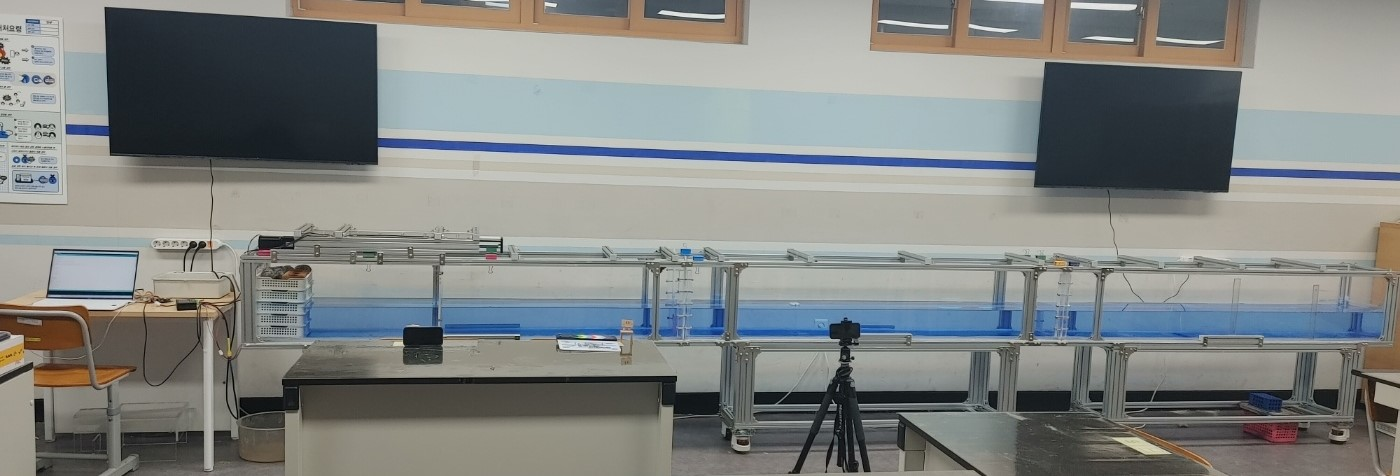
\includegraphics[width=\textwidth]{images/Experiment_System_Crop}
        \captionof{figure}{완성된 조파수조의 모습}
        
 %       \label{Experimnet_System} 
        \begin{tikzpicture} [remember picture, overlay, anchor=north west]
            \node [draw=yellow, text=yellow] (TV1) at (2.5, 5.8) {\scriptsize{TV1}};
            \node [draw=yellow, text=yellow] (TV2) at (14, 5.5) {\scriptsize{TV2}};
            \node [draw=yellow, text=yellow] (computer) at (1.0, 4) {\scriptsize{computer}};
            \node [draw=yellow, text=yellow] at (4.6, 2.6) {\scriptsize{camera1}};
            \node [draw=yellow, text=yellow] at (9.5, 2.5) {\scriptsize{camera2}}; 
        \end{tikzpicture}
        %\captionof{figure}{\scriptsize 완성된 조파 수조의 모습} %\\[0.5em]\
\end{figure}
 
제작한 작품은 `2차원 조파 수조'로 명명하였다. 조파 수조를 이용하여 실험할 때 제대로 진행되려면 조파기, 소파기, 파고계, 해안 경사로 등이 제 역할을 해줘야 한다. 따라서 각 부분은 실험 목적에 따라 조립과 분해가 가능하도록 따로 제작하였고 조파 수조의 특징을 나열하면 다음과 같다.

\begin{itemize}
    \item 규격은 폭 $300~\mathrm{mm}$, 높이 $400~\mathrm{mm}$, 총 길이 $6,000~\mathrm{mm}$이다. 길이 $2,000~\mathrm{mm}$의 모듈 3개를 이어붙였으며 추가로 제작하여 연결하면 길이 연장이 가능하다.
    \item 조파기는 리니어 엑츄레이터를 이용하여 구동부를 제작하였고 틴지 보드를 기반으로 하여 스텝 모터를 구동하는 제어부를 제작하였다.
    \item 현재 조파기로 규칙파를 생성하는 코드를 완성하여 검증했으며 코드가 정교화되면 다양한 주기, 파장, 파고의 규칙파를 생성할 수 있다. 
    \item 코드를 업그레이드하여 쓰나미 등의 불규칙파를 정교하게 제어할 수 있도록 할 것이다.
    \item 경사로는 교각 위에 아크릴 판을 장치하였고 길이와 기울기를 변화시킬 수 있으며 탈부착 가능하다.
    \item 파고계는 물에 잘 뜨는 재질로 제작하여 동영상 분석을 통해 파고를 파악하고 있으며, 이후 센서를 부착하여 정밀한 파고를 측정하도록 개선할 예정이다.
\end{itemize}

\subsection{수조 모듈 구성 및 연결 방법}
수조는 길이 $2,000~\mathrm{mm}$, 폭 $300~\mathrm{mm}$, 높이 $400~\mathrm{mm}$인 수조 모듈로 구성되어 있으며 3개를 연결하여 총 길이 $6,000~\mathrm{mm}$이다. 모듈의 기본 프레임은 알루미늄 프로파일 3030 시리즈이며 두께 $5~\mathrm{mm}$의 아크릴 판을 이용하여 물이 담기는 수조를 제작하였다. 수조의 모서리 부분은 인접한 두 아크릴 판을 아크릴 접착제로 붙였으며 실리콘으로 방수 처리를 하였다. 수준기로 수평이 맞는지 여러 방향에서 확인하여 모듈 3개가 일직선을 이루도록 해야 한다. 모듈 사이의 연결부는 실리콘 패드를 잘라 사이에 끼웠고 아크릴 판의 옆, 아래에는 볼트가 들어갈만한 크기의 아크릴 조인트를 부착하여 볼트와 너트로 밀착하였다. 물이 새지 않도록 정교하게 연결해야 하며 실리콘으로 방수 처리를 하여 총 길이 $6,000~\mathrm{mm}$의 수조를 완성하였다. 규격에 맞는 수조 모듈을 제작하여 삽입하면 길이 연장이 가능하다.

\begin{figure}[H]
	\begin{center}
		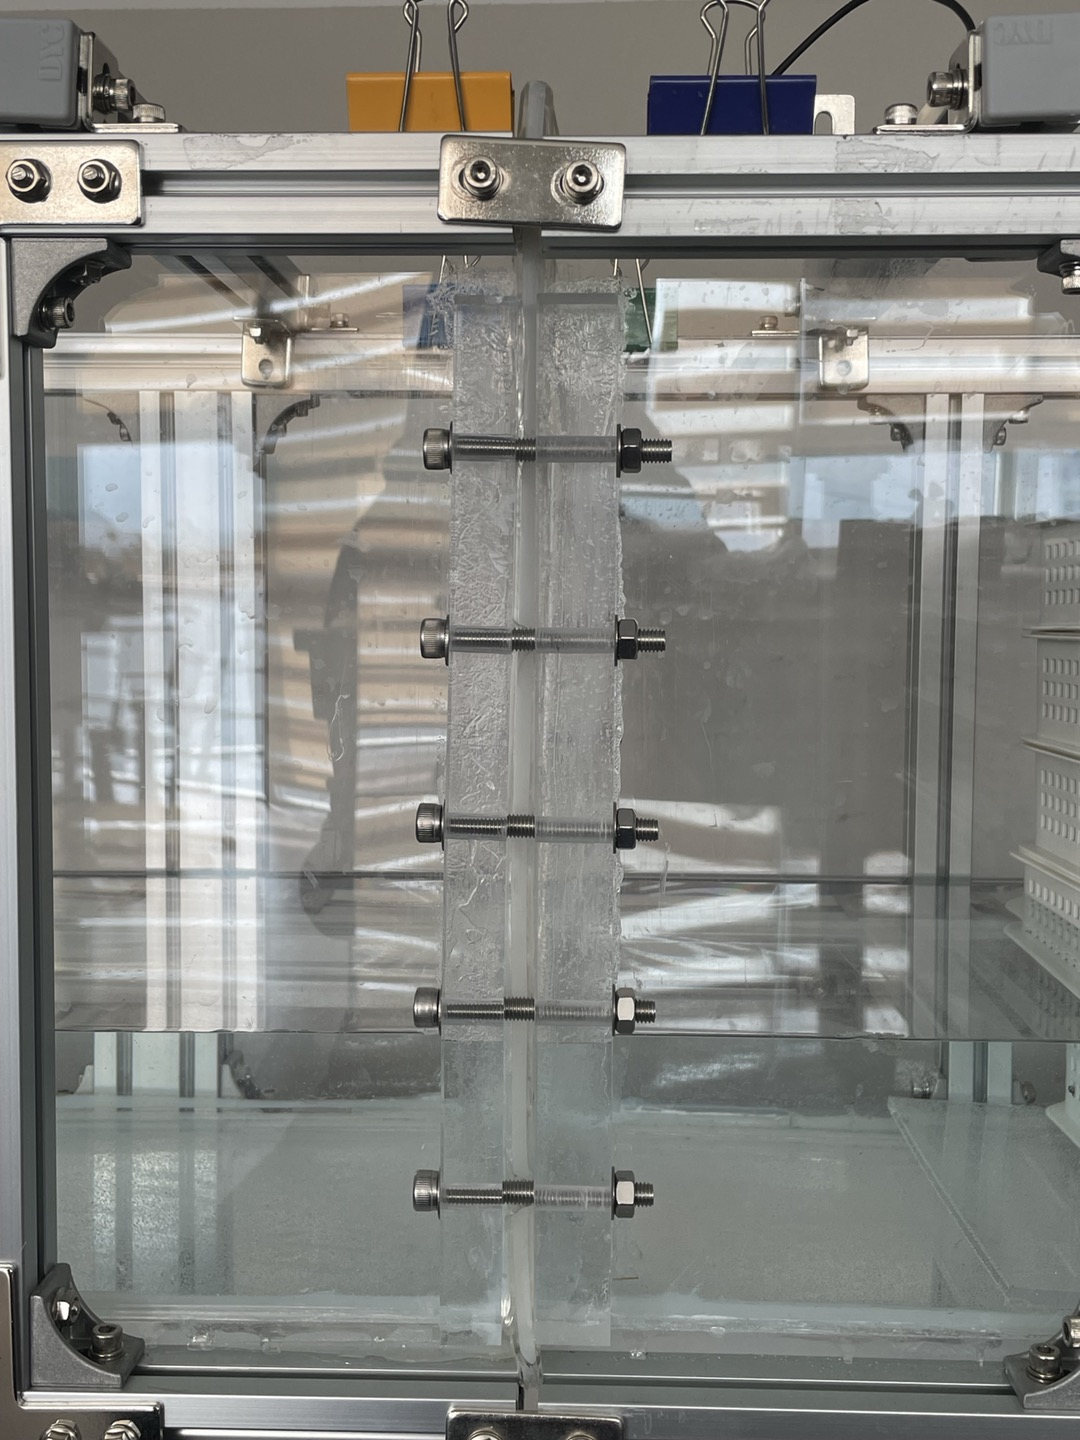
\includegraphics[width=0.3\textwidth]{images/magam1.jpg}
		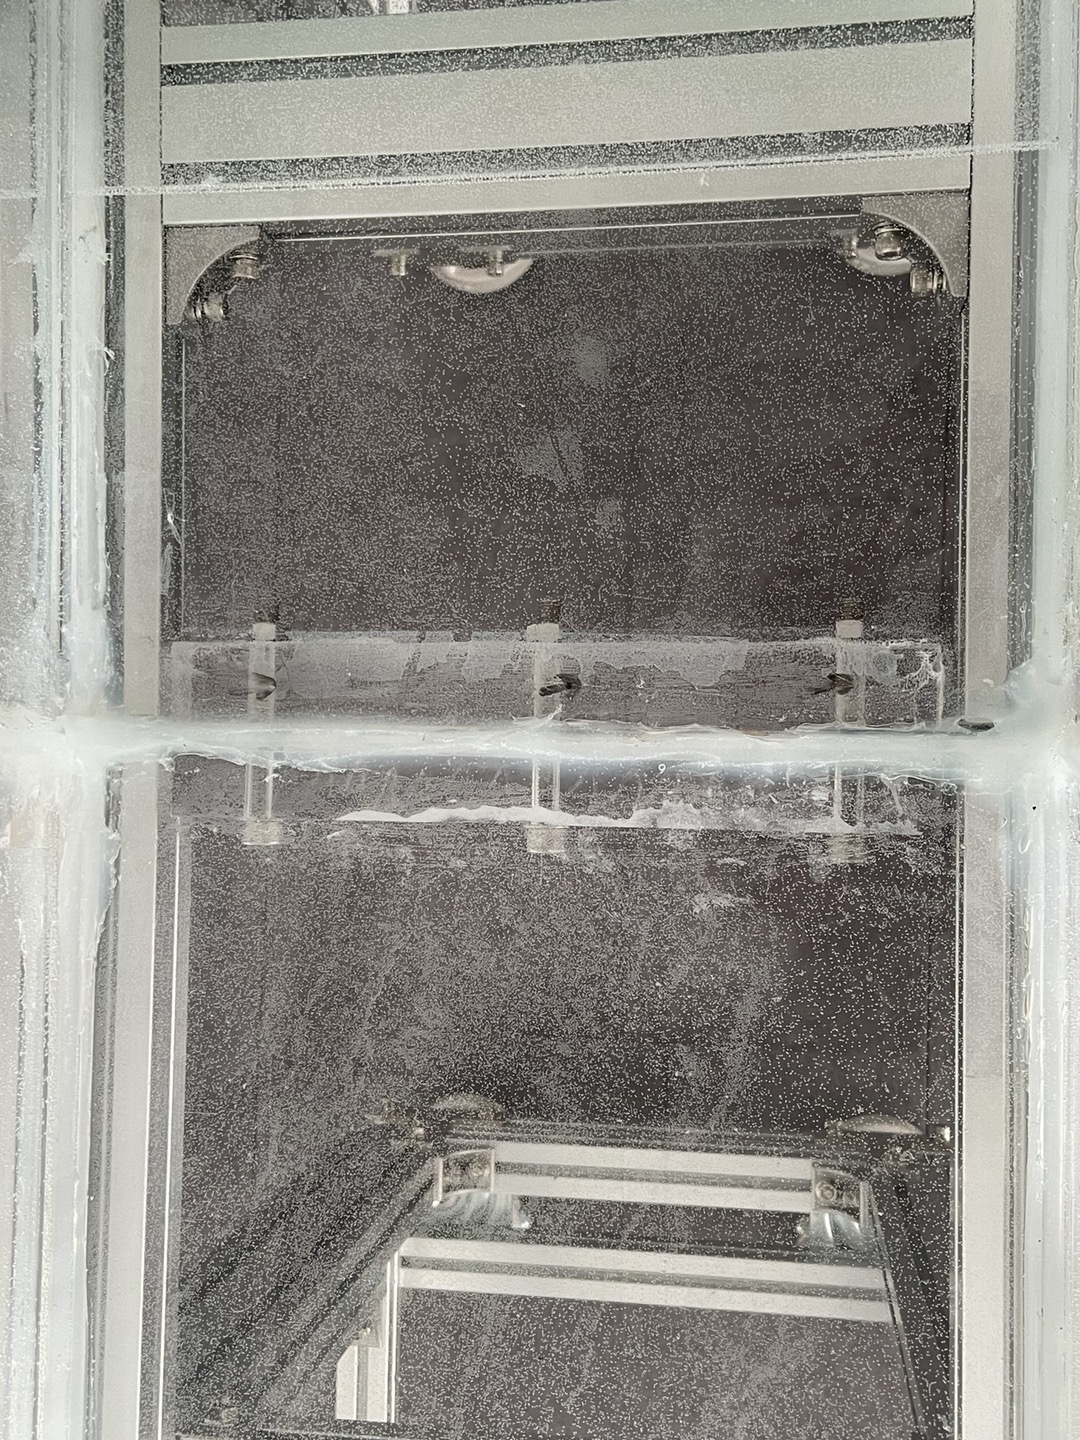
\includegraphics[width=0.3\textwidth]{images/magam2.jpg}
		\caption{수조 연결부의 모습}
		\label{Waveabsorber}
	\end{center}
\end{figure}

\subsection{소파 장치}
해파의 전파 중 벽이나 장애물에 부딫히면 반사파가 발생하며 수조는 양 끝이 막힌 구조로 조파기에서 기원한 해파와 반사파가 간섭을 일으키고 정상파가 생성되어 주요 오차 요인이 된다. 조파판이 식 (\ref{eq:7})\을 따라 움직이면서 판의 뒷부분으로 진행하는 파를 생성하며 판의 앞부분으로 진행하는 파는 수조의 말단에서 정상파를 형성하지만 $x/h > 20$이므로 (수심은 $30\mathrm{~cm}$ 미만이다) 충분히 무시할 수 있다. 이는 수조가 무한히 길다고 가정한 상황이며 실제로는 반사파가 생길 수 있다. 판의 뒷부분으로 진행하는 파는 좁은 공간에서 계속 중첩되며 판에 계속 부하를 가하기 때문에 소파 장치가 필요하다.

\begin{figure}[H]
	\begin{center}
		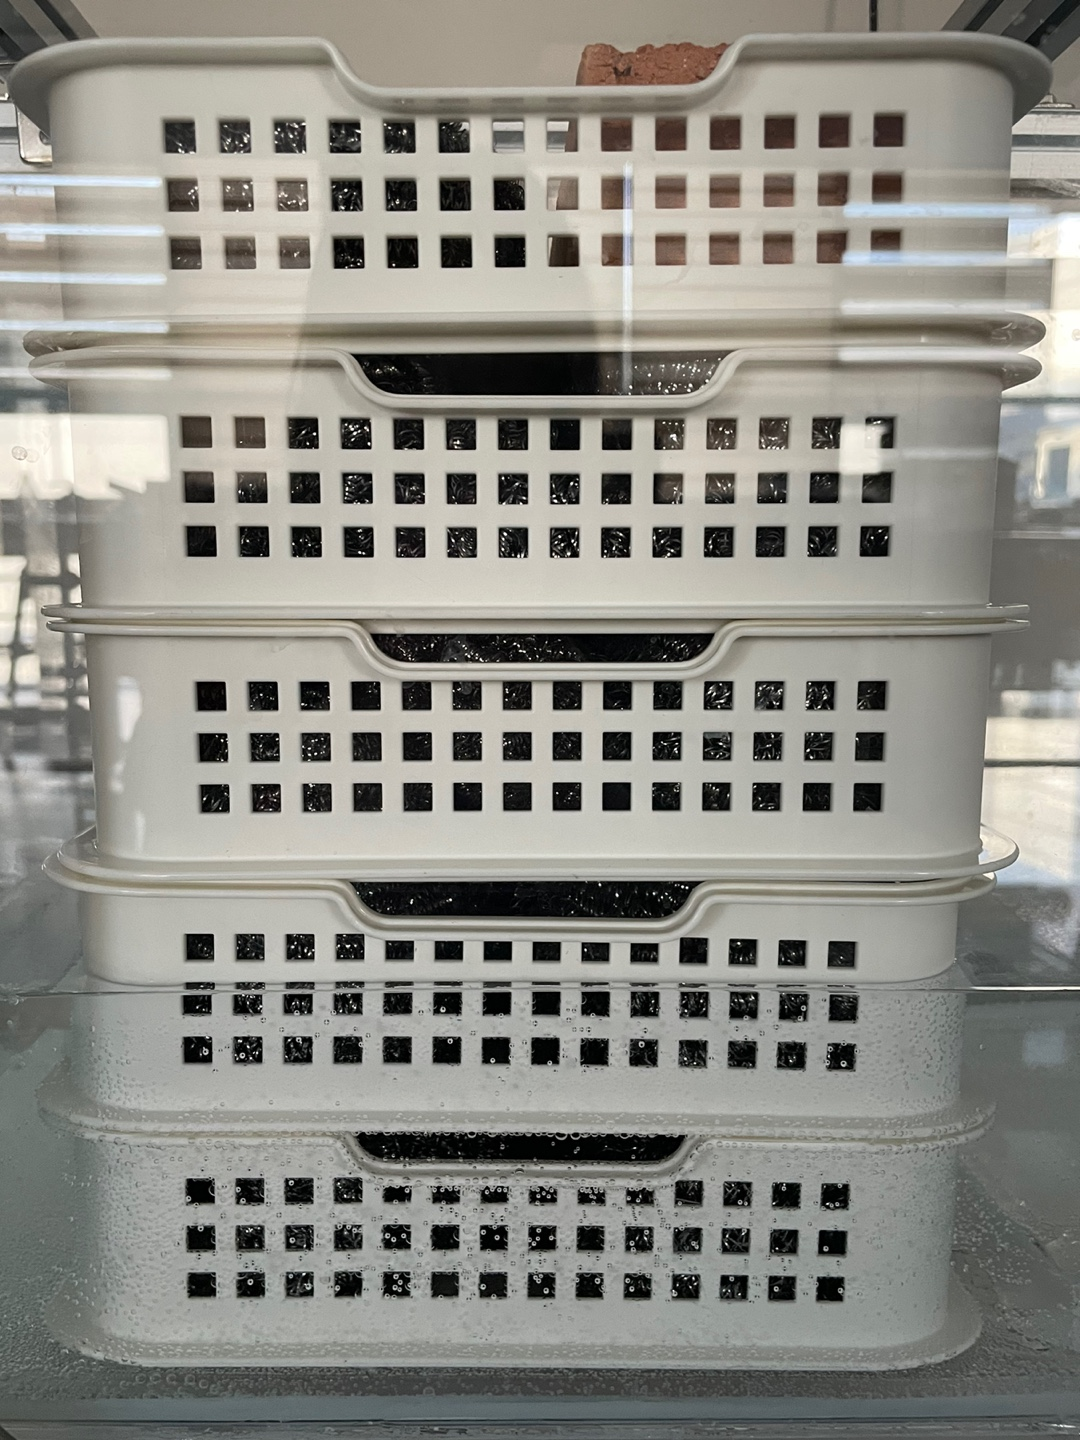
\includegraphics[width=0.3\textwidth]{images/sopagi1.jpg}
		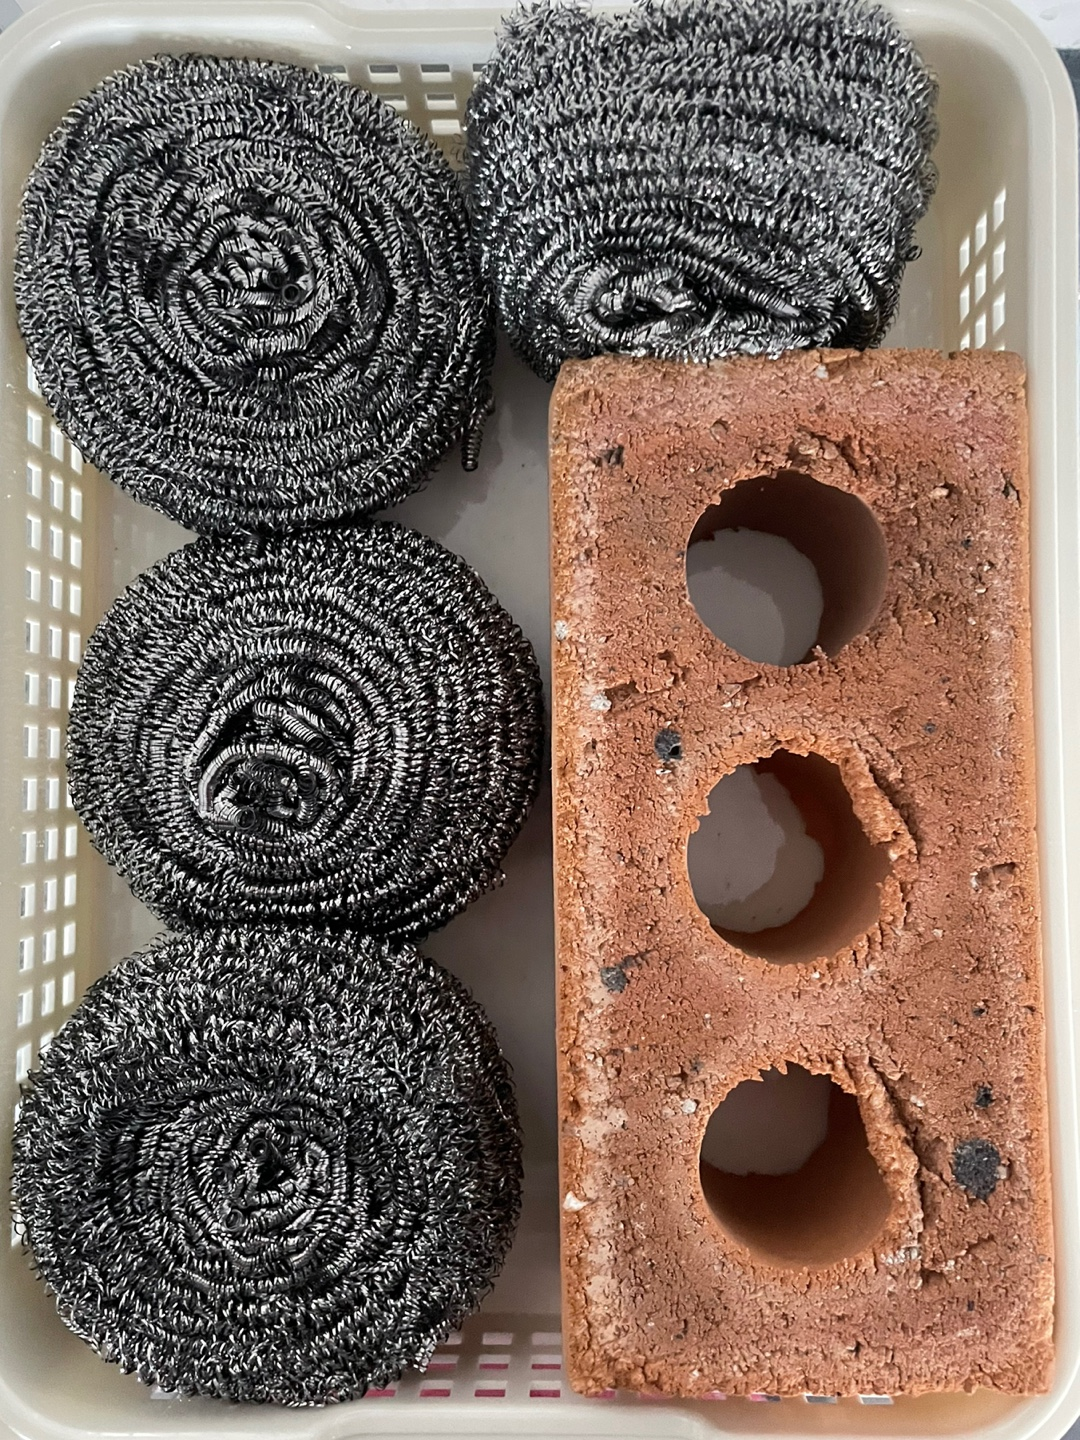
\includegraphics[width=0.3\textwidth]{images/sopagi2.jpg}
		\caption{플라스틱 바구니와 수세미를 이용해 만든 소파 장치}
		\label{Waveabsorber}
	\end{center}
\end{figure}

소파 장치는 해파의 에너지를 흡수할 수 있는 다공질의 구조가 소파 성능이 좋다는 선행 연구 결과에 착안하여 구멍이 뚫린 플라스틱 바구니에 철 수세미를 넣어 제작하였다\cite{lim2014optimum, o2017methods}. 플라스틱 바구니에 철수세미를 최대한 밀착하여 집어넣어 다공성 구조를 형성해주었고 물에 뜨기 때문에 가장 윗 칸에 벽돌을 올렸다. 2개를 제작하여 조파 수조의 양 말단에 설치하였다.

\subsection{연안 모형 (해안 경사)}

먼 바다에서 해안으로 올수록 수심이 얕아지고 지면의 영향이 증가하면서 해파는 심해파, 천이파, 천해파로 변한다. 파가 굴절되고 속도가 느려지면서 쇄파 현상이 발생한다. 해파는 연안의 모양에 따라 서로 다른 모양을 띄며 여러 연안 모형에 대한 실험 환경이 필요하다. 본 연구의 연안 모형은 목적에 맡게 바꿀 수 있고 탈부착이 가능하다. 일정한 너비의 아크릴 판을 수조 바닥에 부착했고 육지는 알루미늄 프로파일 교각으로 높이 차를 주었으며 해안 경사 바닥을 안정적으로 지지할 수 있다. 실제 우리나라 주변의 바다는 동해, 황해, 남해의 전형적인 해안 경사가 다르고 해파의 영향으로 상당히 가변적이기 때문에 다양한 기울기의 해안 경사를 가질 수 있도록 다양한 길이의 교각을 준비하였다. 현재 설치한 경사로는 높이 $200\mathrm{~mm}$, 길이 $2,000\mathrm{~mm}$로 기울기가 $1/10$ 이다. 

\begin{figure}[htbp]
	\begin{center}
		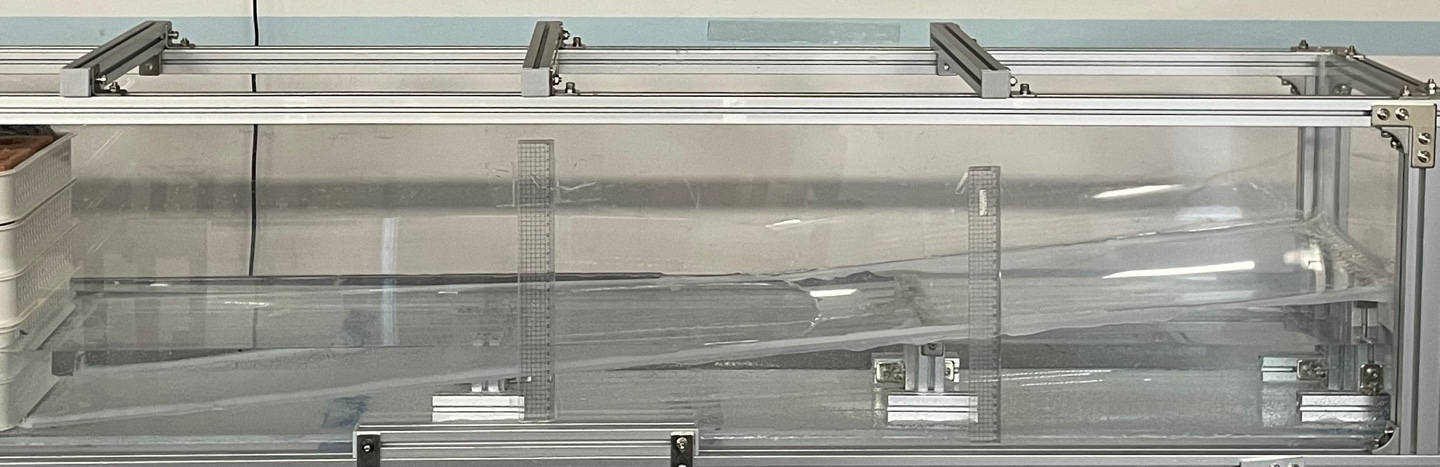
\includegraphics[width=0.8\textwidth]{images/slope.jpg}
		\caption{설치한 연안 모형}
		\label{Slope}
	\end{center}
\end{figure}


\subsection{방파제 모형}
현재 해안 모형은 경사로이지만 육지 공간을 넓히면 구조물을 설치할 수 있다. 파력 발전 시설을 두어 여러 발전 시스템의 효율 비교 및 최적화 연구를 진행할 수도 있고 구조물의 내구성 실험도 가능하다. 나아가 경사로의 기울기도 변화시켜 여러 환경에서 다양한 실험을 진행할 수 있으며 추후에 판을 덧대는 것이 아닌 일체형으로 만들어 관리에 용이하도록 할 예정이다.

\begin{figure}[H]
    \centering
    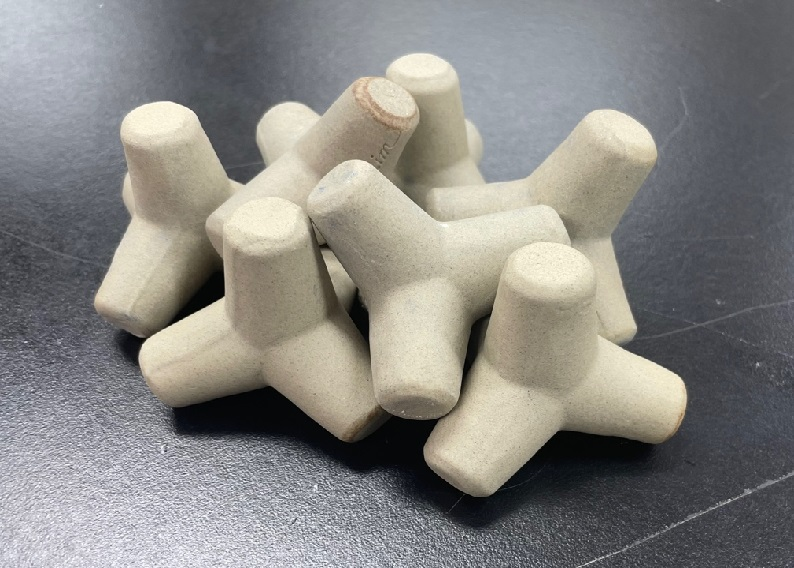
\includegraphics[height=5.5cm]{images/Breakwater.jpg}
    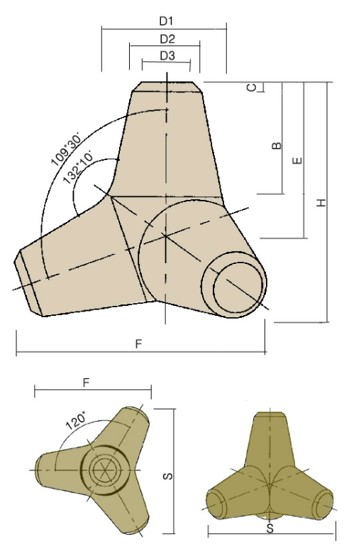
\includegraphics[height=5.5cm]{images/Breakwater(Illustrated).jpg}
    \caption{방파제 모형(왼쪽)과 규격(오른쪽)}
    \label{Braekwater}
\end{figure}

본교에는 규격 $D3=1.2\mathrm{~cm}, D2=1.7\mathrm{~cm}, S=5.3\mathrm{~cm}, F=5\mathrm{~cm}$의 방파제 모형이 있으며 여러 연구에서 이를 이용할 수 있다. Gurer의 구조, Fabiao의 구조 등 다양한 조적 구조가 있으며 구조의 종류 및 스케일에 대한 방파 효과를 비교할 수도 있다 \cite{article}.

\subsection{조파기}

조파기는 구동부와 제어부로 나뉜다. 구동부는 조파기의 기계적인 부분으로 리니어 액츄에이터와 이를 고정할 여러 부품으로 구성되어 있다. 제어부는 모터의 회전을 제어하는 부분으로 모터 드라이버와 틴지 보드 3.2(Teensy Board)로 구성되어 있다.

%\subsubsection{구동부}

구동부는 $80\mathrm{~cm}$ 길이의 리니어 액츄에이터(linear actuator)를 메인 부품으로 하여 알루미늄 프로파일 프레임을 만들었다. 리니어 액츄에이터의 운동부에는 아크릴 재질의 조파판을 장착하였고 수조 내부에 들어가도록 구동부를 수조 위에 장치하였다. 아크릴 판의 규격은 $280\mathrm{~mm} ~\times~ 295\mathrm{~mm} ~\times~5\mathrm{~mm}$로 수조 내부 공간에 딱 들어맞으며 최대한 밀착되어야 정교한 파를 생성할 수 있다. 조파판이 리니어 액츄에이터의 이동부에 붙어 수조 내부를 수평적으로 이동하며 물을 밀어내고 파를 생성한다. 액츄에이터는 FUYU 사의 FSK80 시리즈 제품으로 가동범위(stroke)는 $80\mathrm{~cm}$이고 최대 힘 $40\mathrm{~N}$, 최대 속력 $23\mathrm{~cm/s}$을 낼 수 있다(표 \ref{Specification of Linear Actuator}).

% \begin{figure}[H]
%     \begin{minipage}[t]{.3\linewidth}
%     \begin{center}
%         \scalebox{-1}[1]{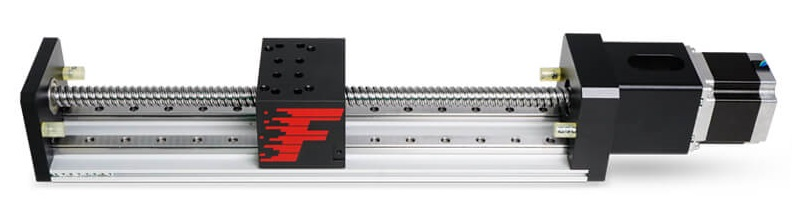
\includegraphics[width = 3cm]{images/Linear_Actuator.jpg}}
%         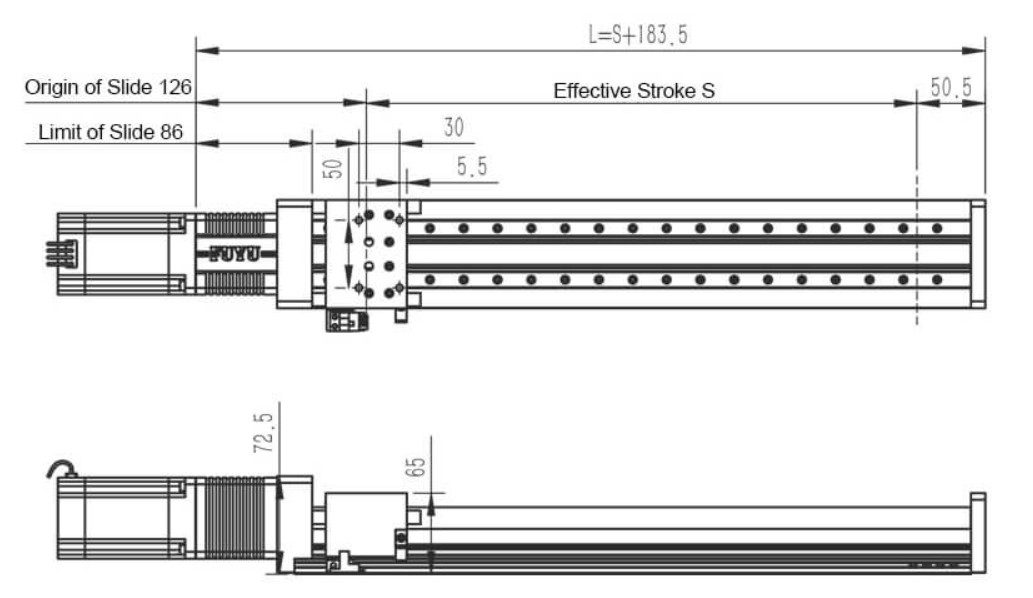
\includegraphics[width = 3cm]{images/Linear_Actuator(Design).jpg}
%     \end{center}
%         \begin{tikzpicture} [remember picture, overlay]
%         \node at (2.0, 11.0) {(a)};
%         \node at (2.0, 7.6) {(b)}; %1.1
%         \end{tikzpicture}	
%         %\caption{Linear actuator - (a) \textit{FSK80} series (b) Design}
%         \caption{(a) FUYU사의 FSK80 시리즈 리니어 액츄에이터, (b) 제원}
%         \label{linear actuator}
%     \centering
%   \end{minipage}\hfill
  
%   \begin{minipage}[t]{.6\linewidth}
%     \centering
%     \captionsetup{justification=centering}
%     \caption{리니어 액츄에이터의 스펙}
%     \begin{tabular}{l|l}
%         \hline
%         guide width $(\mathrm{mm})$                       & 80                                     \\
%         repeat position accuracy $(\mathrm{mm})$          & $\pm$0.02                                 \\
%         motor                                  & stepper 60102                          \\
%         % rail model                             & dual rail W12 $\times$ H8              \\
%         % ball screw model                       & 16                                     \\
%         \textbf{stroke $(\mathrm{mm})$}                  & \textbf{50 - 1000}                                    \\
%         pitch                                  & 10                                     \\
%         \textbf{horizontal full payload speed $(\mathrm{mm/s})$}   & \textbf{230}                                    \\
%         vertical full payload speed $(\mathrm{mm/s})$     & 60                                     \\
%         side mounting payload speed $(\mathrm{mm/s})$     & 210                                    \\
%         \textbf{rated horizontal payload $(\mathrm{kg})$}          & \textbf{40}                                     \\
%         rated vertical payload $(\mathrm{kg})$            & 20                                     \\
%         rated side mounting payload $(\mathrm{kg})$       & 15                                     \\
%         noisy without payload $(\mathrm{db})$             & 79                                     \\
%         rated payload noisy $(\mathrm{db})$               & 70                                     \\
%         \textbf{acceleration } $(\mathrm{mm/s}^{2})$   & \textbf{500}                                    \\ \hline
%     \end{tabular}%
%     \label{Specification of Linear Actuator}
%   \end{minipage}
% \end{figure}

%%%%%%%%%%%%%%%%%%%%%%%%%%%%%%%%%%%%%%%%%%%%%%%%%%%%%%%%%%%%%%%%%%%%%%%%%%%%%
% \begin{figure}[H]
%     \begin{center}
%         \scalebox{-1}[1]{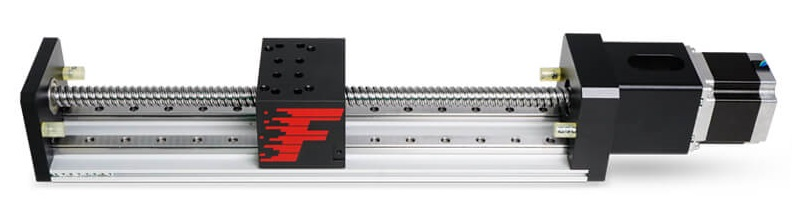
\includegraphics[width = 0.7\linewidth]{images/Linear_Actuator.jpg}}
%         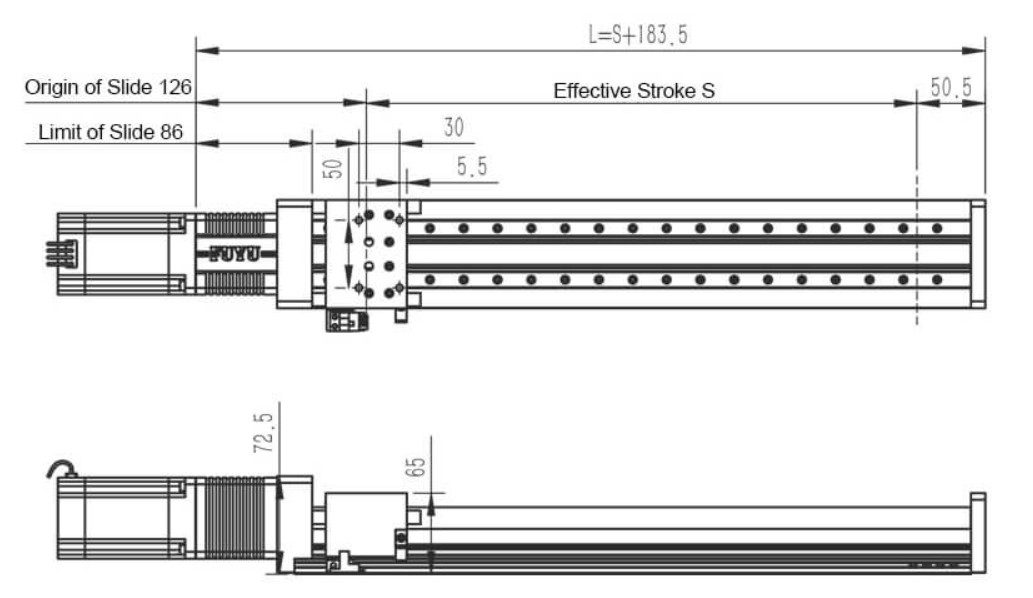
\includegraphics[width = 12cm]{images/Linear_Actuator(Design).jpg}
%     \end{center}
%         \begin{tikzpicture} [remember picture, overlay]
%         \node at (2.0, 11.0) {(a)};
%         \node at (2.0, 7.6) {(b)}; %1.1
%         \end{tikzpicture}	
%         %\caption{Linear actuator - (a) \textit{FSK80} series (b) Design}
%         \caption{(a) FUYU사의 FSK80 시리즈 리니어 액츄에이터, (b) 제원}
%         \label{linear actuator}
% \end{figure}
%%%%%%%%%%%%%%%%%%%%%%%%%%%%%%%%%%%%%%%%%%%%%%%%%%%%%%%%%%%%%%%%%%%%%%%%%%%%

% \begin{figure}[H]
%     \centering
%     \captionsetup{justification=centering}
%     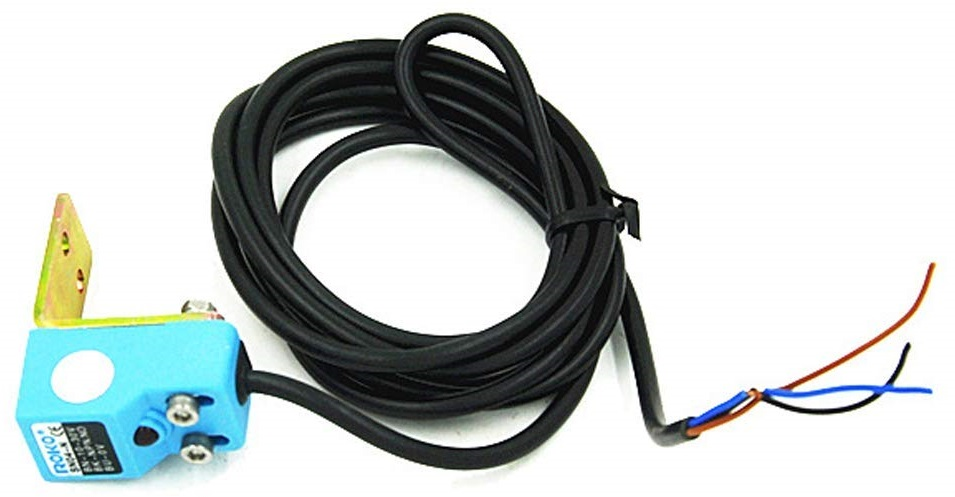
\includegraphics[width = 6cm]{images/Limit_Switch.jpg}
%     \caption{Limit Switch}
%     \label{limit switch}
% \end{figure}

% \begin{figure}
%     \centering
%     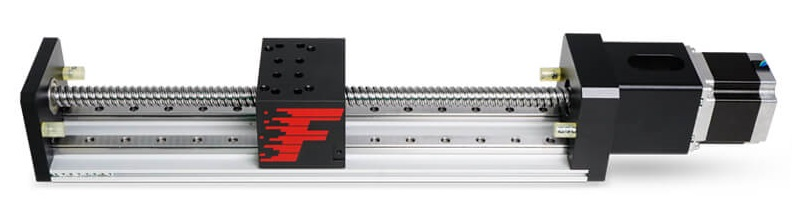
\includegraphics[width=0.5\textwidth]{images/Linear_Actuator.jpg}
%     \caption{FUYU사의 FSK80 시리즈 리니어 액츄에이터}
%     \label{Linear Actuator}
% \end{figure}

\begin{figure}[H]
    \begin{minipage}[b]{.45\linewidth}
        \centering
        \scalebox{-1}[1]{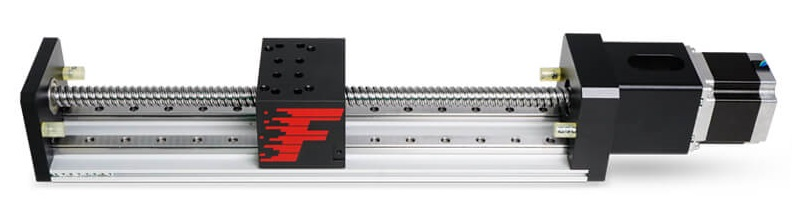
\includegraphics[width = 0.7\linewidth]{images/Linear_Actuator.jpg}}
        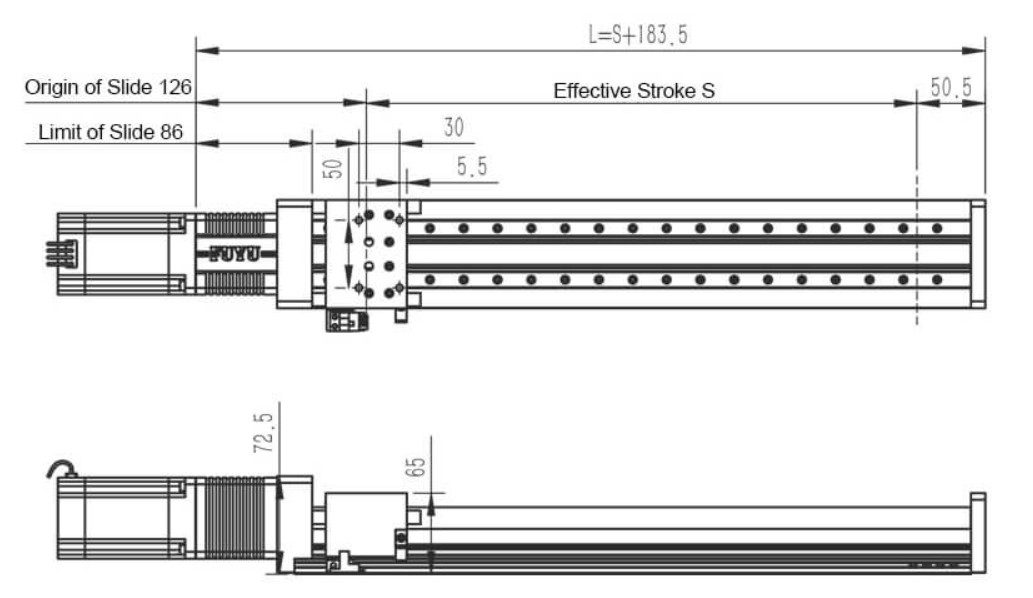
\includegraphics[width = 0.7\linewidth]{images/Linear_Actuator(Design).jpg}
        \captionof{figure}{FSK80 시리즈 리니어 액츄에이터}
        % \label{linear actuator}
    \end{minipage}\hfill
    \begin{minipage}[b]{.45\linewidth}
        \resizebox{\columnwidth}{!}{
        \begin{tabular}{l|l}
            \hline
            guide width $(\mathrm{mm})$                       & 80                                     \\
            repeat position accuracy $(\mathrm{mm})$          & $\pm$0.02                                 \\
            motor                                  & stepper 60102                          \\
            % rail model                             & dual rail W12 $\times$ H8              \\
            % ball screw model                       & 16                                     \\
            \textbf{stroke $(\mathrm{mm})$}                  & \textbf{50 - 1000}                                    \\
            pitch                                  & 10                                     \\
            \textbf{horizontal full payload speed $(\mathrm{mm/s})$}   & \textbf{230}                                    \\
            vertical full payload speed $(\mathrm{mm/s})$     & 60                                     \\
            side mounting payload speed $(\mathrm{mm/s})$     & 210                                    \\
            \textbf{rated horizontal payload $(\mathrm{kg})$}          & \textbf{40}                                     \\
            rated vertical payload $(\mathrm{kg})$            & 20                                     \\
            rated side mounting payload $(\mathrm{kg})$       & 15                                     \\
            noisy without payload $(\mathrm{db})$             & 79                                     \\
            rated payload noisy $(\mathrm{db})$               & 70                                     \\
            \textbf{acceleration } $(\mathrm{mm/s}^{2})$   & \textbf{500}                                    \\ \hline
        \end{tabular}}%
        \captionof{table}{리니어 액츄에이터 스펙}
        \label{Specification of Linear Actuator}
    \end{minipage}
\end{figure}

% \begin{table}[H]
%     \centering
%     \captionsetup{justification=centering}
%     \caption{리니어 액츄에이터의 스펙}
%     \begin{tabular}{l|l}
%         \hline
%         guide width $(\mathrm{mm})$                       & 80                                     \\
%         repeat position accuracy $(\mathrm{mm})$          & $\pm$0.02                                 \\
%         motor                                  & stepper 60102                          \\
%         % rail model                             & dual rail W12 $\times$ H8              \\
%         % ball screw model                       & 16                                     \\
%         \textbf{stroke $(\mathrm{mm})$}                  & \textbf{50 - 1000}                                    \\
%         pitch                                  & 10                                     \\
%         \textbf{horizontal full payload speed $(\mathrm{mm/s})$}   & \textbf{230}                                    \\
%         vertical full payload speed $(\mathrm{mm/s})$     & 60                                     \\
%         side mounting payload speed $(\mathrm{mm/s})$     & 210                                    \\
%         \textbf{rated horizontal payload $(\mathrm{kg})$}          & \textbf{40}                                     \\
%         rated vertical payload $(\mathrm{kg})$            & 20                                     \\
%         rated side mounting payload $(\mathrm{kg})$       & 15                                     \\
%         noisy without payload $(\mathrm{db})$             & 79                                     \\
%         rated payload noisy $(\mathrm{db})$               & 70                                     \\
%         \textbf{acceleration } $(\mathrm{mm/s}^{2})$   & \textbf{500}                                    \\ \hline
%     \end{tabular}%
%     \label{Specification of Linear Actuator}
% \end{table}


\begin{figure}[H]
    \centering
        \includegraphics[width=0.8\textwidth]{images/jopagi.jpg} 
    \caption{피스톤형 조파기의 구동부 모습}
    \label{wavemaker-photo}
\end{figure}
%%%%%%%%%%%%%%%%%%%%%%%%%%%%%%%%%%%%%%%%%%%%%%%%%%%%%%%%%%%%%%%%%%%%%%%%%

% \begin{figure}[H]
% 	\begin{center}
% 		\includegraphics[width=.7\textwidth]{jopagi.jpg}
% 		\caption{완성된 피스톤형 조파기의 모습}
% 		\label{Wavetank}
% 	\end{center}
% \end{figure}

%\subsubsection{회로부}

제어부는 틴지 보드 3.2와 DRV8825, Microstep Driver(ST-M5045), $48\mathrm{~V}$ SMPS(Switching Mode Power Supply)로 구성되어 있다. DRV8825와 ST-M5045는 모터 드라이버로 모터의 구동을 제어한다. DRV8825는 pcb 보드에 장착하는 스텝 모터 드라이버이며 ST-M5045 외장형 스텝 모터 드라이버이다. SMPS는 변압기로 공급 전압을 높여주며 $36, ~48~\mathrm{V}$ 변압기로 갈아끼울 수 있다. 틴지 보드 3.2는 메인 CPU 역할을 하며 코드를 실행한다.

\begin{figure}[H]
  \begin{minipage}[b]{.5\linewidth}
    \centering
    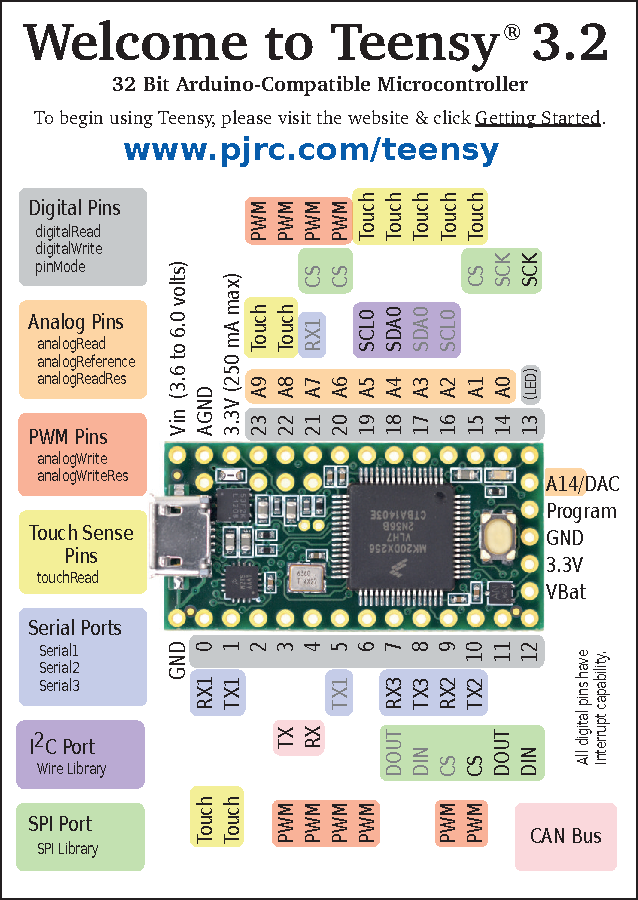
\includegraphics[width=0.45\linewidth]{images/Teensy3.2 - 1.pdf}
    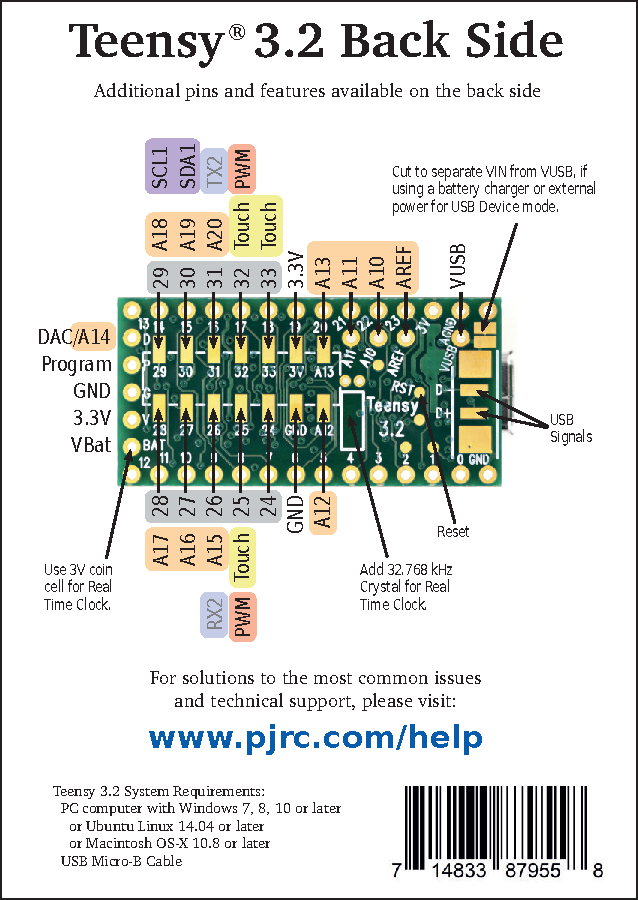
\includegraphics[width=0.45\linewidth]{images/Teensy3.2 - 2.pdf}
    \captionof{figure}{틴지 보드의 핀 맵(pin map)}% \caption{Figure caption}
  \end{minipage}\hfill
  \begin{minipage}[b]{.5\linewidth}
    \centering
    \resizebox{\columnwidth}{!}{
        \begin{tabular}{l}
            \hline
            ARM Cortex-M4 at 72 MHz\\
            256K Flash, 64K RAM, 2K EEPROM\\
            USB device 12 Mbit/sec\\
            34 digital input/output pins, 12 PWM output pins\\
            21 analog input pins, 1 analog output pin, 12 capacitive sense pins\\
            3 serial, 1 SPI, 2 I2C ports\\
            1 I2S/TDM digital audio port\\
            1 CAN bus\\
            16 general purpose DMA channels\\
            RTC for date/time\\
            \hline
        \end{tabular}
    }
    \captionof{table}{틴지 보드의 스펙}
    \label{Specification of Teensy Board}
  \end{minipage}
\end{figure}

\begin{figure}[H]
	\begin{center}
		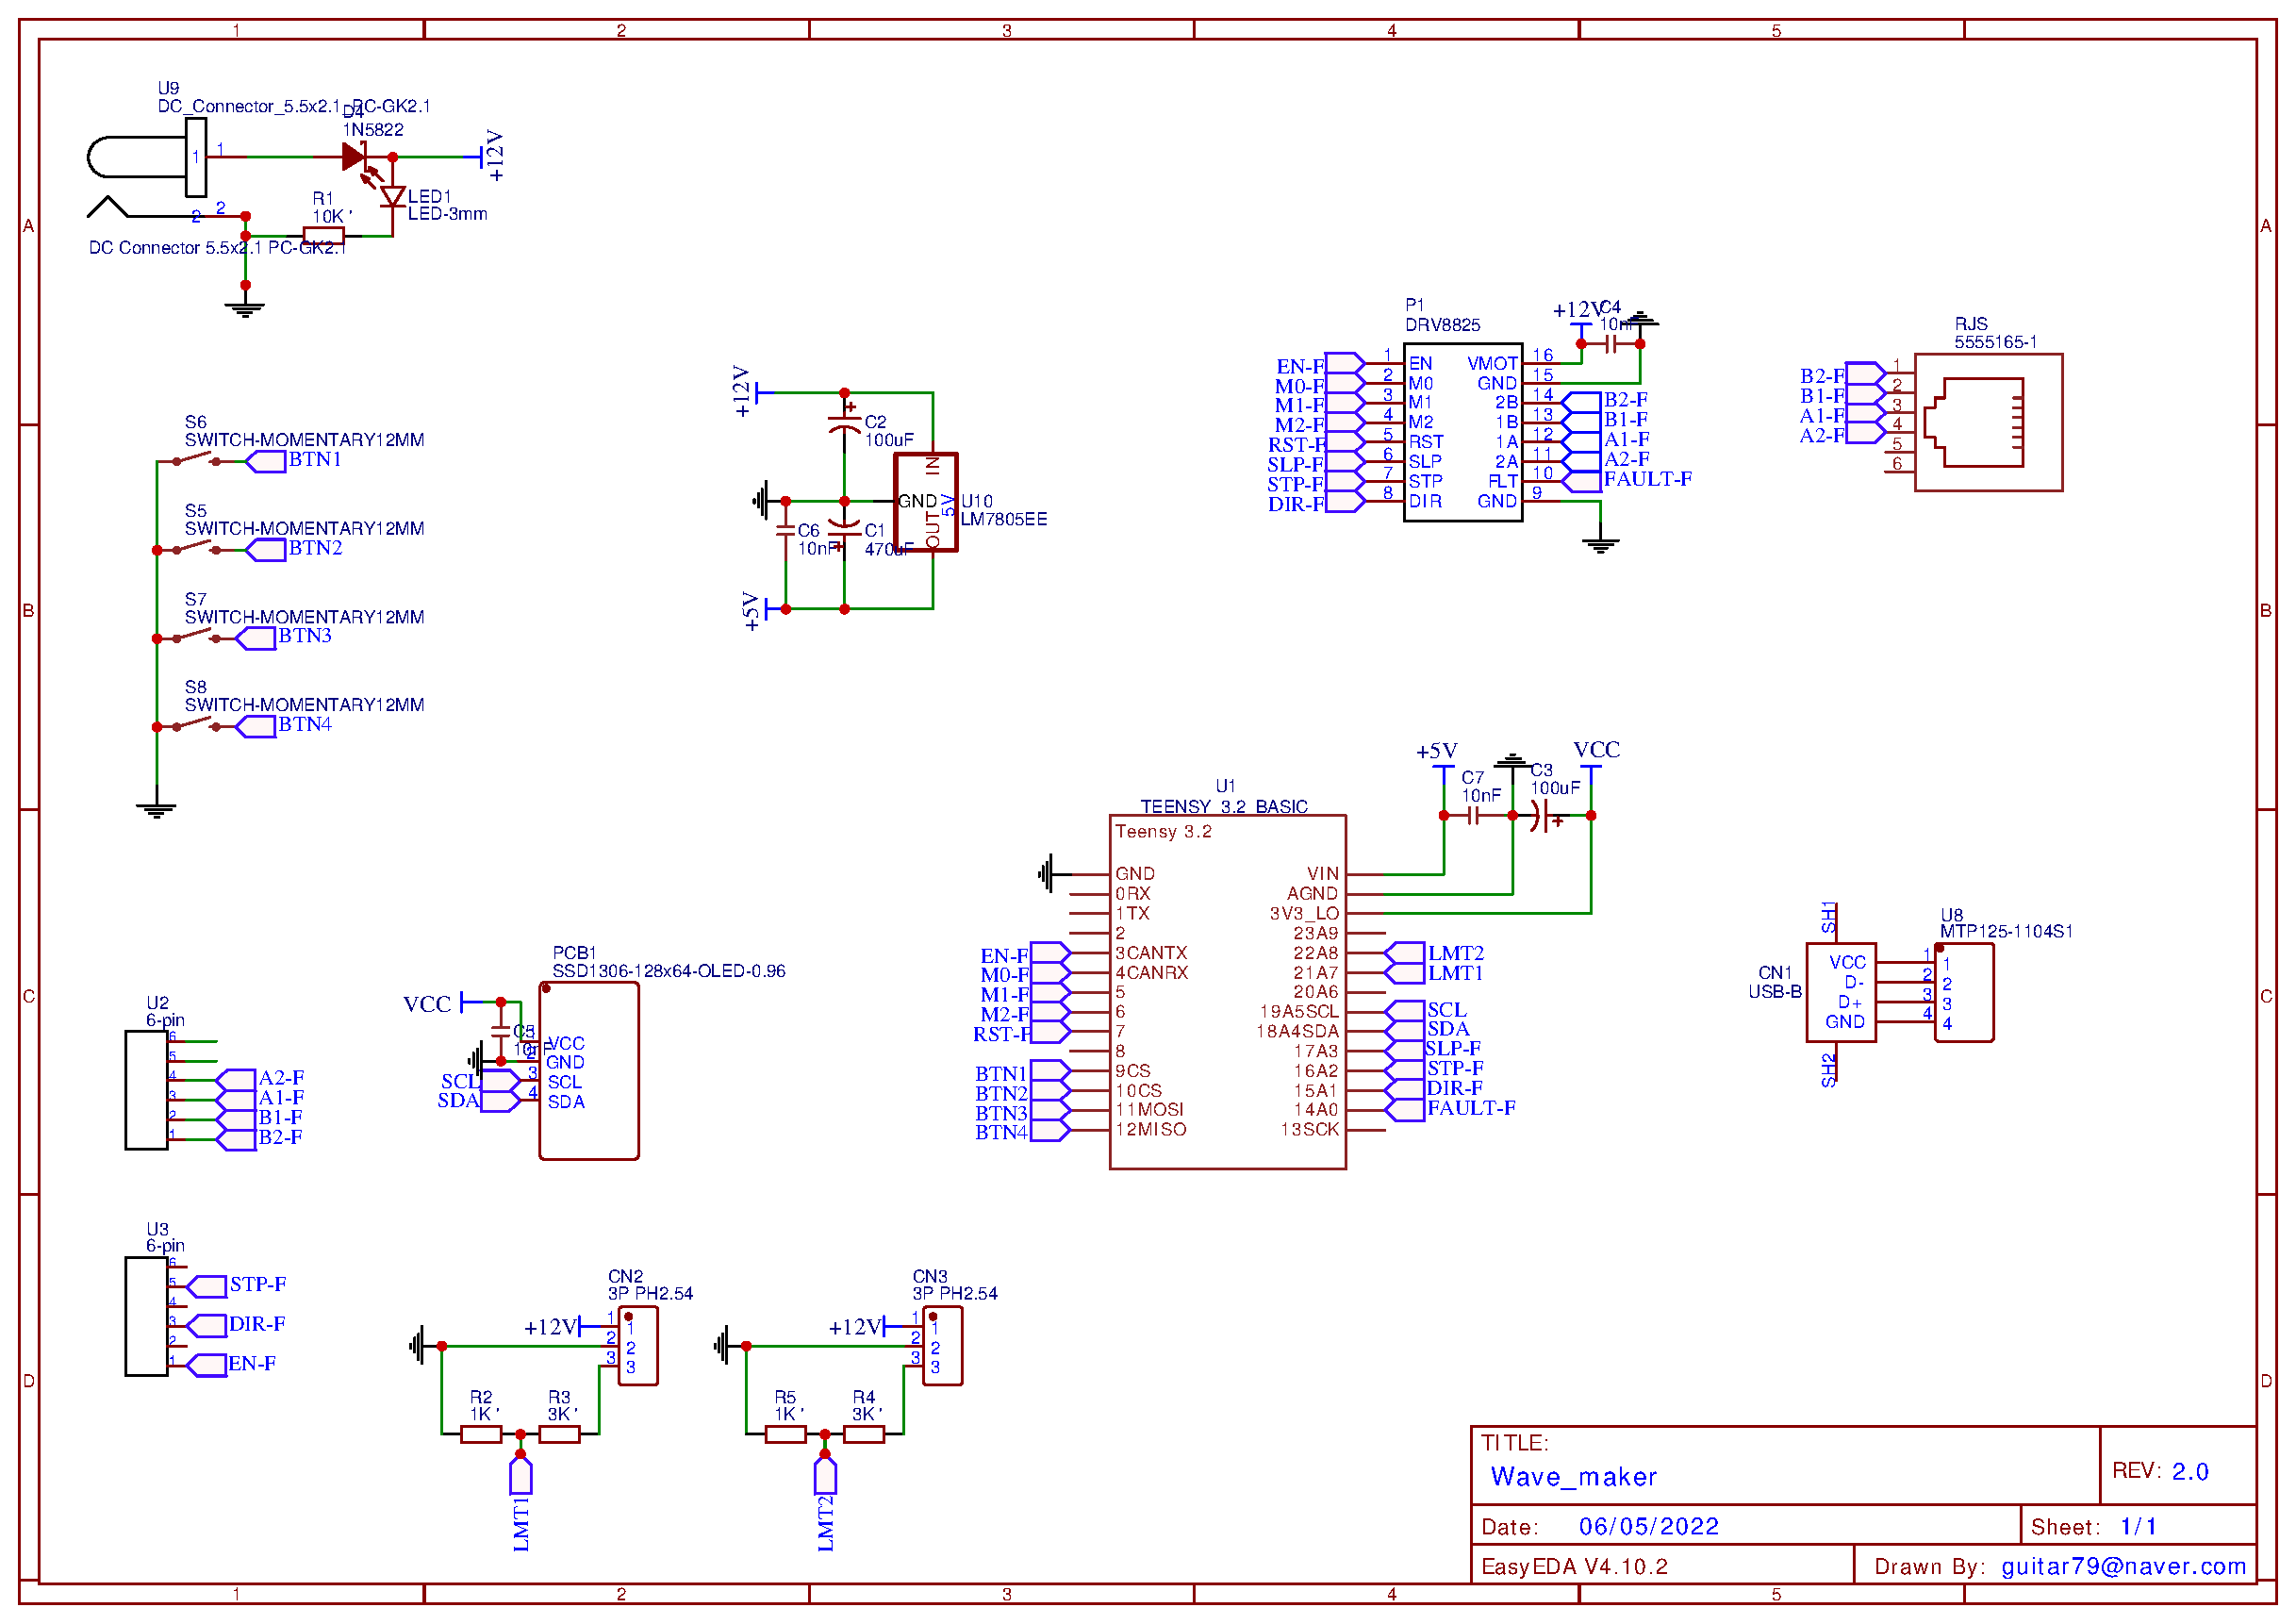
\includegraphics[height=5cm]{Schematic_Wave_maker_2-1_2022-11-24.pdf}
		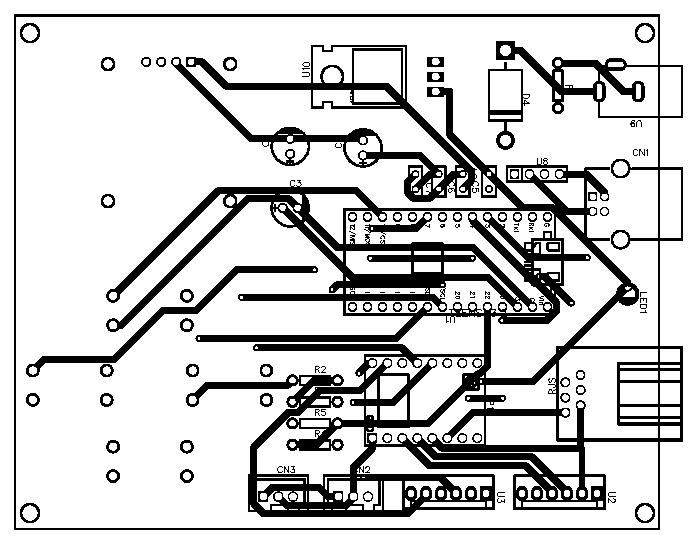
\includegraphics[height=5cm]{PCB_Wave_maker_2022-11-24.pdf}
        \caption{조파기 전자 회로 설계와 제작한 pcb}
		\label{PCB}
	\end{center}
\end{figure}


각 소자를 편리하게 다루기 위하여 pcb를 설계하였다. 틴지 보드 3.2는 $3.2~\mathrm{V}$의 구동 전압이 필요하며 상세 스펙은 다음과 같다(표 \ref{Specification of Teensy Board}).

\begin{table}[H]
    \centering
    \caption{조파기 전자 회로에 사용된 부품}
    \label{Specification of Teensy Board}
\begin{tabular}{l|llll}
\hline
ID & Name                             & \multicolumn{2}{l}{Designator}  & Quantity \\ \hline
1  & 10nF                             & \multicolumn{2}{l}{C6,C4,C7,C5} & 4        \\
2  & 470uF                            & \multicolumn{2}{l}{C1}          & 1        \\
3  & 100uF                            & \multicolumn{2}{l}{C2,C3}       & 2        \\
4  & USB-B                            & \multicolumn{2}{l}{CN1}         & 1        \\
5  & 1N5822                           & \multicolumn{2}{l}{D4}          & 1        \\
6  & LED-3mm                          & \multicolumn{2}{l}{LED1}        & 1        \\
7  & DRV8825                          & \multicolumn{2}{l}{P1}          & 1        \\
8  & 10KΩ                             & \multicolumn{2}{l}{R1}          & 1        \\
9  & 5555165-1                        & \multicolumn{2}{l}{RJS}         & 1        \\
10 & TEENSY\_3.2\_BASIC               & \multicolumn{2}{l}{U1}          & 1        \\
11 & 6-pin                            & \multicolumn{2}{l}{U2}          & 1        \\
12 & MTP125-1104S1                    & \multicolumn{2}{l}{U8}          & 1        \\
13 & DC\_Connector\_5.5x2.1\_PC-GK2.1 & \multicolumn{2}{l}{U9}          & 1        \\
14 & LM7805EE                         & \multicolumn{2}{l}{U10}         & 1        \\
15 & SSD1306-128x64-OLED-0.96         & \multicolumn{2}{l}{PCB1}        & 1        \\
16 & Momentary Switch                 & \multicolumn{2}{l}{S1,S2,S3,S4} & 4       
\\ \hline
\end{tabular}
\end{table}

ST-M5045는 리니어 액츄에이터의 모터를 조절하는 모터 드라이버이며 옆의 스위치의 조작에 따라서 스텝 수와 전류 값을 조절하여 외부적으로도 모터 회전의 감도를 바꿀 수 있다.

\begin{table}[H]
    \centering
    \captionsetup{justification=centering}
    \caption{ST-M5045의 스펙}
    \begin{tabular}{ll}
        \hline
        \textbf{DC power input type $(\mathrm{V})$}  & \textbf{24$\sim$50}      \\
        \textbf{Output current $(\mathrm{A})$}       & \textbf{1$\sim$4.5}      \\
        \textbf{Mircostep}           & \textbf{2, 4, 8, 16, 32, 64, 128, 256, 5, 10, 25, 50, 125, 250               }                \\
        Protect form        & Overheated, Short-voltage, over-voltage, over-current protection \\
        Maximum pulse rate $(\mathrm{kHz})$ & 300             \\
        Dimensions               & $120\mathrm{~mm} \times92\mathrm{~mm}\times33\mathrm{~mm}$ \\
        % Weight                   & \textless{}280g \\
        Working environment & Temperature~~-$15\sim40\mathrm{\degree C}$, Humidity~\textless{}$90\%$ \\ 
        \hline
    \end{tabular}
    \label{Specification of ST-M5045}
\end{table}

여러 소자를 연결하여 구성한 조파기의 제어부는 그림 \ref{Wavemaker}\와 같다.

\begin{figure}[H]
	\begin{center}
		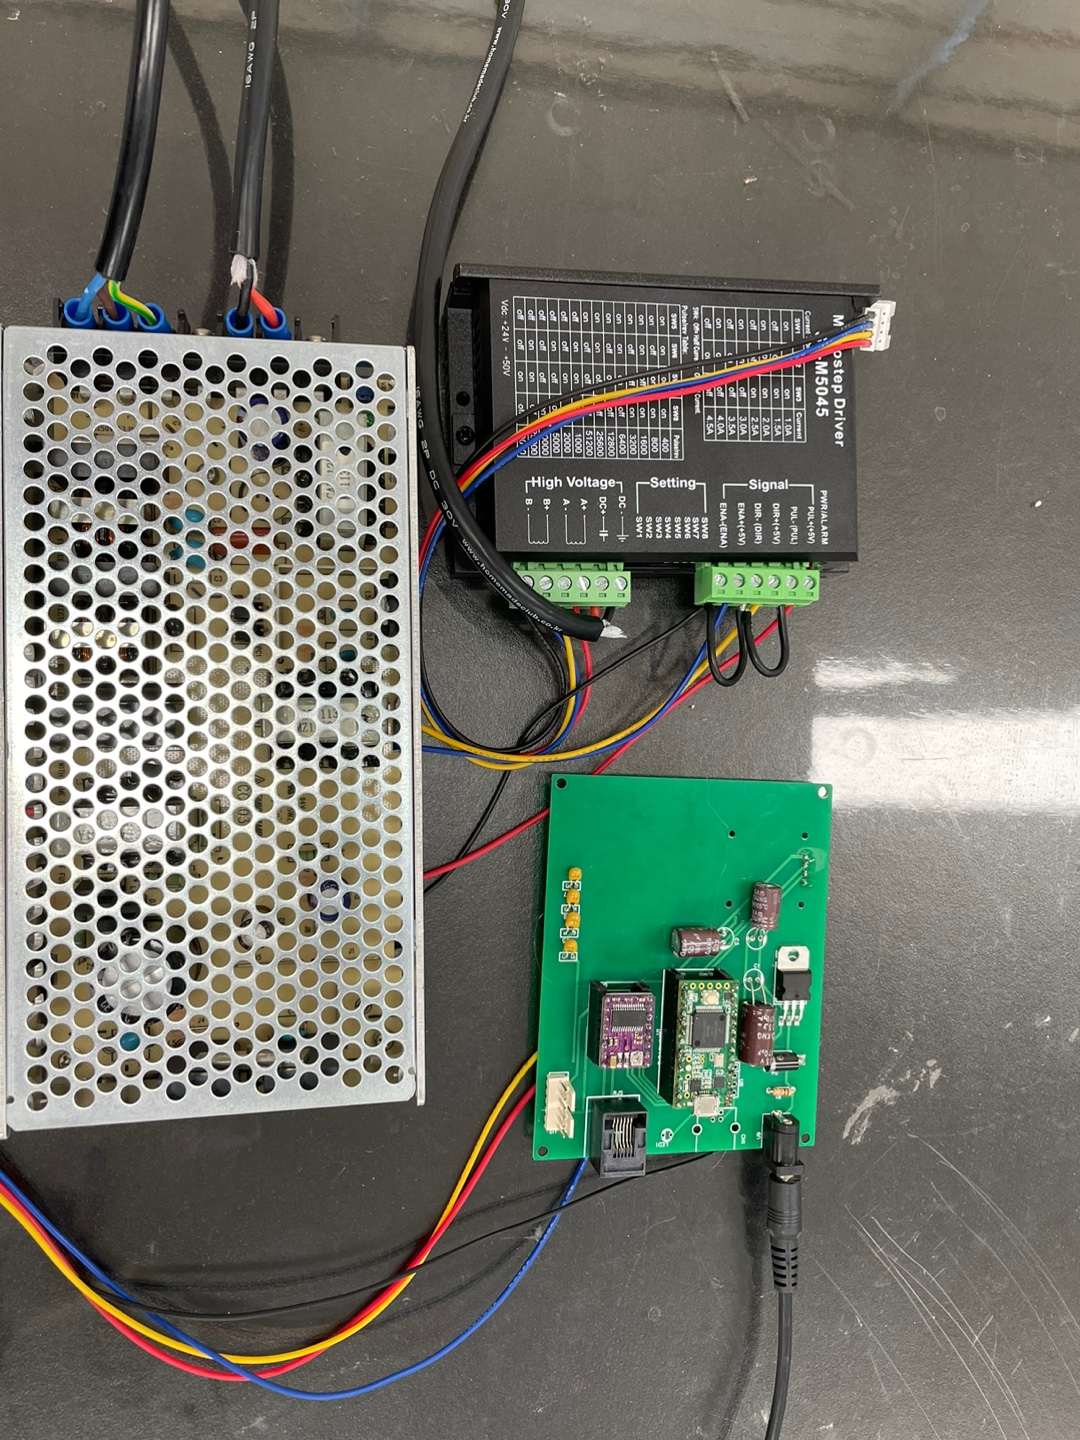
\includegraphics[clip, trim=0 100 100 100, angle=90, origin=c, width=.7\textwidth]{gdb}
		\caption{조파기 전자 회로와 모터 드라이버, 전원장치를 연결한 모습}
		\label{Wavemaker}
	\end{center}
\end{figure}

%Teensy Board 3.2, ST-M5045 스펙을 집어넣을 것.
%핀 연결은 Schematic이 있으니 굳이 따로 쓰지 말도록 하자.

% 하지만 파의 운동을 분석해보면 sin 파에 근접한 것이며 sin형으로 운동하도록 속도를 대입한 결과 판이 이상하게 운동하였다(그림 \ref{Motion of Motor}). 그리하여 제대로 sin형으로 운동할 수 있도록 다른 코드를 짰다. 조파기의 스텝 모터는 400 step 회전 시 $1~\rm{cm}$ 전진한다.

% \begin{figure}[H]
%     \centering
%     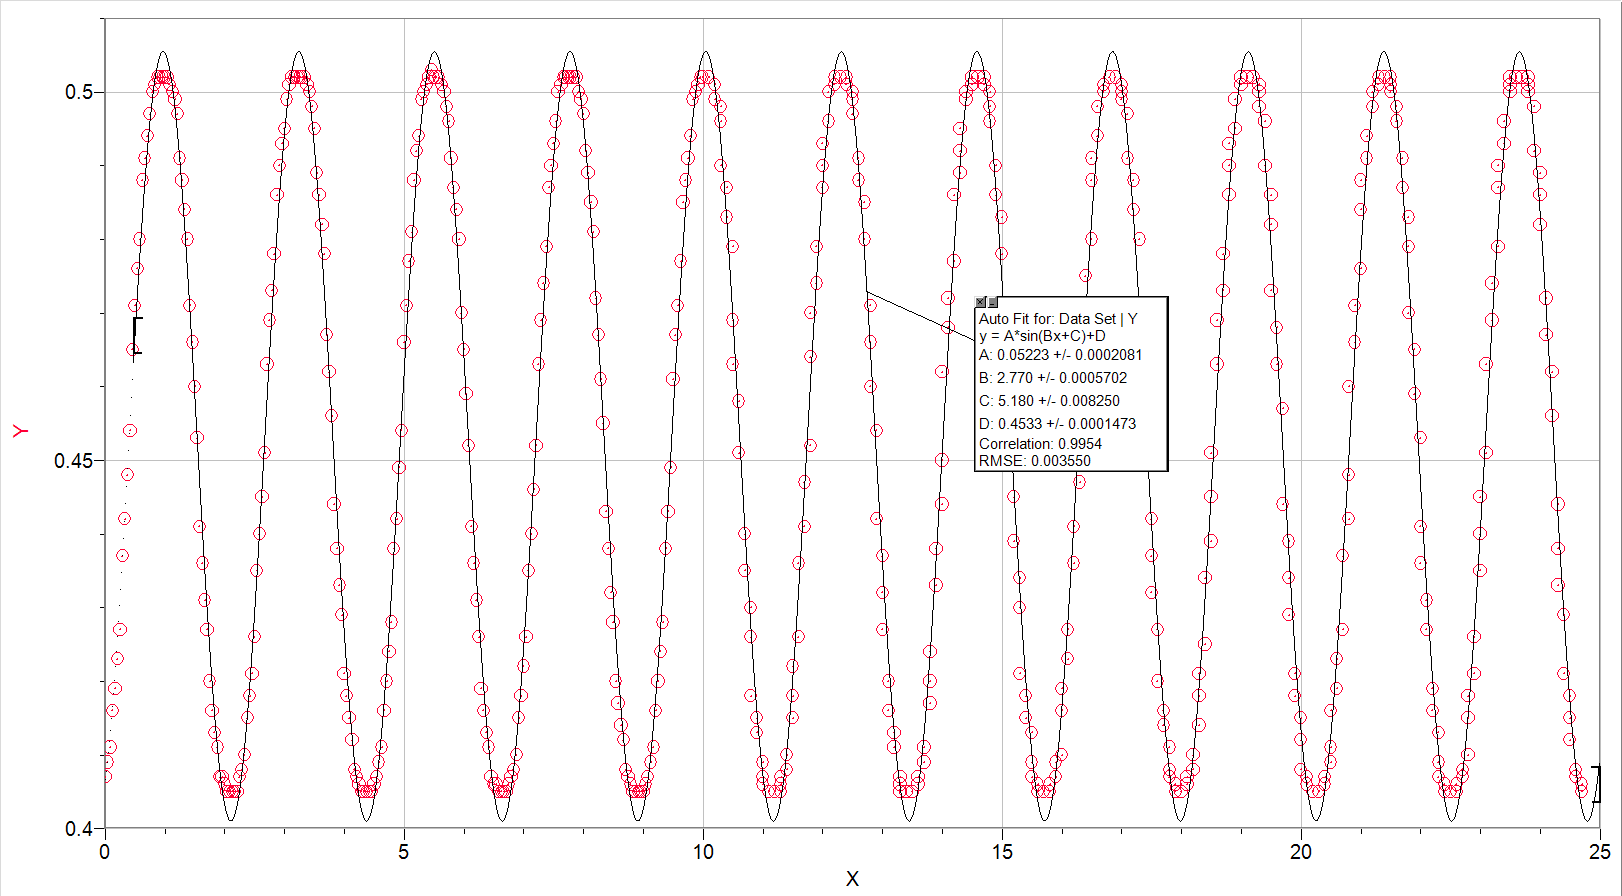
\includegraphics[height=4.5cm]{images/Linear_Motion.png}
%     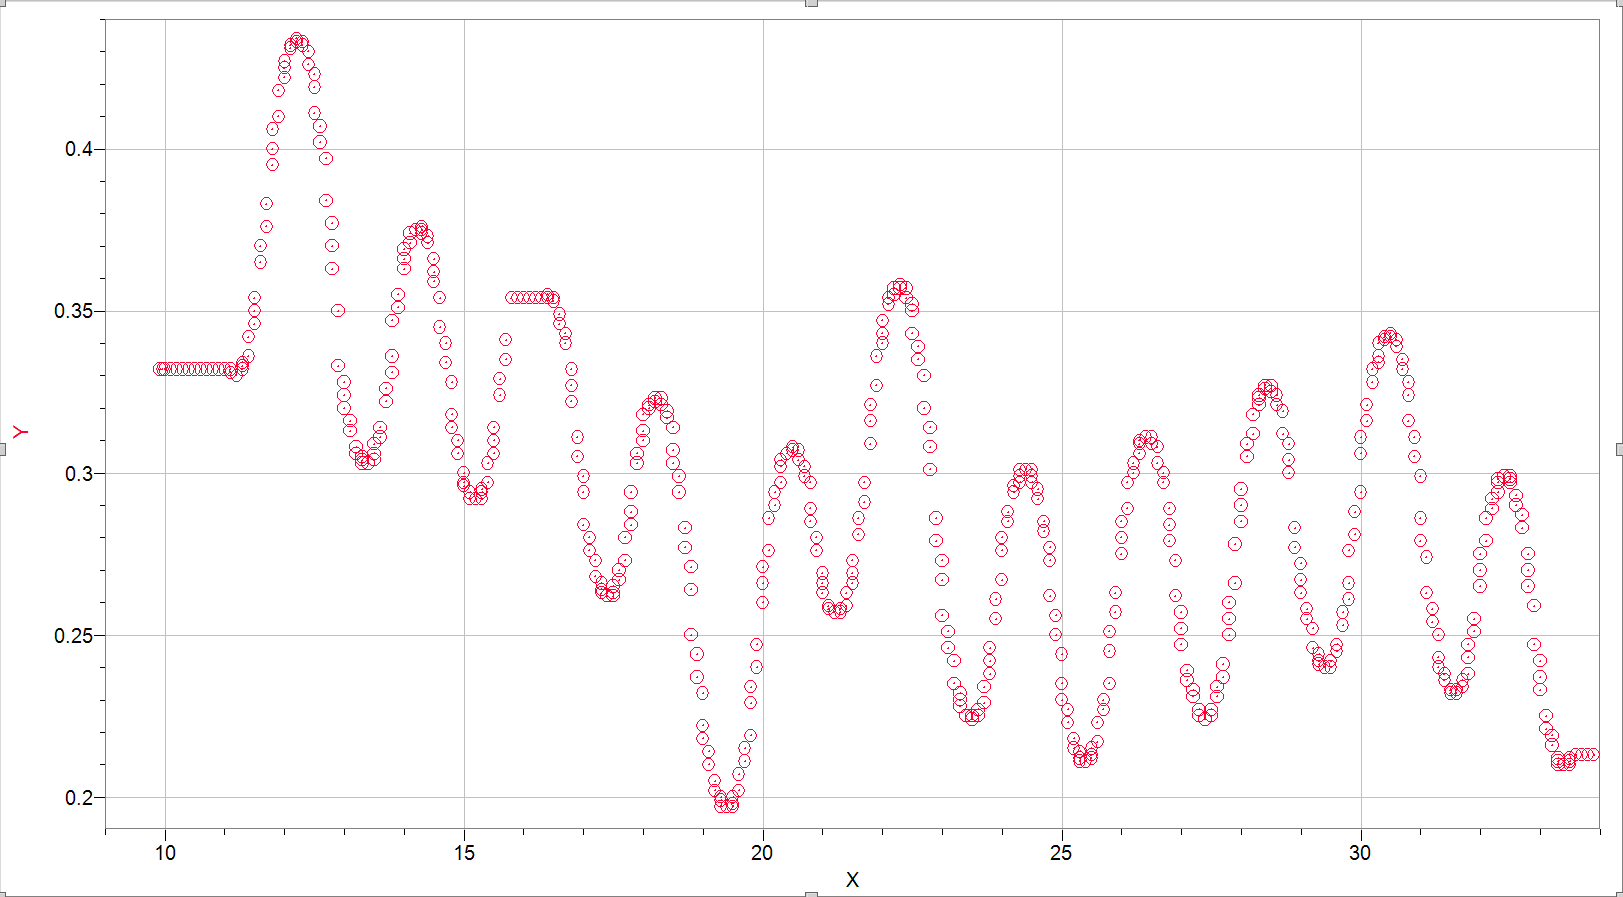
\includegraphics[height=4.5cm]{images/Sine_Motion.png}
%     \caption{모터의 선형 운동(좌)과 sin형 운동(우)}
%     \label{Motion of Motor}
% \end{figure}


\begin{figure}[H]
        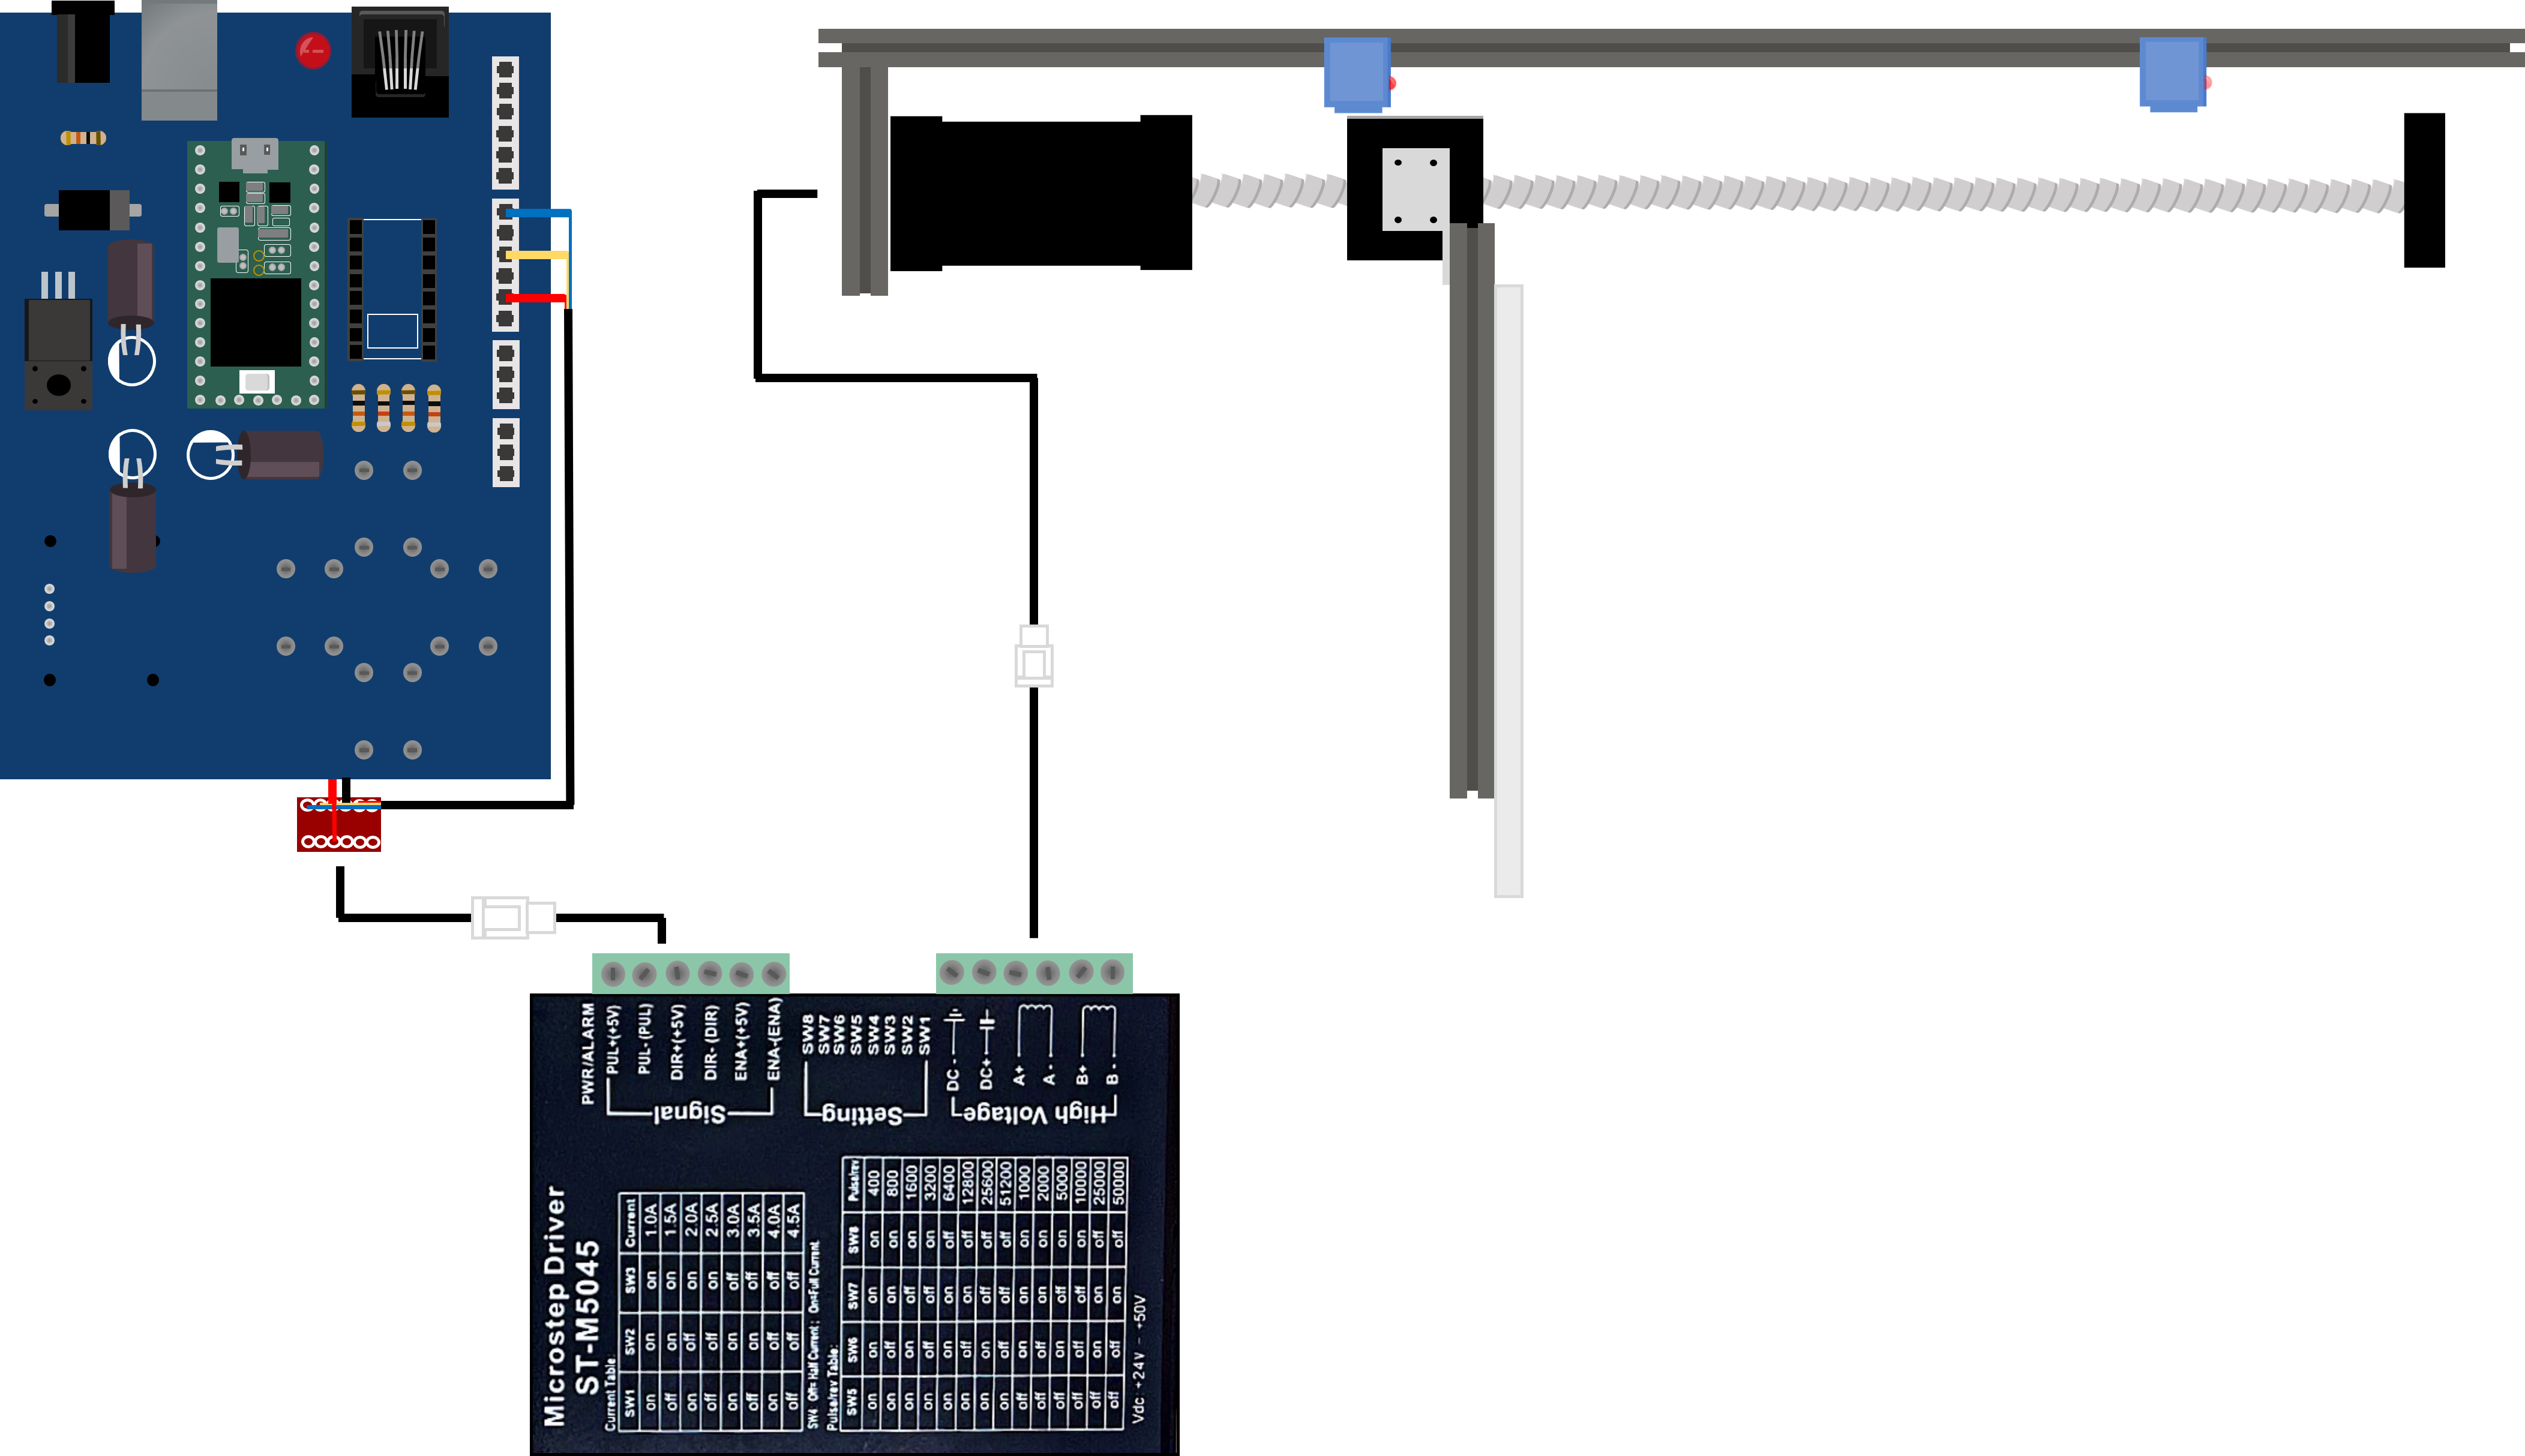
\includegraphics[width=0.9\textwidth]{images/wavemaker_control.png}
    \caption{조파기 전자 회로와 모터 드라이버, 전원장치를 연결한 모습}
    \label{wavemaker-structure}   
\end{figure}

%\subsubsection{소프트웨어}

코딩은 Arduino를 틴지 보드에 적용할 수 있도록 Teensyduino를 이용하였다. 스텝 모터 라이브러리는 AccelStepper, Stepper 등이 있으나 TeensyStep으로 모터를 더 빠르게 구동할 수 있다. 버튼과 연계하여 각 버튼을 누를 때마다 왼쪽, 오른쪽으로 특정 변위만큼 이동하도록 하였고 이를 반복하면 $\sin$에 근접한 파를 만들 수 있으나 근사적이며 직접 변위를 대입하는 방식으로 코드를 짜서 구동하였다.

\begin{figure}[H]
            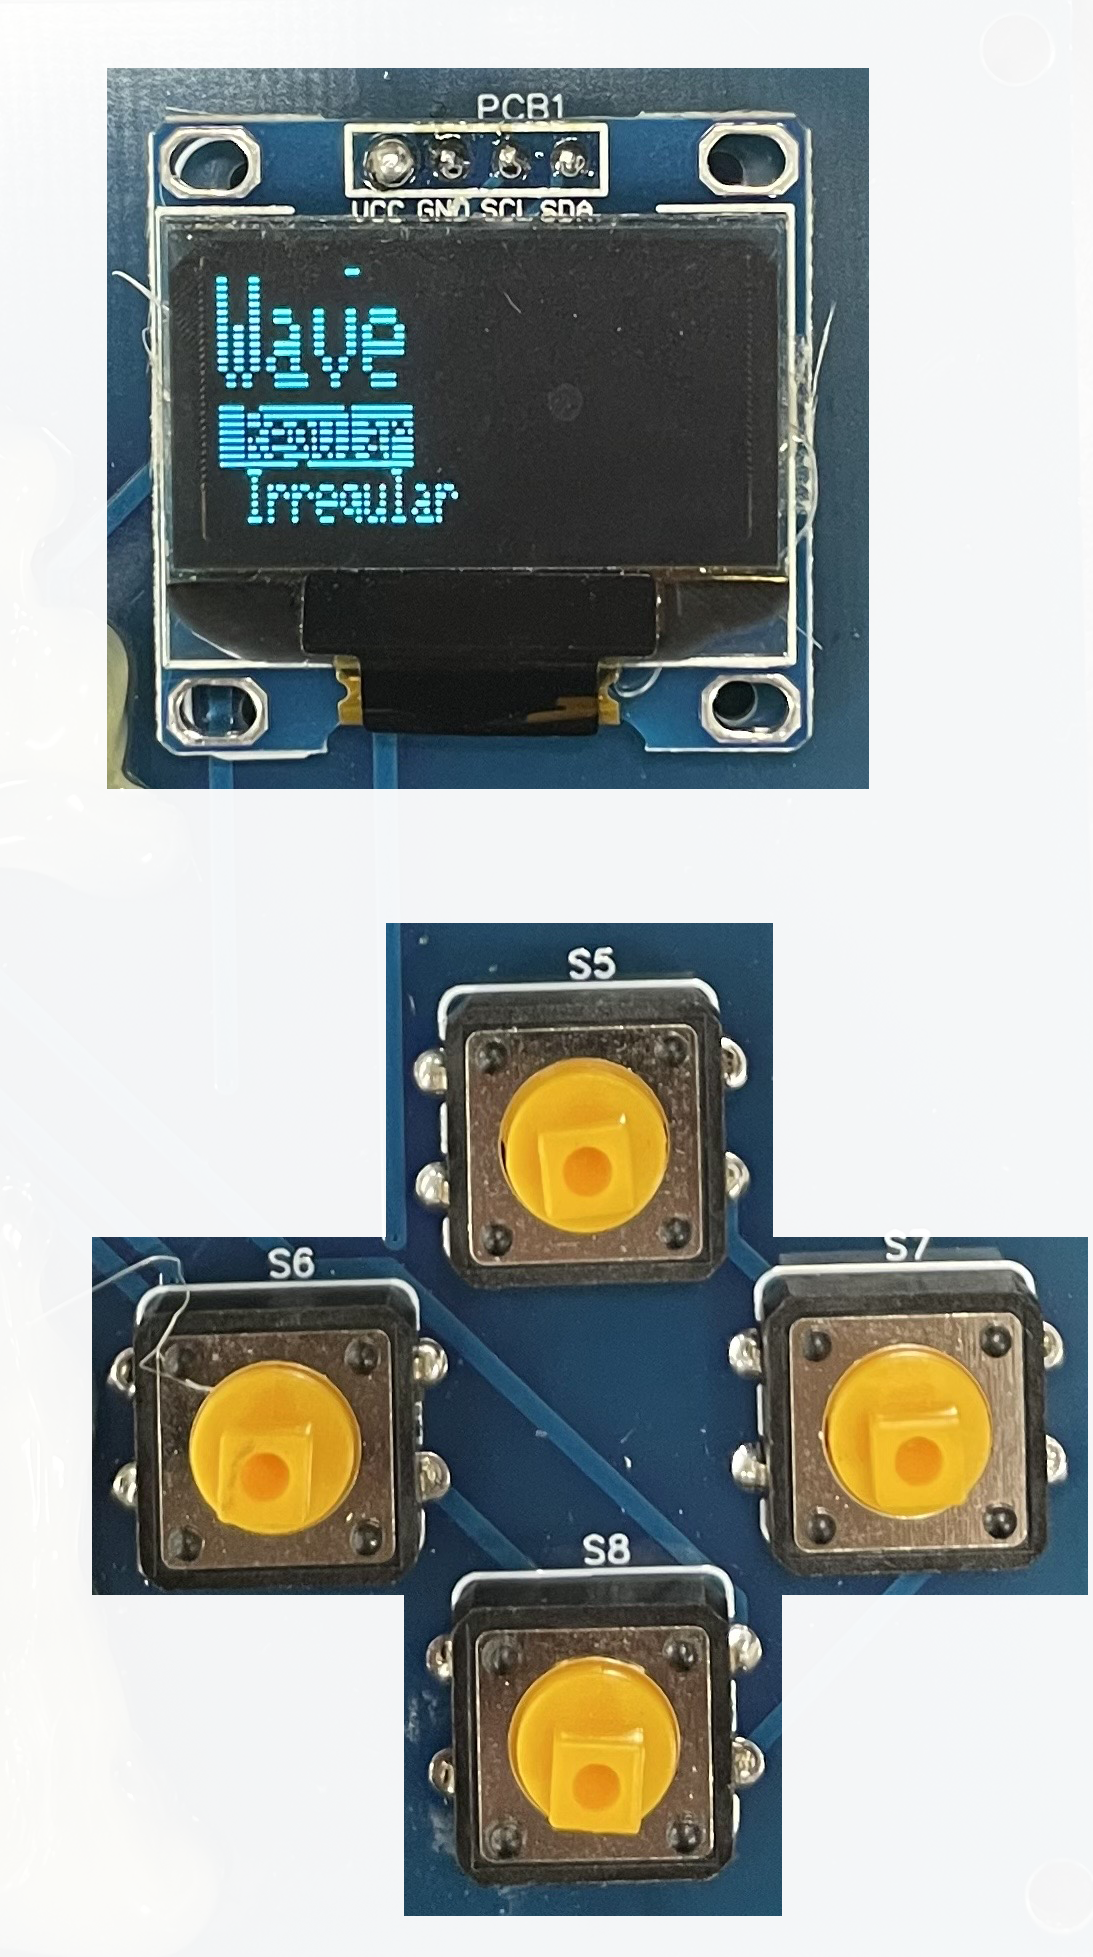
\includegraphics[trim=10 1050 100 0, clip, width=0.24\textwidth, height=3cm]{images/OLED1.png} 
            % (왼쪽, 아래(), 오른쪽, 위(숫자가 클수록 위에서 많이 잘림) )
            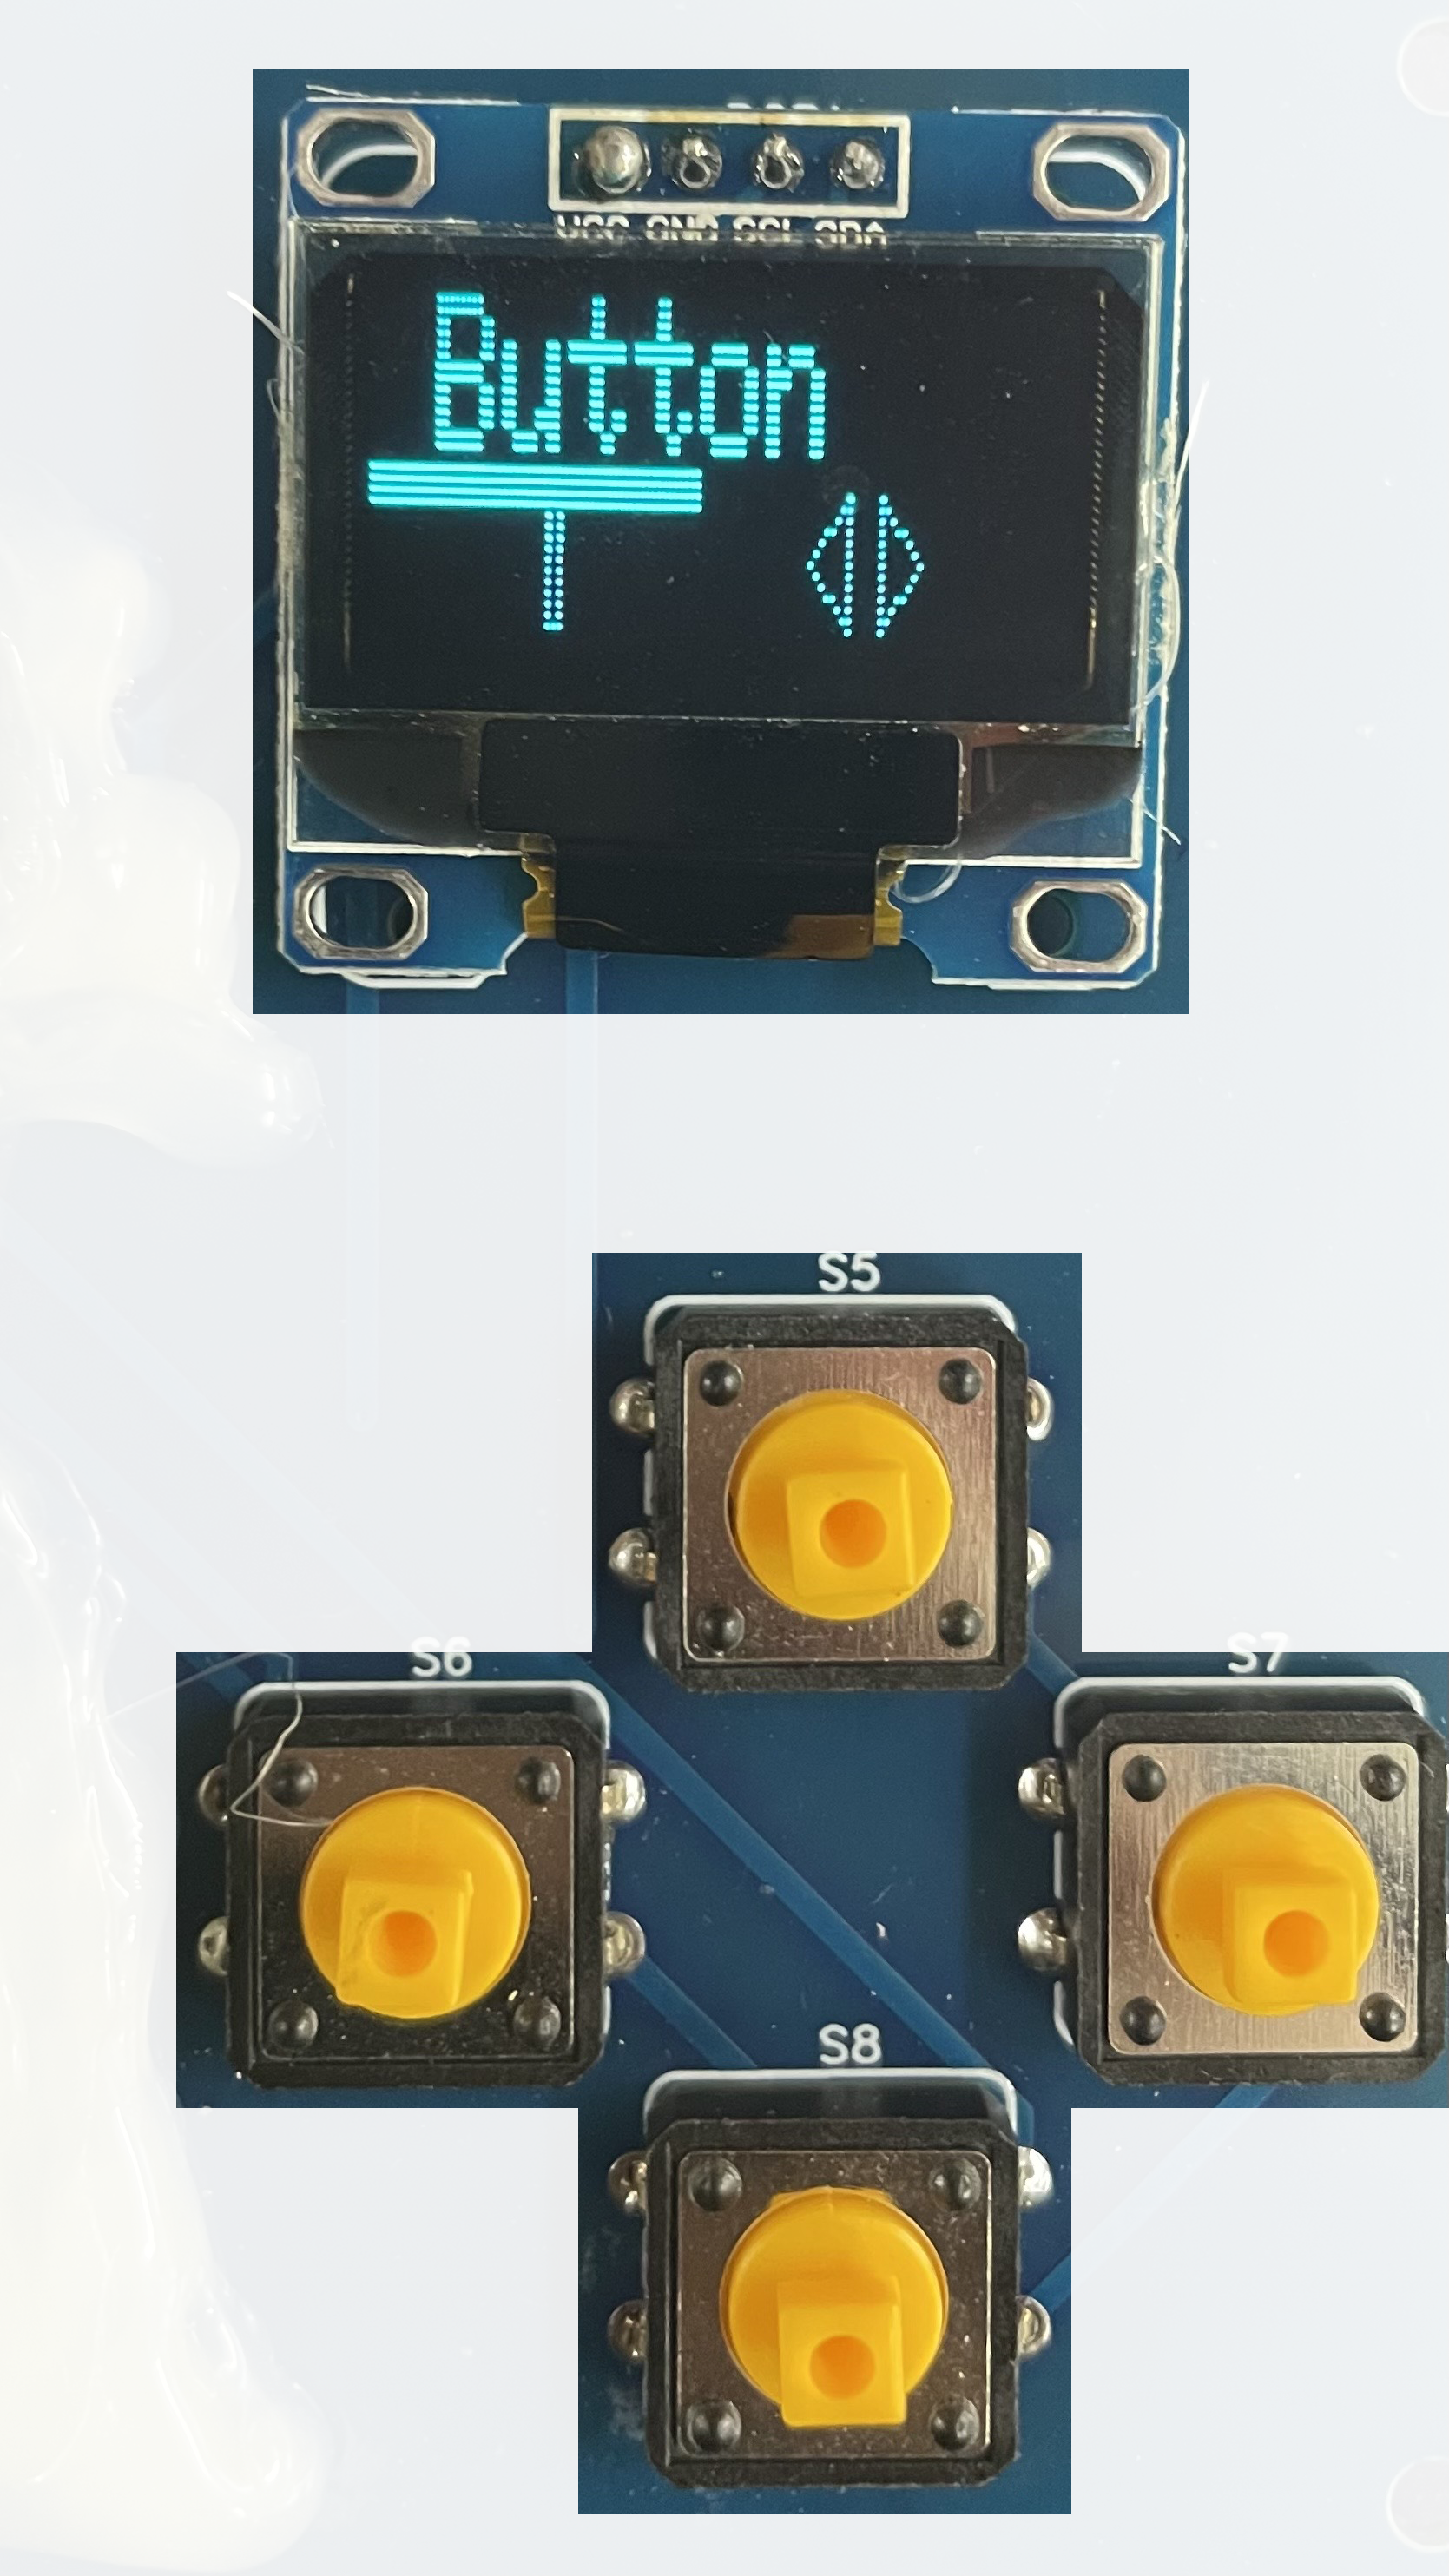
\includegraphics[trim=100 1550 100 0, clip, width=0.24\textwidth, height=3cm]{images/OLED2.png}
            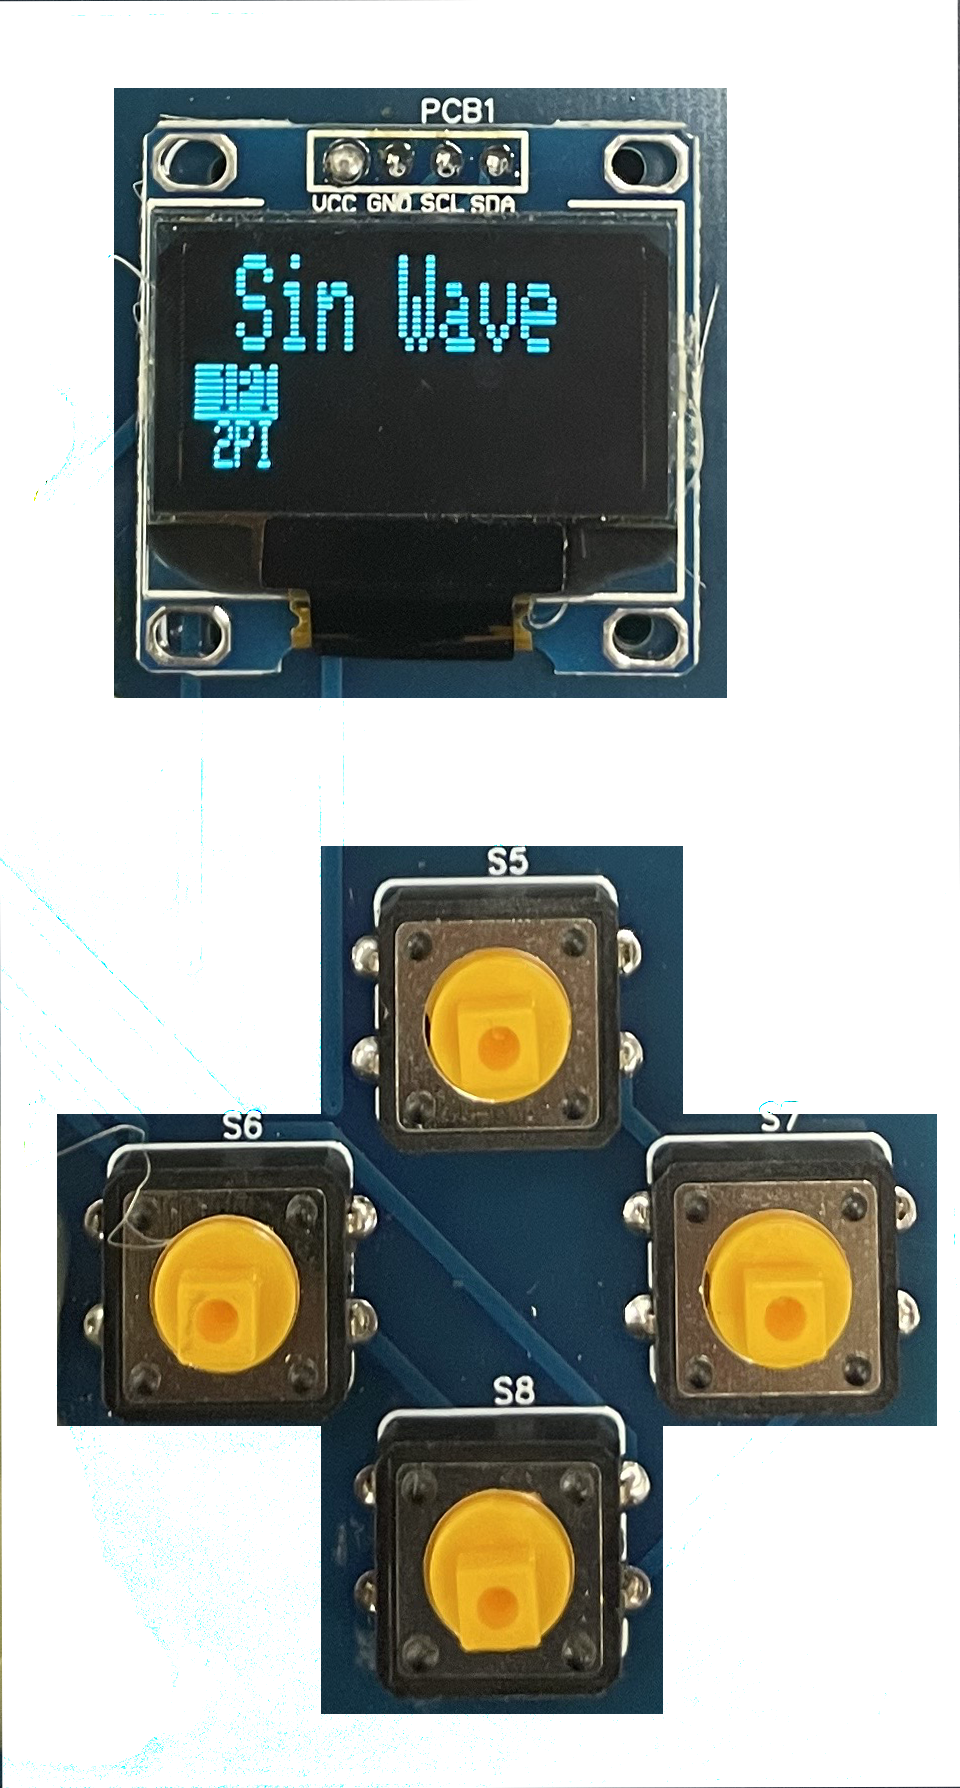
\includegraphics[trim=30 950 150 0,clip, width=0.24\textwidth, height=3cm]{images/OLED3.png}
            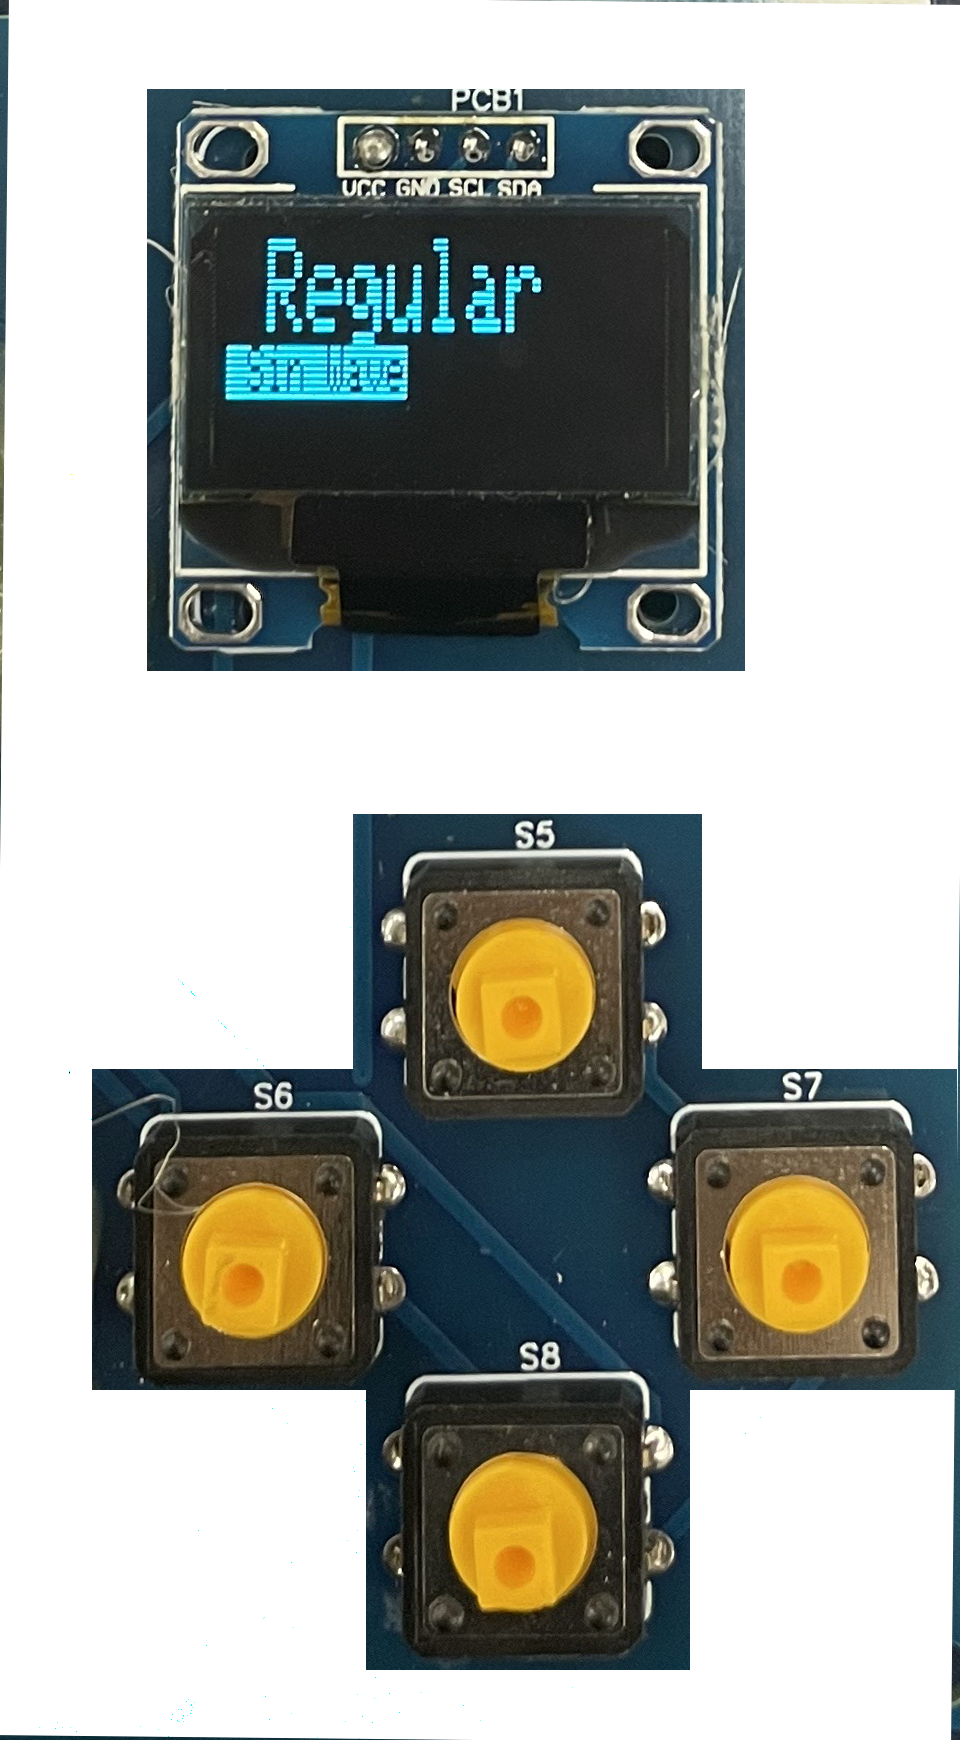
\includegraphics[trim=30 950 100 0, clip, width=0.24\textwidth, height=3cm]{images/OLED4.png}
        \caption{디스플레이 메뉴 동작 모습}
        \label{Oled}   
    \end{figure} 
    
전원을 켜면 Initialize가 실행된 후 메뉴 화면이 호출된다. 메뉴의 목록은 트리의 형태로 구성되어 있으며, Wave 항목 아래에 Regular Wave, Irregular Wave, Button이 있으며 버튼으로 각각의 하부 항목을 호출할 수 있다. Sin Wave의 항목에서는 변수 값 (액츄에이터의 진동 진폭, 진동수)을 선택해 원하는 값의 균형파를 생성할 수 있고, Button 항목에서는 원하는 방향으로 판을 움직일 수 있다.

\section{규칙파 검증 실험 및 결과}

\subsection{조파기 구동 코드}

\begin{algorithm}[h]
    \caption{Sinusoidal Motion}
    \label{Sinusoidal Motion}
    \begin{algorithmic}[1]
    \Procedure{Sinusoidal Motion}{$A, N, \Delta\phi$}\Comment{Move the motor by sinusoidal function}
        \For{$elapsed Time \geq 0$}
            \If{$elapsed Time \geq N$}
                \State {$elapsed Time$ = 0}
                \State {$target = f(n)$}%\Comment{In this case, $target$ = $A \sin${($n$ $\Delta$$\phi$)}}
                % \State {$target$ = $A \sin${($n$ $\Delta$$\phi$)}}
                \State {$n$ $\gets$ $n$ + 1}
                \State {Move $motor$ to $target$}
            \EndIf
        \EndFor
        \EndProcedure
    \end{algorithmic}
\end{algorithm}

조파기 구동 코드는 시간간격 $N~\mathrm{ms}$마다 각 변위를 $f(n)$으로 지정한다 (알고리즘 \ref{Sinusoidal Motion}). 함수가 $\sin$이면 모터가 $\sin$ 각 변위를 따라 움직일 것으로 기대할 수 있다. $\sin$형 구동을 위한 코드의 $f(n)$은 다음과 같다.
\begin{equation}
    f(n) = A \sin(n \Delta\phi)
    \label{f(n)}
\end{equation}

실질적인 매개변수는 $A, \omega, N$이며 $A$는 진폭, $\omega$는 조파판 위상의 각진동수, $N$은 조파판의 변위를 업데이트하는 시간 간격이다. $\omega$는 다음과 같이 정의될 수 있다.
\begin{equation}
    \omega = \frac{\Delta\phi}{\Delta t} = \frac{\Delta\phi}{N}, ~\Delta\phi = N \omega
    \label{f(N)}
\end{equation}

$N$과 $\omega$가 매개된 입력 신호의 식이 실질적인 매개변수 표현이며 $A$와 $\omega$는 코드에서의 입력값과 조파기 구동 시 판의 움직임에서 실제로 나타나는 값이 달라 그 관계를 파악하기 위한 실험이 필수적이고 $\omega$가 너무 큰 경우 탈조가 날 수 있어 가능 범위를 파악해야 한다. $N$은 이론적으로 조파판의 움직임에 영향을 주지 않아 고정하여 실험을 진행했으나 판의 최대 변위와 최소 변위 지점에서 변위가 업데이트되어야 하므로 각진동수에 따른 $N$의 변화가 필요할 수 있다.

\subsection{예비 실험}
$A = 5\mathrm{~cm}$, $N=50$의 고정된 값에서 $\omega$를 $0.4\pi$에서 $\pi$까지 $0.1\pi$ 간격으로 변화시키며 실험하고 추가로 $1.5\pi$에 대해서도 실험했다.
판의 움직임을 분석했을 때 $\omega$가 증가함에 따라 진폭의 출력값이 감소하다. 생성파는 $\sin$파와 유사하였고 각진동수는 입력값과 동일했지만 진폭은 관계가 없어 실험 구성 단계에서는 모터의 움직임만 분석하였다.

\subsection{실험 구성}
생성파의 분석이 필요치 않으므로 조파기의 모터 대신 작은 모터에 회로를 연결하여 모터의 움직임이 $\sin$ 형태인지 확인하였다. 시리얼 모니터에 각 위치를 출력하여 알 수 있으며 출력값은 입력값과 일치하나 진폭은 달랐으며, $\omega$가 클수록 진폭의 출력값이 감소하였다. 즉, 파를 생성할 때 구동 코드의 매개변수에 따른 판의 움직임과 생성되는 파 2개를 관찰해야 하고 두 파의 진폭과 각진동수를 코드의 값과 비교하여 관계를 파악하는 것을 목표로 한다.

\begin{figure}[H]
    \centering
    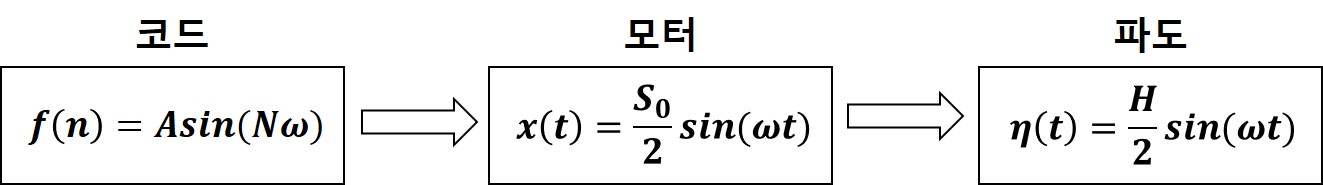
\includegraphics[width=12cm]{images/Flow_Chart(Analysis System_Kor).jpg}
    \caption{조파기 검증 실험의 흐름도}
    \label{Flow_Chart}
\end{figure}

$S_0$와 $A$의 직접적인 관계는 알 수 없으나 $S_0$와 $H$의 관계는 이론적 배경의 식을 따를 것으로 기대할 수 있으며 파가 $\sin$형이 아니더라도 FFT 분석을 통해서 $\omega$를 구할 수 있고 세 파동에서 일관될 것이다. 제대로 검증하기 위해서는 다양한 조건에 대한 데이터가 필요하며 이론적 분석과 예비 실험을 통해 정한 범위는 $A$는 $1\mathrm{~cm}$부터 $10\mathrm{~cm}$까지 $1\mathrm{~cm}$ 간격으로, $\omega$는 $3$부터 $12$까지 $1$ 간격으로 변화시키는 것이다. $N$은 50으로 고정시켰다 (단, 수심은 $15\mathrm{cm}$로 고정하였다).

%실험한 내용을 집어넣어야 함.

%실험계의 모식도가 필요함. 혹은 사진이라도.

조파기로 여러 형태의 파도를 생성하며 실험을 진행하였다. 그림 \ref{result-wave}\는 조파기로 파도를 만드는 모습과 생성된 해파가 전파되는 모습을 동영상으로 촬영한 후 캡쳐하여 나타낸 것이다. 

\begin{figure}[hbp]
    \centering
            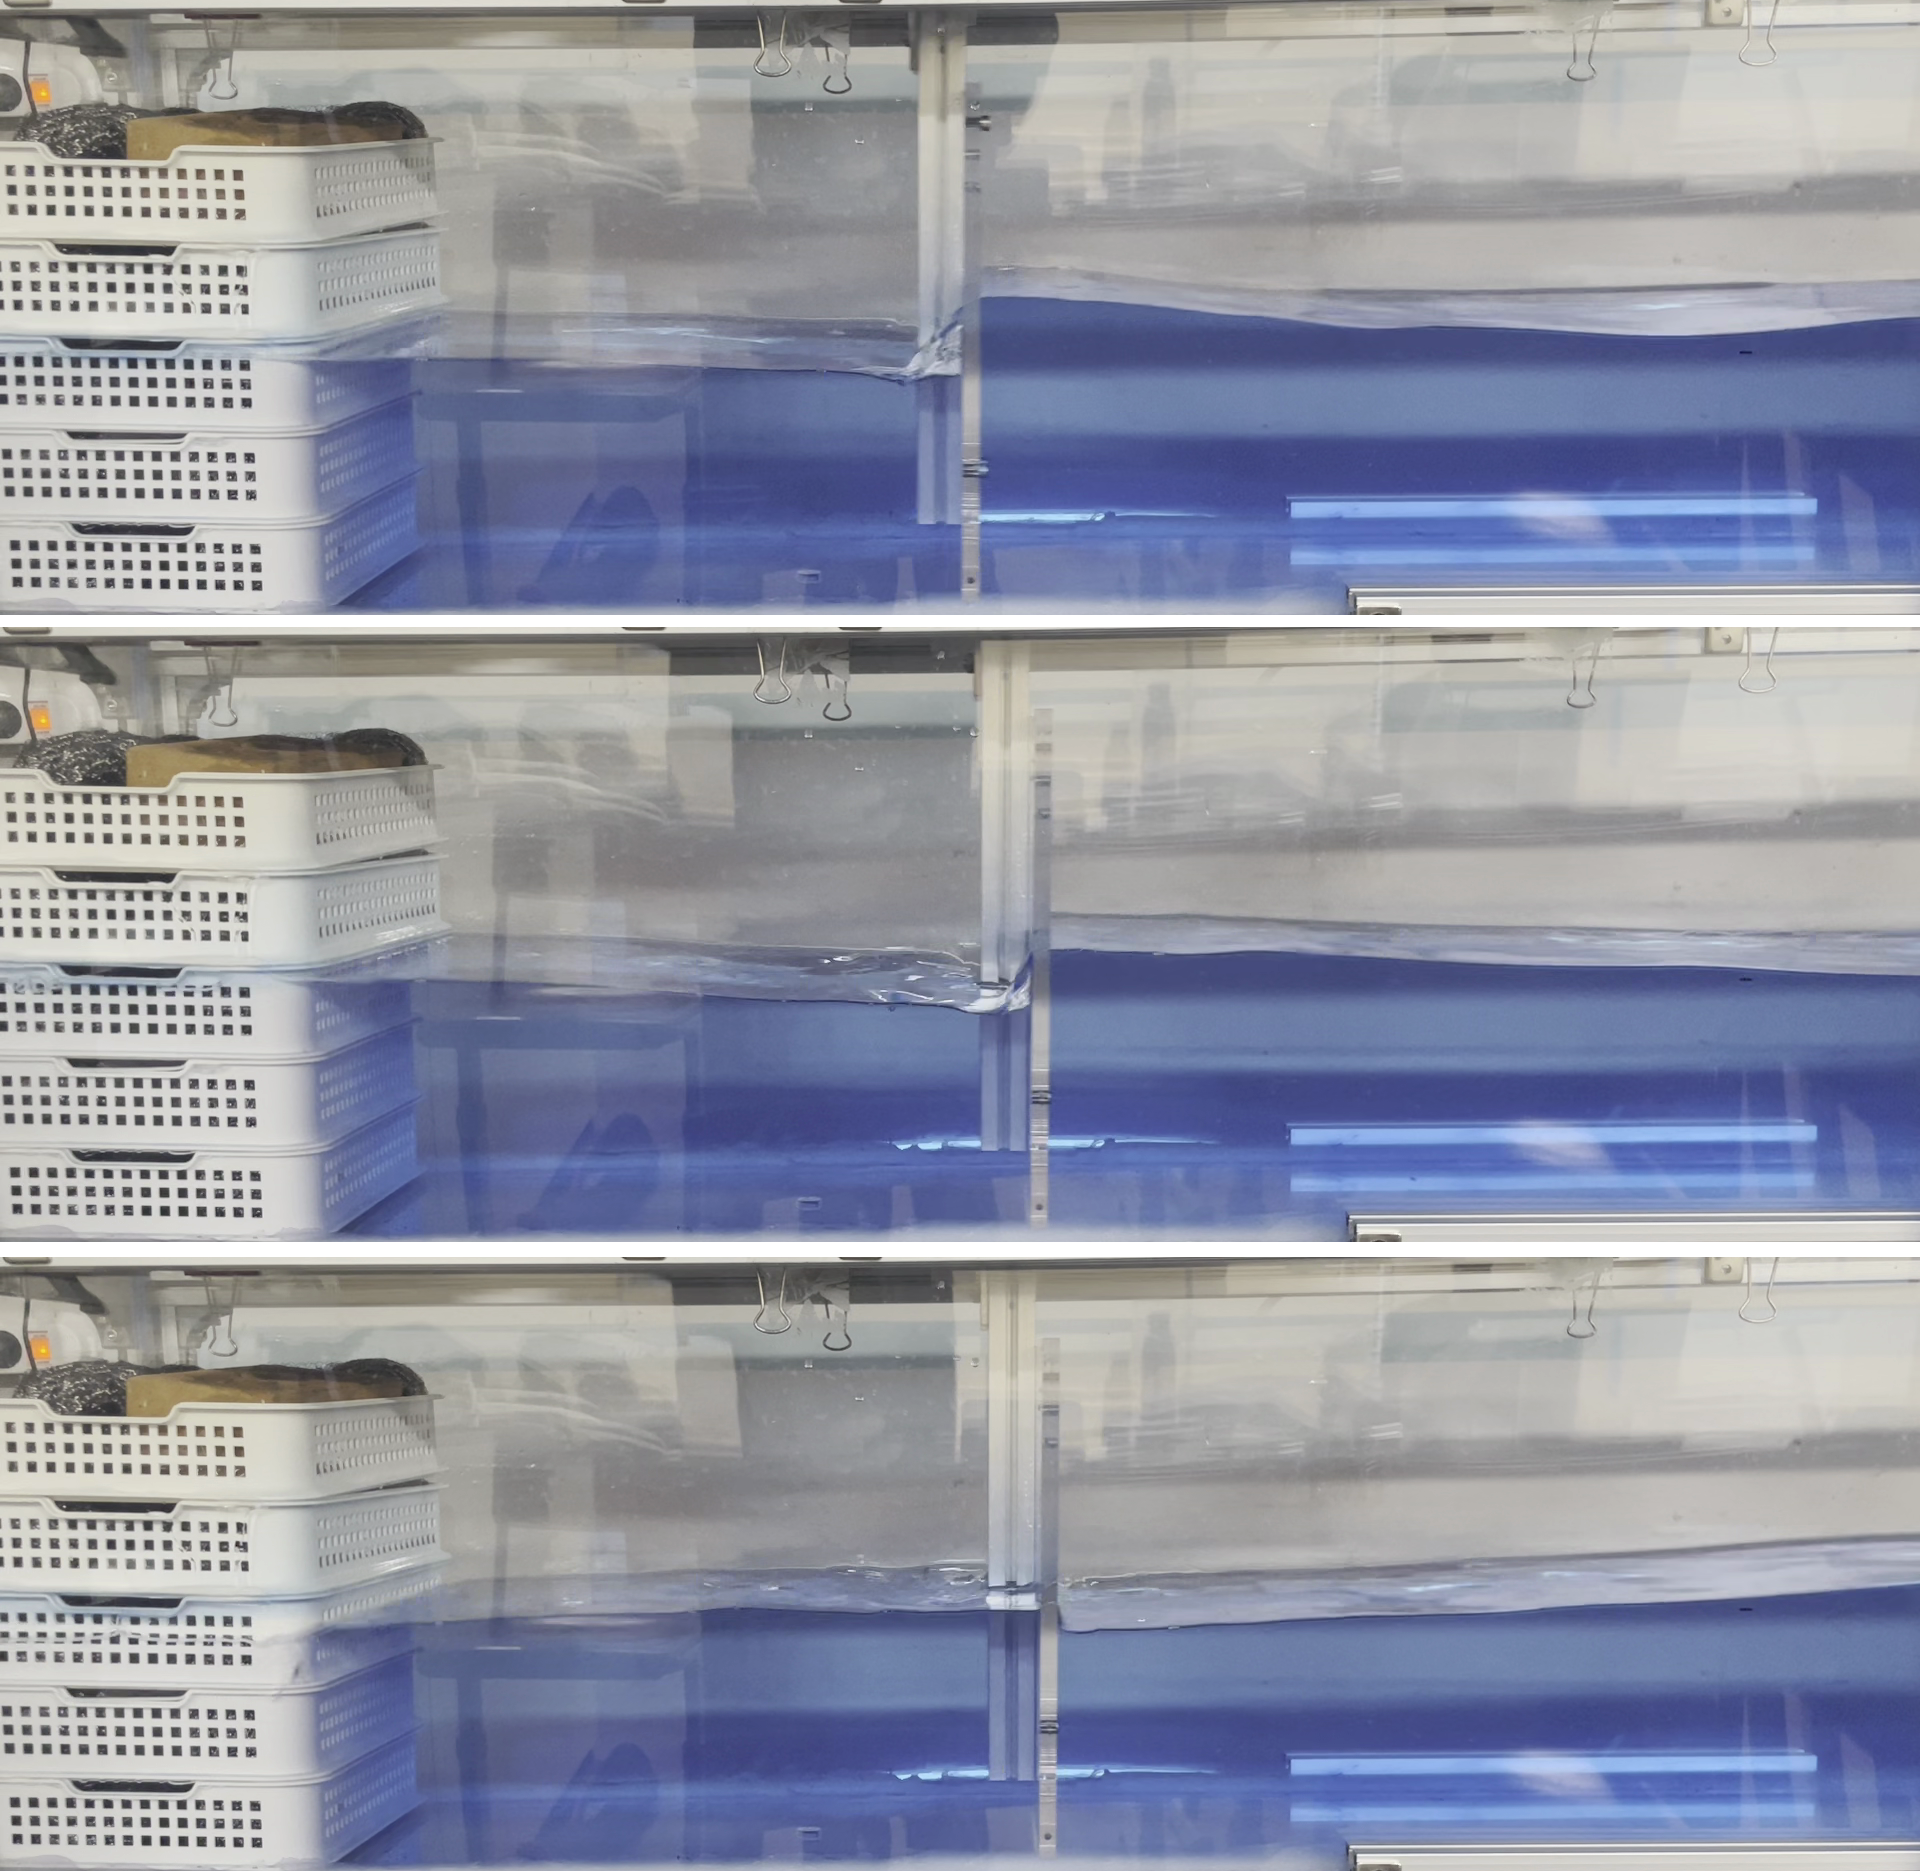
\includegraphics[trim=0 0 0 0, clip, width=0.45\textwidth, 
                height=8cm,
                ]
                {images/vlcsnap-2023-06-29-10h35m08s932-1.png} 
            % (왼쪽, 아래(), 오른쪽, 위(숫자가 클수록 위에서 많이 잘림) )
            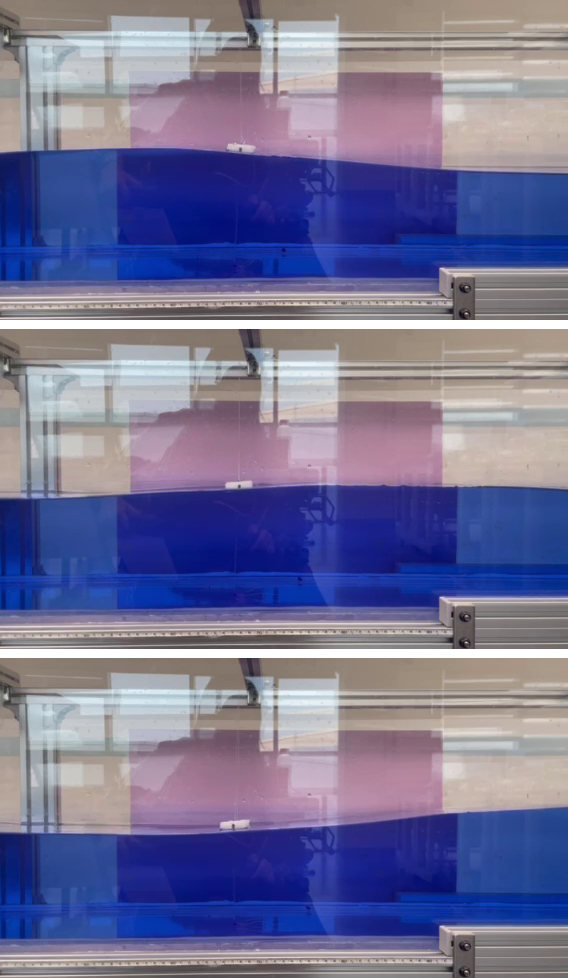
\includegraphics[trim=0 0 0 0, clip, width=0.45\textwidth, 
                height=8cm,
                ]
                {images/vlcsnap-2023-06-29-10h53m08s226-1.png} 
        \caption{(a) 조파기로 파도를 만드는 동작 (b) 생성된 파도가 전파될때 파고를 측정하는 모습}
        \label{result-wave}   
        \begin{tikzpicture} [remember picture, overlay, anchor=north west, inner sep=0pt]
            \node [%draw=yellow, 
                    text=yellow,
                    ] at (-8, 9) {(a)};
            \node [%draw=yellow, 
                    text=yellow,
                    ] at (0.1, 9) {(b)};
         \end{tikzpicture}	 
\end{figure}    

\subsection{성능 검증 실험 결과}

% \begin{figure}[H]
%     \centering
%     \begin{tabular}{ll}
%         \begin{filecontents*}{A.dat}
% w_msr	A_thm	A_msr
% 0.6272	10	9.515
% 0.6275	10	9.532
% 0.6541	10	9.523
% 0.6681	10	9.499
% 0.6826	10	9.48
% 0.6978	10	9.456
% 0.6978	10	9.449
% 0.7849	10	9.326
% 0.785	10	9.318
% 0.8263	10	9.26
% 0.8971	10	9.138
% 0.8971	10	9.137
% 1.047	10	8.883
% 1.047	10	8.876
% 1.256	10	8.498
% 1.256	10	8.492
% 1.57	10	7.916
% 1.57	10	7.903
% 1.744	10	7.588
% 1.962	10	7.206
% 1.962	10	7.197
% 2.093	10	6.988
% 2.093	10	6.978
% 2.243	10	6.749
% 2.415	10	6.489
% 2.617	10	6.218
% 2.618   10	6.214
% 3.141	10	4.837
% 3.141	10	4.837
% 3.927	10	3.093
% 5.236	10	0.5795
%         \end{filecontents*}

%         \begin{tikzpicture}[
%                 %Environment Cfg.
%                 %font=\bfseries\sffamily,
%             ]
%             \begin{axis}[
%                 width=6cm,
%                 height=6cm,
%                 at={(0,0)},
%                 ymin=0,
%                 ymax=13,
%                 xmin=0,
%                 xmax=6,
%                 grid=both,
%                 minor tick num =5,
%                 minor tick style={draw=none},
%                 minor grid style={thin,color=black!10},
%                 major grid style={thin,color=black!10},
%                 %ylabel style={rotate=90},
%                 ylabel={$A_{plate}~\left[\mathrm{~cm}\right]$},
%                 xlabel={$\omega_{msr}~\left[\mathrm{~rad/s}\right]$},
%                 tick align=outside,
%                 axis x line*=middle,
%                 axis y line*=none,
%                 xtick={0,2,...,16},
%                 ytick={0,2,...,16},
%                 %xlabel style={color=blue!50!cyan},
%                 %ylabel style={align=center,rotate=-90,color=blue!50!cyan},
%                 x tick label style={
%                     /pgf/number format/assume math mode, font=\sf\scriptsize},
%                 y tick label style={
%                     /pgf/number format/assume math mode, font=\sf\scriptsize},
%                 legend cell align = {left},
%                 legend pos = north west,
%                 legend style={nodes={scale=0.5, transform shape}},
%                 ]
%                 \addplot [%only marks, 
%                     mark size=1pt,
%                     mark=o, 
%                     %mark options={solid}, 
%                     %smooth,
%                     ] 
%                 table [x=w_msr, y=A_thm] {A.dat};
%                 \addlegendentry{$A_{thm} - \omega_{msr}$}
%                 \addplot [%only marks, 
%                     mark = +,
%                     mark size=1pt,
%                     ]
%                 table [x=w_msr, y=A_msr] {A.dat};
%                 \addlegendentry{$A_{msr} - \omega_{msr}$}
%             \end{axis}
%         \end{tikzpicture}
        
%         &
        
%         \begin{filecontents}{B.dat}
%                     wthm   wPlate
% 0.6283	0.6272
% 0.6981	0.6978
% 0.7854	0.785
% 0.8976	0.8971
% 1.0472	1.047
% 1.2566	1.256
% 1.5708	1.57
% 1.9635	1.962
% 2.0944	2.093
% 2.6180	2.617
% 3.1416	3.141
% 3.9270	3.918
% 5.2360	5.236
% 4.4880	4.487
% 3.9270	3.919
% 3.4907	3.49
% 0.6283	0.6275
% 0.6545	0.6541
% 0.6684	0.6681
% 0.6830	0.6826
% 0.6981	0.6978
% 0.7854	0.7849
% 0.8267	0.8263
% 0.8976	0.8971
% 1.0472	1.047
% 1.2566	1.256
% 1.5708	1.57
% 1.7453	1.744
% 1.9635	1.962
% 2.0944	2.093
% 2.2440	2.243
% 2.4166	2.415
% 2.6180	2.617
% 3.1416	3.141
%             \end{filecontents}
        
%             \begin{tikzpicture}[
%                     %Environment Cfg.
%                     font=\bfseries\sffamily,
%                 ]
%                     \begin{axis}[
%                         width=6cm,
%                         height=6cm,
%                         at={(0,0)},
%                         ymin=0,
%                         ymax=6,
%                         xmin=0,
%                         xmax=6,
%                         grid=both,
%                         minor tick num =5,
%                         minor tick style={draw=none},
%                         minor grid style={thin,color=black!10},
%                         major grid style={thin,color=black!10},
%                         %ylabel style={rotate=90},
%                         ylabel={$\omega_{msr}~\left[\mathrm{rad/s}\right]$},
%                         xlabel={$\omega_{thm}~\left[\mathrm{rad/s}\right]$},
%                         tick align=outside,
%                         axis x line*=middle,
%                         axis y line*=none,
%                         xtick={0,2,...,16},
%                         ytick={0,2,...,16},
%                         %xlabel style={color=blue!50!cyan},
%                         %ylabel style={align=center,rotate=-90,color=blue!50!cyan},
%                         x tick label style={
%                             /pgf/number format/assume math mode, font=\sf\scriptsize},
%                         y tick label style={
%                         /pgf/number format/assume math mode, font=\sf\scriptsize},
%                         legend cell align = {left},
%                         legend pos = north west,
%                         legend style={nodes={scale=0.5, transform shape}},
%                         ]
%                         \addplot [only marks, 
%                             mark size=1pt,
%                             mark=o, 
%                             ]
%                             table [x=wthm, y=wPlate] {B.dat};
%                            \addlegendentry{$ \omega_{msr} - \omega_{thm}$}
%                     \end{axis}
%         \end{tikzpicture}
%     \end{tabular}
    
%     \begin{tikzpicture} [remember picture, overlay]
%         \node at (-5.8, 0.6) {\scriptsize{(a)}};
%         \node at (2.0, 0.6) {\scriptsize{(b)}};
%     \end{tikzpicture}
%     \caption{$\omega_{msr} - \omega_{thm}$ graph - (a) wave (b) plate}
%     \label{PreExperiment}
% \end{figure}


%%%%%%%%%%%%%%%%%%%%%%%% 없애버려야 할 엑셀 사진들 %%%%%%%%%%%%%%%%%%%%%%%%%
% \begin{figure}[H]
%     \centering
%     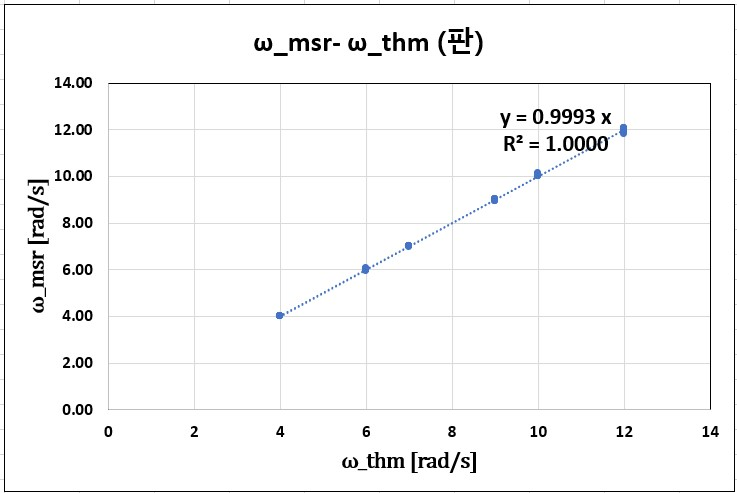
\includegraphics[height=5cm]{images/Experiment(omega_thm-omega_msr)_Plate_Kor.jpg}
%     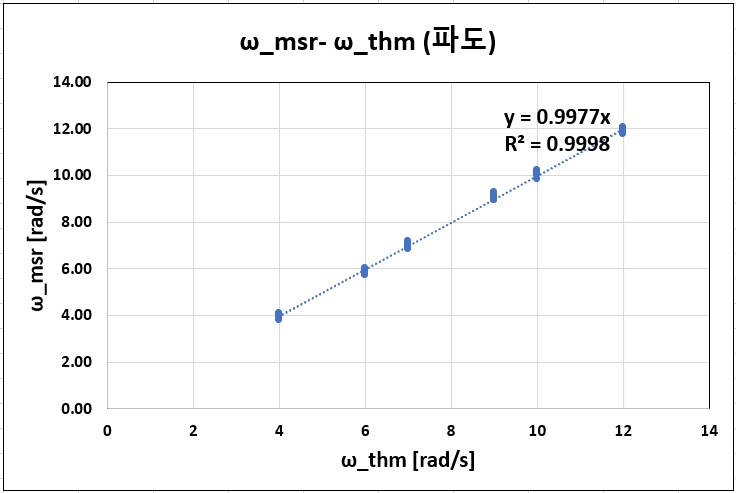
\includegraphics[height=5cm]{images/Experiment(omega_thm-omega_msr)_Wave_Kor.jpg}
%     \caption{측정한 $\omega_{msr}$에 대한 코드의 $\omega_{thm}$ (좌),  $\omega_{msr}$에 대한 측정 진폭 $A_{msr}$ (우) - 검증 실험}
%     \label{ExperimentGraph - 1, 2}
% \end{figure}
%%%%%%%%%%%%%%%%%%%%%%%%%%%%%%%%%%%%%%%%%%%%%%%%%%%%%%%%%%%%%%%%%%%%%%%%%

\begin{figure}[htbp]
    \centering
    \begin{tabular}{ll}
        \begin{filecontents*}{wthm-wwave.dat}
            wthm    wwave
            12  12.03
            12	11.91
            12	11.88
            12	11.96
            12	12.07
            12	12
            12	11.8
            12	12
            12	11.9
            12	11.77
            10	10.2
            10	10.1
            10	10.01
            10	10.07
            10	10.1
            10	10.07
            10	10.09
            10	10.05
            10	10.15
            10	9.84
            9	8.95
            9	9.02
            9	9
            9	9.02
            9	9.15
            9	9.28
            9	9.17
            9	8.94
            9	8.94
            9	8.94
            7	7.16
            7	6.99
            7	6.86
            7	6.99
            7	6.89
            7	6.85
            7	7.06
            7	6.89
            7	6.91
            7	6.9
            6	5.93
            6	5.96
            6	5.97
            6	5.94
            6	6.03
            6	5.73
            6	5.77
            6	5.76
            6	5.94
            6	5.79
            4	3.908
            4	3.984
            4	3.969
            4	3.982
            4	3.978
            4	4.082
            4	4.025
            4	4.051
            4	3.86
            4	3.784            
        \end{filecontents*}
    
        \begin{tikzpicture}[
                %Environment Cfg.
                %font=\bfseries\sffamily,
            ]
            \begin{axis}[
                width=8cm,
                height=8cm,
                at={(0,0)},
                ymin=0,
                ymax=15,
                xmin=0,
                xmax=15,
                grid=both,
                minor tick num =5,
                minor tick style={draw=none},
                minor grid style={thin,color=black!10},
                major grid style={thin,color=black!10},
                %ylabel style={rotate=90},
                ylabel={$\omega_{msr}~\left[\mathrm{rad}/s\right]$},
                xlabel={$\omega_{thm}~\left[\mathrm{rad}/s\right]$},
                tick align=outside,
                axis x line*=middle,
                axis y line*=none,
                xtick={0,2,...,16},
                ytick={0,2,...,16},
                %xlabel style={color=blue!50!cyan},
                %ylabel style={align=center,rotate=-90,color=blue!50!cyan},
                x tick label style={
                    /pgf/number format/assume math mode, font=\scriptsize},
                y tick label style={
                    /pgf/number format/assume math mode, font=\scriptsize},
                legend cell align = {left},
                legend pos = north west,
                legend style={nodes={scale=0.75, transform shape}},
                ]
                \addplot [only marks, 
                    mark size=1pt,
                    mark=o, 
                    %mark options={solid}, 
                    %smooth,
                    ] 
                    table [x=wthm, y=wwave] {wthm-wwave.dat};
                \addlegendentry{$ \omega_{msr}(wave) - \omega_{thm}$}
                \addplot [thick, red] table [y={create col/linear regression={y=wwave}}] {wthm-wwave.dat};
                \addlegendentry{
                    Linear regression: $ \omega_{msr} =
                    \pgfmathprintnumber{\pgfplotstableregressiona}
                    \cdot \omega_{thm}
                    \pgfmathprintnumber[print sign]{\pgfplotstableregressionb}$
                    };

                % \addplot[color=blue!50!cyan,smooth,tension=0.7,very thick] table [x index=0,y index=1,col sep=space] {Aplate-wmsrS.dat};
                % \addplot[color=cyan!50!lime,very thick] coordinates{(0,5)(25,5)};
                % \addplot[color=orange,very thick] coordinates{(0,11)(25,11)};
                % \addplot[color=red!80!orange,very thick] coordinates{(19,24.2)(23,24.2)};
                % \node[text=cyan!50!lime,fill=white,align=center,anchor=west,scale=0.8,inner sep=5pt] at (24.5,5){Base\\ Load};
                % \node[color=orange,fill=white,align=center,anchor=west,scale=0.8,inner sep=5pt] at (24.5,11){Average\\ Load};
                % \node[color=red!80!orange,fill=white,align=center,anchor=west,scale=0.8,inner sep=5pt] at (21.2,24.2){Maxium\\ Load};
            \end{axis}
        \end{tikzpicture}
        
        &
        
        \begin{filecontents}{wthm-wplate.dat}
                    wthm   wPlate
                    12	12.00
                    12	12.04
                    12	12.06
                    12	12.01
                    12	11.81
                    12	12.06
                    12	11.88
                    12	11.98
                    12	11.89
                    12	11.95
                    10	10.00
                    10	10.06
                    10	10.04
                    10	10.05
                    10	9.99
                    10	10.14
                    10	9.99
                    10	10.00
                    10	10.10
                    10	9.99
                    9	9.00
                    9	9.00
                    9	8.98
                    9	8.99
                    9	8.93
                    9	8.95
                    9	8.91
                    9	9.00
                    9	8.99
                    9	9.00
                    7	7.00
                    7	7.00
                    7	7.00
                    7	7.00
                    7	7.00
                    7	6.99
                    7	7.00
                    7	6.99
                    7	7.00
                    7	6.98
                    6	6.00
                    6	6.00
                    6	5.99
                    6	6.01
                    6	5.94
                    6	5.99
                    6	6.00
                    6	6.00
                    6	6.04
                    6	6.05
                    4	4
                    4	4
                    4	4.001
                    4	4.001
                    4	4.001
                    4	4.001
                    4	4
                    4	4
                    4	4.001
                    4	4.001   
            \end{filecontents}
        
            \begin{tikzpicture}[
                    %Environment Cfg.
                    font=\bfseries\sffamily,
                ]
                    \begin{axis}[
                        width=8cm,
                        height=8cm,
                        at={(0,0)},
                        ymin=0,
                        ymax=15,
                        xmin=0,
                        xmax=15,
                        grid=both,
                        minor tick num =5,
                        minor tick style={draw=none},
                        minor grid style={thin,color=black!10},
                        major grid style={thin,color=black!10},
                        %ylabel style={rotate=90},
                        ylabel={$\omega_{msr}~\left[\mathrm{rad}/s\right]$},
                        xlabel={$\omega_{thm}~\left[\mathrm{rad}/s\right]$},
                        tick align=outside,
                        axis x line*=middle,
                        axis y line*=none,
                        xtick={0,2,...,16},
                        ytick={0,2,...,16},
                        %xlabel style={color=blue!50!cyan},
                        %ylabel style={align=center,rotate=-90,color=blue!50!cyan},
                        x tick label style={
                            /pgf/number format/assume math mode}, %, font=\scriptsize
                        y tick label style={
                        /pgf/number format/assume math mode}, %, font=\sf\scriptsize
                        legend cell align = {left},
                        legend pos = north west,
                        legend style={nodes={scale=0.75, transform shape}},
                        ]
                        \addplot [only marks, 
                            mark size=1pt,
                            mark=o, 
                            ]
                            table [x=wthm, y=wPlate] {wthm-wplate.dat};
                        \addplot [thick, red] table [y={create col/linear regression={y=wPlate}}] {wthm-wplate.dat};
                        \addlegendentry{$ \omega_{msr}(plate) - \omega_{thm}$}
                        \addlegendentry{
                            Linear regression: $ \omega_{msr} =
                            \pgfmathprintnumber{\pgfplotstableregressiona}
                            \cdot \omega_{thm}
                            \pgfmathprintnumber[print sign]{\pgfplotstableregressionb}$
                        };

                        % \addplot[color=blue!50!cyan,smooth,tension=0.7,very thick] table [x index=0,y index=1,col sep=space] {Aplate-wmsrS.dat};
                        % \addplot[color=cyan!50!lime,very thick] coordinates{(0,5)(25,5)};
                        % \addplot[color=orange,very thick] coordinates{(0,11)(25,11)};
                        % \addplot[color=red!80!orange,very thick] coordinates{(19,24.2)(23,24.2)};
                        % \node[text=cyan!50!lime,fill=white,align=center,anchor=west,scale=0.8,inner sep=5pt] at (24.5,5){Base\\ Load};
                        % \node[color=orange,fill=white,align=center,anchor=west,scale=0.8,inner sep=5pt] at (24.5,11){Average\\ Load};
                        % \node[color=red!80!orange,fill=white,align=center,anchor=west,scale=0.8,inner sep=5pt] at (21.2,24.2){Maxium\\ Load};
                    \end{axis}
        \end{tikzpicture}
    \end{tabular}
    \begin{tikzpicture} [remember picture, overlay]
        \node at (-14.8, -3.5) {{(a)}};
        \node at (-6.7, -3.5) {{(b)}};
    \end{tikzpicture}
    \caption{$\omega_{msr} - \omega_{thm}$ 그래프- (a) 파도 (b) 조파판}
    \label{Experiment: omega - omega graph}
\end{figure}

그림 \ref{Experiment: omega - omega graph}에서 알 수 있듯이 $\omega$는 코드에서 대입한 값과 판, 파도 모두 같은 값을 띔을 알 수 있다 (두 그래프 모두 선형 관계를 만족하며($R^2 > 0.99$) 그 기울기는 약 1.000이다). 또, 분산 관계식과 식 \ref{eq:5}을 통해 주어진 $\omega$에 대한 $H/S$를 예측할 수 있고 이를 측정값과 비교해보았다.

%%%%%%%%%%%%%%%%%%%%%%%%% 없애버려야 할 엑셀 사진 %%%%%%%%%%%%%%%%%%%%%%%%%
% \begin{figure}[H]
%     \centering
%     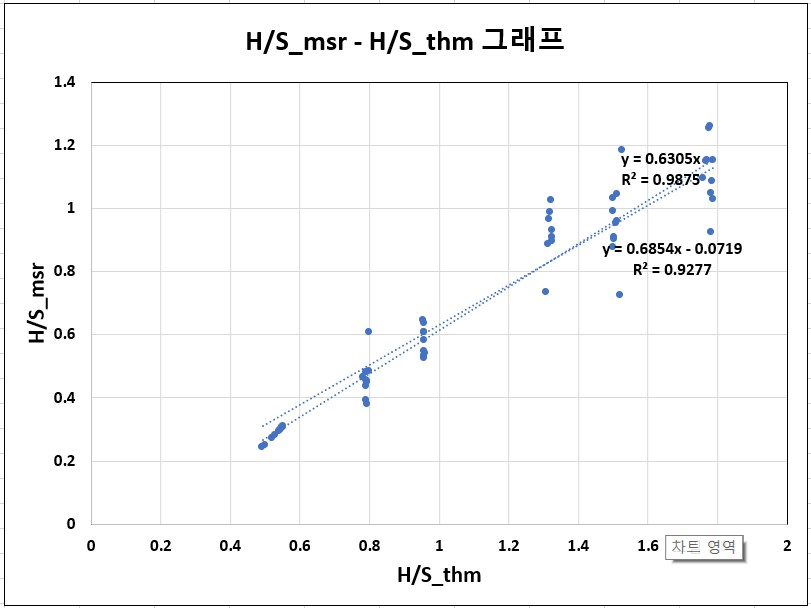
\includegraphics[width=0.70\textwidth]{images/Experiment(H.S_thm-H.S_msr).jpg}
%     \caption{$H/S_{msr} - H/S_{thm}$ 그래프}
%     \label{H/S Graph}
% \end{figure}
%%%%%%%%%%%%%%%%%%%%%%%%%%%%%%%%%%%%%%%%%%%%%%%%%%%%%%%%%%%%%%%%%%%%%%%%%

\begin{figure}[H]
    \centering
        \begin{filecontents}{HSthm-HSmsr.dat}
                HS_thm	HS_msr
                1.781440728	0.925436527
                1.785651376	1.085170025
                1.787735635	1.027713311
                1.782498659	1.045913291
                1.760671425	1.094309648
                1.787735635	1.15104453
                1.768471166	1.150212766
                1.77931432	1.26011236
                1.769571325	1.151819856
                1.776098332	1.252500343
                1.502818971	0.907053163
                1.512879552	1.042827713
                1.509535179	0.952282833
                1.51120852	0.957989748
                1.501134272	0.989520132
                1.526163172	1.182451424
                1.501302842	1.031007752
                1.502482211	0.900403351
                1.519540335	0.724198251
                1.501134272	0.877353529
                1.324569679	0.909190732
                1.324937643	0.929155313
                1.321072373	0.986915888
                1.323465588	1.024621212
                1.313331279	0.887096774
                1.315913161	0.964838394
                1.309086454	0.733436773
                1.326041332	0.895167286
                0.958556795	0.531089978
                0.958906454	0.580898876
                0.959081306	0.608042895
                0.958731617	0.530870712
                0.959081306	0.635545557
                0.956634768	0.607395324
                0.959431056	0.540311804
                0.95646013	0.524718468
                0.958556795	0.547893826
                0.954714602	0.645610278
                0.792888221	0.451327434
                0.792888221	0.377926685
                0.790392394	0.481381958
                0.793981875	0.44980695
                0.783557379	0.464839094
                0.791639619	0.434911243
                0.792419834	0.455155071
                0.79195164	0.393355983
                0.798366989	0.608601216
                0.800094292	0.48515625
                0.492276411	0.242943759
                0.528893957	0.280658651
                0.543862815	0.296883754
                0.553908234	0.308036891
                0.552905492	0.306913997
                0.542089448	0.294936947
                0.546948794	0.300287356
                0.551047756	0.304839279
                0.521368486	0.272679232
                0.499818992	0.25048407                  
            \end{filecontents}
        
            \begin{tikzpicture}[
                    %Environment Cfg.
                    font=\bfseries\sffamily,
                ]
                    \begin{axis}[
                        width=14cm,
                        height=8cm,
                        at={(0,0)},
                        ymin=0,
                        ymax=1.4,
                        xmin=0,
                        xmax=2,
                        grid=both,
                        minor tick num =5,
                        minor tick style={draw=none},
                        minor grid style={thin,color=black!10},
                        major grid style={thin,color=black!10},
                        %ylabel style={rotate=90},
                        ylabel={$H/S_{msr}$},
                        xlabel={$H/S_{thm}$},
                        tick align=outside,
                        axis x line*=middle,
                        axis y line*=none,
                        xtick={0,0.2,...,2},
                        ytick={0,0.2,...,2},
                        %xlabel style={color=blue!50!cyan},
                        %ylabel style={align=center,rotate=-90,color=blue!50!cyan},
                       x tick label style={
                            /pgf/number format/assume math mode, font=\sf\scriptsize},
                        y tick label style={
                            /pgf/number format/assume math mode, font=\sf\scriptsize},
                        legend cell align = {left},
                        legend pos = north west,
                        legend style={nodes={scale=1, transform shape}},
                        ]
                        \addplot[scatter, 
                                only marks, 
                                mark=o,
                                mark size=1.5pt,
                                color=black,
                            ] 
                        table [x=HS_thm, y=HS_msr]{HSthm-HSmsr.dat};    
                        \addplot [thick, red] table [y={create col/linear regression={y=HS_msr}}] {HSthm-HSmsr.dat};
                        %\addlegendentry{$y(x)$}
                        \addlegendentry{
                            Linear regression: $ \omega_{msr} =
                            \pgfmathprintnumber{\pgfplotstableregressiona}
                            \cdot \omega_{thm}
                            \pgfmathprintnumber[print sign]{\pgfplotstableregressionb}$
                        };

                        % \addplot[color=blue!50!cyan,smooth,tension=0.7,very thick] table [x index=0,y index=1,col sep=space] {Aplate-wmsrS.dat};
                        % \addplot[color=cyan!50!lime,very thick] coordinates{(0,5)(25,5)};
                        % \addplot[color=orange,very thick] coordinates{(0,11)(25,11)};
                        % \addplot[color=red!80!orange,very thick] coordinates{(19,24.2)(23,24.2)};
                        % \node[text=cyan!50!lime,fill=white,align=center,anchor=west,scale=0.8,inner sep=5pt] at (24.5,5){Base\\ Load};
                        % \node[color=orange,fill=white,align=center,anchor=west,scale=0.8,inner sep=5pt] at (24.5,11){Average\\ Load};
                        % \node[color=red!80!orange,fill=white,align=center,anchor=west,scale=0.8,inner sep=5pt] at (21.2,24.2){Maxium\\ Load};
                    \end{axis}
        \end{tikzpicture}
    \caption{$H/S_{msr} - H/S_{thm}$ graph}
    \label{H/S graph}
\end{figure}

$H/S$는 선형 관계를 만족한다고 볼 수 있다 (그림 \ref{H/S graph}). 측정값이 구간으로 나타났으나 이는 불확도 내의 값으로 취급할 수 있으며 선형 추세선의 기울기가 $1.000$은 아니지만 선형 추세를 통해 매개변수로부터 $H/S$를 예측할 수 있다.

% \begin{figure}[H]
%     \centering
%     % 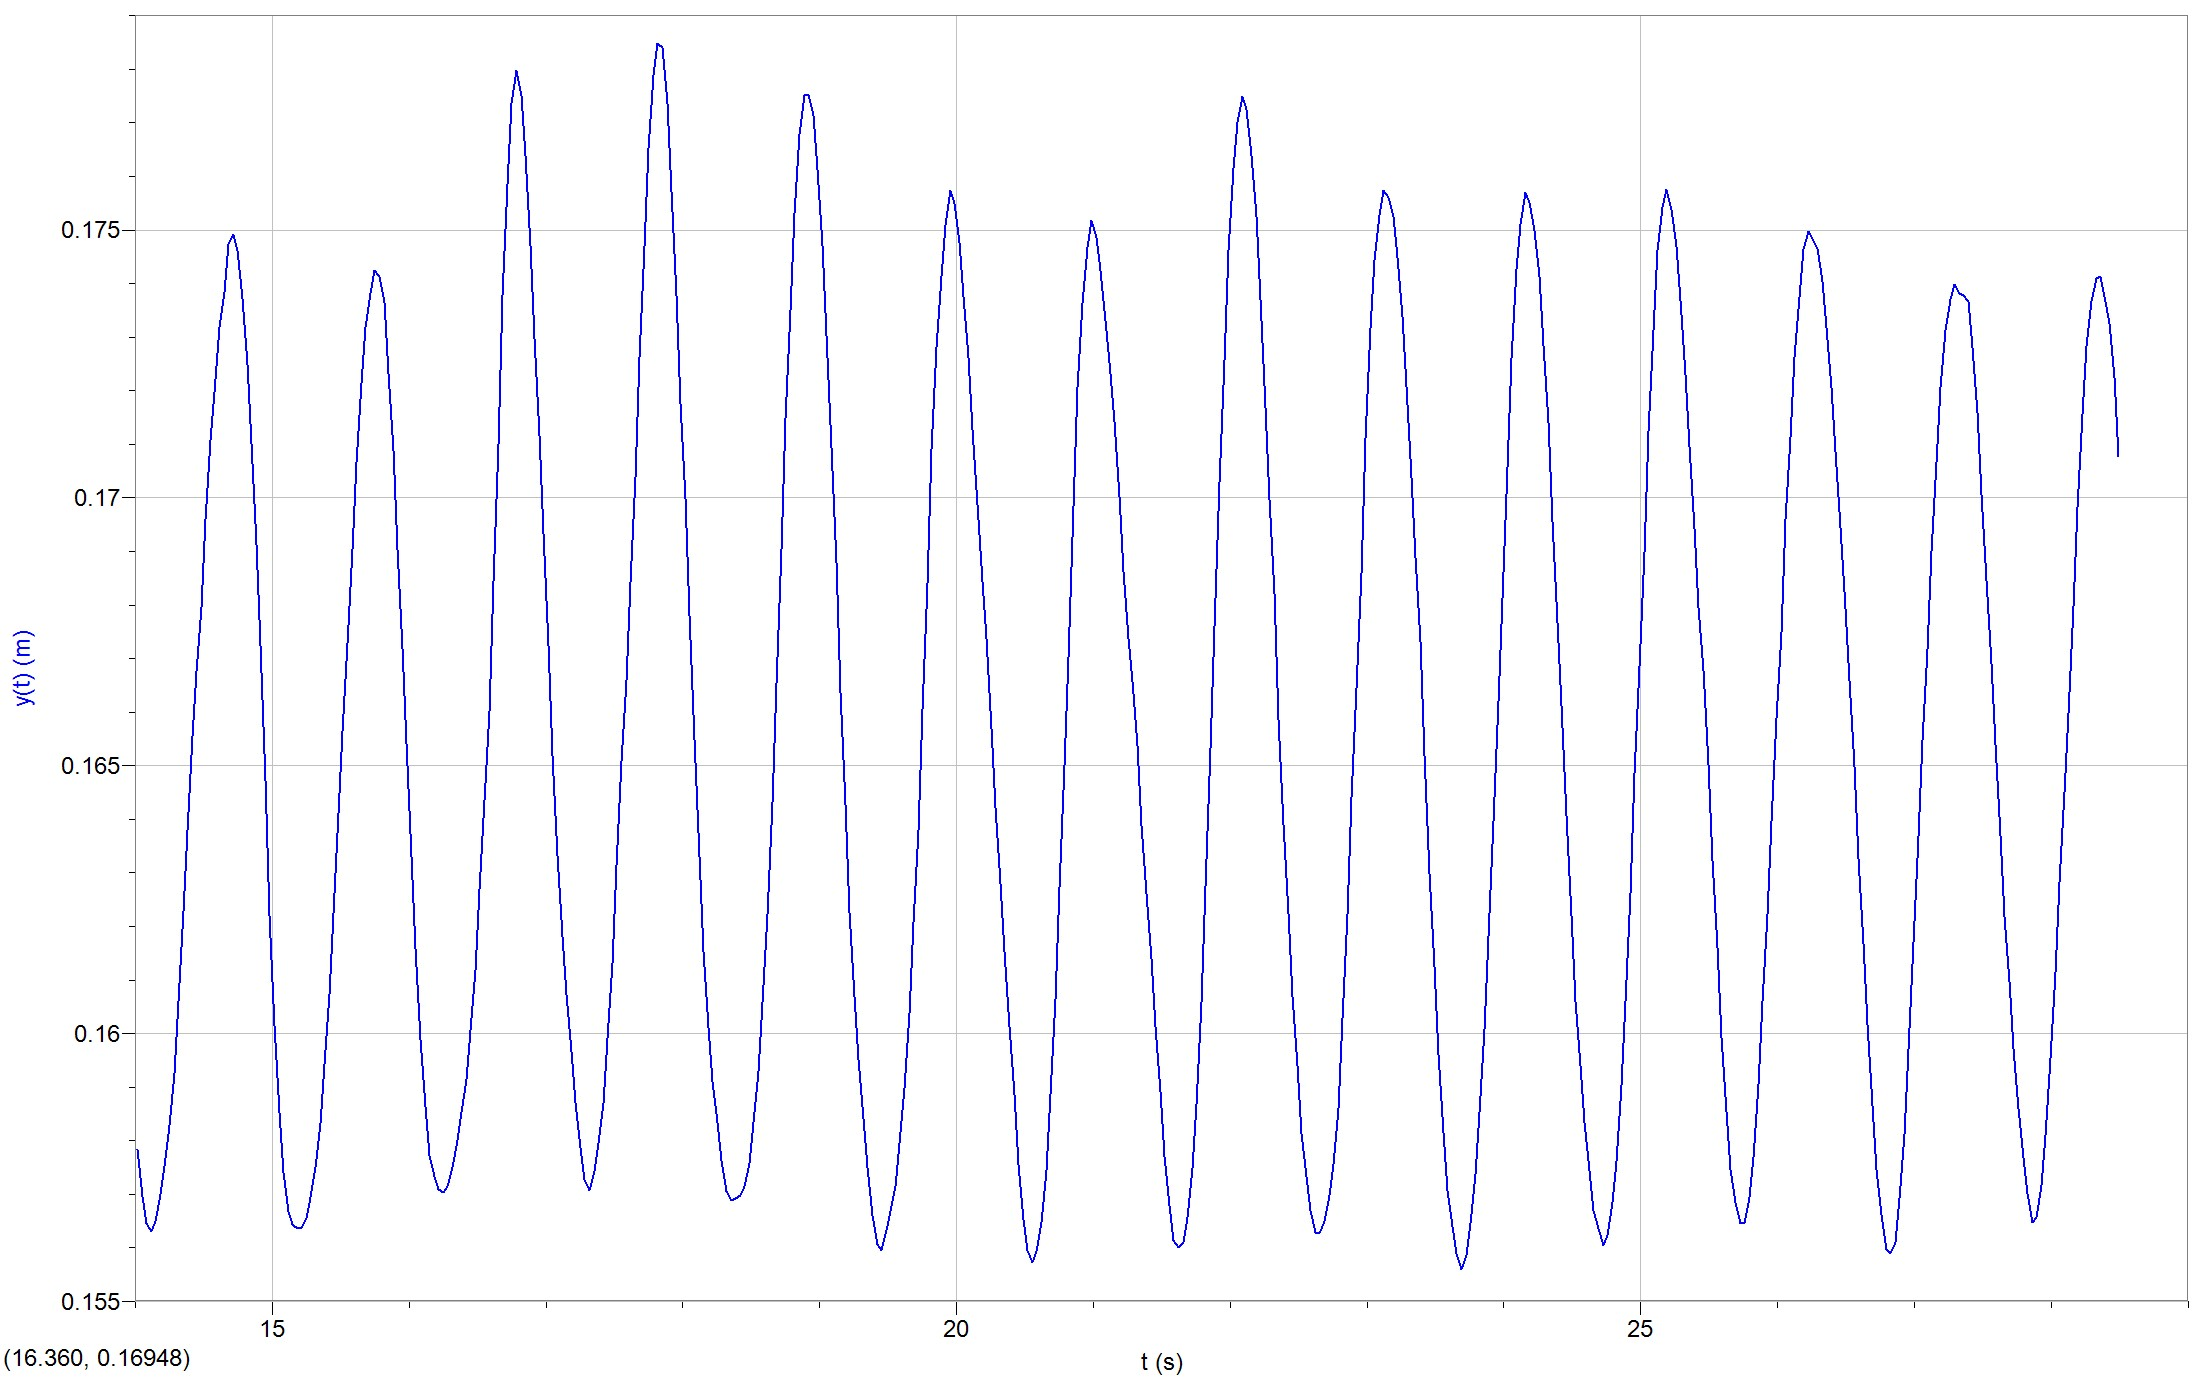
\includegraphics[width=0.70\textwidth]{images/Wave(omega=6,A=2).jpg}
%     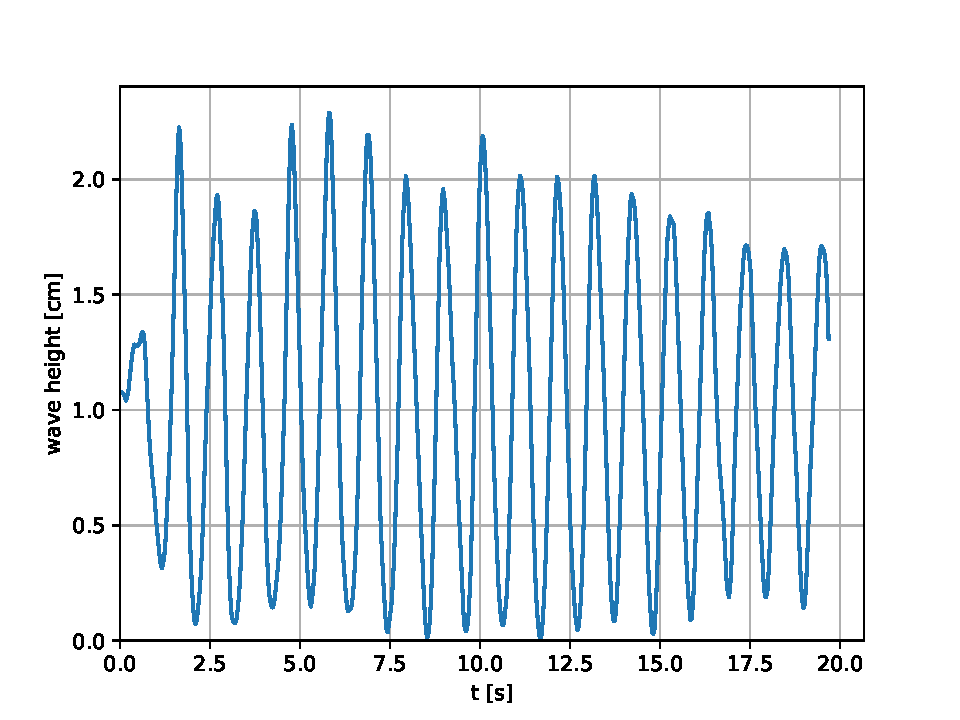
\includegraphics[width=0.70\textwidth]{images/omega=2.00_A=2_wave.pdf}
%     \caption{파형 데이터($A=2\mathrm{~cm},~\omega=6\mathrm{~rad/s}$)}
%     \label{Example Wave Data}
% \end{figure}

% 그림 \ref{Example Wave Data}는 한 sin 파의 예시이다. 코드에서는 $A=2\mathrm{~cm},~\omega=6\mathrm{rad/s}$를 대입하였으며 측정값은 $A=0.9588\mathrm{~cm},~\omega=5.959\mathrm{~rad/s}$이다. 

\subsection{오차 원인}

본 실험에서는 실험 과정에서의 오차, 분석 상의 오차 등 여러 오차가 존재한다. 이는 크게 모터에 의한 것과 파고계 영상 분석에 의한 것으로 나눌 수 있다.

모터의 한계에 의해 $\omega$에 따른 $A$의 한계와 아두이노에서 업로드한 파의 형태에 오차가 생긴다. 최대 각가속도가 판 움직임의 진폭과 오차를 결정한다는 것은 실험을 통해 알 수 있었으며 $\omega = 6$, $A = 5\mathrm{~cm}$의 고정된 상태에서 각가속도만 $30,000\mathrm{~step/s^2}$, $40,000\mathrm{~step/s^2}$, $50,000\mathrm{~step/s^2}$로 바꿔가며 판의 움직임을 분석하였다. 판 움직임을 정렬한 결과가 그림 \ref{fig:diffa}이다. $x$축은 시간이고 $y$축은 판의 변위($\mathrm{~m}$)이고 눈금 한 개의 스케일은 $0.01\mathrm{~m}$이다.

\begin{figure}[H]
    \centering
        \begin{filecontents}{acc.dat}
                t	y_30000	y_40000	y_50000
                0	0.19965	-0.0461	-0.70283
                0.033367	0.88578	0.79731	0.26519
                0.066734	1.41854	1.54643	1.3542
                0.1001	1.78019	2.09436	2.16649
                0.133467	2.10058	2.51832	2.74721
                0.166834	2.42496	2.9166	3.28632
                0.2002	2.65052	3.25279	3.73685
                0.233567	2.69128	3.32493	3.95223
                0.266934	2.69601	3.32011	4.0169
                0.3003	2.68381	3.31722	4.04341
                0.333667	2.53945	3.18505	3.92908
                0.367034	2.24984	2.85109	3.62093
                0.4004	1.94568	2.46075	3.19471
                0.433767	1.6103	2.00279	2.6843
                0.467134	1.14521	1.38601	1.98441
                0.5005	0.55864	0.64207	1.11098
                0.533867	-0.0586	-0.14149	0.16794
                0.567234	-0.68693	-0.94865	-0.8004
                0.6006	-1.16272	-1.669	-1.63958
                0.633967	-1.51151	-2.20274	-2.34206
                0.667334	-1.86959	-2.67197	-3.00563
                0.7007	-2.15706	-3.05802	-3.48397
                0.734067	-2.2686	-3.25109	-3.80335
                0.767434	-2.3295	-3.3759	-4.05893
                0.8008	-2.3925	-3.44363	-4.18022
                0.834167	-2.34221	-3.34345	-4.09689
                0.867534	-2.12824	-3.09611	-3.91013
                0.9009	-1.92868	-2.80851	-3.63691
                0.934267	-1.66742	-2.44389	-3.16259
                0.967634	-1.20691	-1.87777	-2.55154
                1.001	-0.71952	-1.22286	-1.84435
                1.034367	-0.20613	-0.50127	-1.04396
                1.067734	0.42368	0.31501	-0.09588
                1.1011	1.05093	1.12604	0.91296
                1.134467	1.51691	1.75337	1.7925
                1.167834	1.85038	2.20687	2.43867
                1.2012	2.15589	2.58406	3.00982
                1.234567	2.44035	2.96622	3.51607
                1.267934	2.55892	3.18147	3.8099
                1.3013	2.58132	3.1805	3.92574
                1.334667	2.58654	3.18082	3.99092
                1.368034	2.50032	3.12393	3.96888
                1.4014	2.27759	2.85251	3.70347
                1.434767	2.01037	2.44489	3.35212
                1.468134	1.70864	2.02859	2.9192
                1.5015	1.27966	1.48942	2.28589
                1.534867	0.72957	0.7975	1.52725
                1.568234	0.13968	-0.00332	0.65856
                1.6016	-0.46007	-0.82565	-0.34092
                1.634967	-1.00343	-1.61238	-1.27387
                1.668334	-1.39078	-2.12874	-1.98071
                1.7017	-1.73618	-2.63824	-2.67774
                1.735067	-2.05872	-3.06711	-3.25502
                1.768434	-2.2378	-3.33038	-3.59615
                1.8018	-2.28124	-3.46167	-3.88219
                1.835167	-2.35317	-3.55984	-4.08709
                1.868534	-2.34231	-3.52169	-4.05134
                1.9019	-2.18136	-3.3411	-3.88661
                1.935267	-1.96749	-3.06891	-3.67773
                1.968634	-1.71625	-2.72452	-3.26969
                2.002	-1.28602	-2.2191	-2.70558
                2.035367	-0.81728	-1.55728	-2.02746
                2.068734	-0.31872	-0.84745	-1.2709
                2.1021	0.26265	-0.07845	-0.30425
                2.135467	0.9496	0.788	0.72003
                2.168834	1.40154	1.52533	1.62134
                2.2022	1.75468	2.01573	2.30078
                2.235567	2.10147	2.46746	2.94581
                2.268934	2.3967	2.87079	3.47737
                2.3023	2.55238	3.15844	3.81726
                2.335667	2.62076	3.23622	4.00602
                2.369034	2.65914	3.27771	4.14932
                2.4024	2.58367	3.24675	4.15548
                2.435767	2.39857	3.05535	3.94408
                2.469134	2.17446	2.71809	3.62721
                2.5025	1.88444	2.34949	3.25509
                2.535867	1.49925	1.85688	2.65401
                2.569234	1.00332	1.21929	1.93541
                2.6026	0.44518	0.50017	1.14535
                2.635967	-0.19936	-0.3095	0.13966
                2.669334	-0.74776	-1.08519	-0.83255
                2.7027	-1.20231	-1.64584	-1.61405
                2.736067	-1.59977	-2.20759	-2.37864
                2.769434	-1.93983	-2.65238	-3.00176
                2.8028	-2.17932	-2.94288	-3.4264
                2.836167	-2.29458	-3.10488	-3.73815
                2.869534	-2.37942	-3.21108	-3.99138
                2.9029	-2.38288	-3.20642	-4.04015
                2.936267	-2.27697	-3.0282	-3.91074
                2.969634	-2.1216	-2.7839	-3.74705
                3.003	-1.91887	-2.45772	-3.3983
                3.036367	-1.55399	-1.99512	-2.917
                3.069734	-1.07152	-1.35359	-2.28586
                3.1031	-0.64736	-0.69868	-1.56226
                3.136467	-0.07503	0.07567	-0.67443
                3.169834	0.62139	0.96725	0.30019
                3.2032	1.15329	1.72133	1.32913
                3.236567	1.52816	2.28082	2.12527
                3.269934	1.89348	2.70848	2.72048
                3.3033	2.24371	3.18353	3.26412
                3.336667	2.43633	3.40231	3.70057
                3.370034	2.53906	3.47484	3.94051
                3.4034	2.60009	3.55977	4.05245
                3.436767	2.56799	3.57702	4.09095
                3.470134	2.42036	3.37121	3.96946
                3.5035	2.20923	3.07584	3.65483
                3.536867	1.93066	2.78252	3.2648
                3.570234	1.55913	2.26567	2.78462
                3.6036	1.10325	1.61979	2.07279
                3.636967	0.5802	0.97997	1.24147
                3.670334	-0.02334	0.17924	0.34297
                3.7037	-0.65857	-0.75173	-0.64667
                3.737067	-1.17285	-1.37792	-1.55053
                3.770434	-1.56799	-1.91885	-2.26503
                3.8038	-1.90164	-2.46202	-2.94488
                3.837167	-2.23698	-2.85342	-3.50423
                3.870534	-2.44391	-3.05384	-3.83199
                3.9039	-2.49569	-3.19402	-4.0644
                3.937267	-2.51034	-3.29516	-4.2654
                3.970634	-2.5445	-3.24324	-4.26093
                4.004	-2.42687	-3.03	-4.03252
                4.037367	-2.16947	-2.75013	-3.75746
                4.070734	-1.90945	-2.413	-3.36757
                4.1041	-1.51816	-1.933	-2.83599
                4.137467	-1.03935	-1.29424	-2.10184
                4.170834	-0.50818	-0.57231	-1.2709
                4.2042	0.06957	0.31284	-0.26666
                4.237567	0.73165	1.17361	0.75584
                4.270934	1.2455	1.87399	1.6875
                4.3043	1.58747	2.36544	2.40174
                4.337667	1.89112	2.73069	2.95997
                4.371034	2.16959	3.11726	3.35944
                4.4044	2.37204	3.38282	3.71815
                4.437767	2.4319	3.40654	3.89543
                4.471134	2.42094	3.3675	3.95554
                4.5045	2.3439	3.3302	3.92504
                4.537867	2.18696	3.1265	3.74224
                4.571234	1.92323	2.7545	3.39073
                4.6046	1.59431	2.28924	2.94849
                4.637967	1.21345	1.74871	2.39218
                4.671334	0.71115	1.12462	1.6625
                4.7047	0.12966	0.3269	0.79821
                4.738067	-0.47148	-0.51087	-0.16585
                4.771434	-1.05047	-1.27666	-1.12757
                4.8048	-1.49682	-1.80115	-1.92418
                4.838167	-1.82838	-2.27316	-2.58851
                4.871534	-2.17445	-2.71807	-3.17688
                4.9049	-2.43635	-3.04975	-3.62932
                4.938267	-2.48784	-3.21874	-3.86814
                4.971634	-2.51503	-3.29405	-4.06024
                5.005	-2.56856	-3.30492	-4.15906
                5.038367	-2.4869	-3.1784	-4.04501
                5.071734	-2.25169	-2.91066	-3.74639
                5.1051	-2.01171	-2.55853	-3.3832
                5.138467	-1.7465	-2.1082	-2.98582
                5.171834	-1.28108	-1.54368	-2.3775
                5.2052	-0.75679	-0.94807	-1.61234
                5.238567	-0.19342	-0.15545	-0.61791
                5.271934	0.41501	0.72147	0.35113
                5.3053	0.97708	1.50741	1.32609
                5.338667	1.38601	2.09393	2.13243
                5.372034	1.69529	2.46928	2.73626
                5.4054	1.9505	2.84432	3.30207
                5.438767	2.13855	3.19731	3.73049
                5.472134	2.23725	3.34286	4.02161
                5.5055	2.25088	3.2946	4.16939
                5.538867	2.18332	3.24129	4.16521
                5.572234	2.03225	3.17057	4.03556
                5.6056	1.80633	2.85472	3.7849
                5.638967	1.50978	2.36769	3.37659
                5.672334	1.12638	1.89813	2.83644
                5.7057	0.61015	1.3599	2.17771
                5.739067	0.09032	0.56945	1.35831
                5.772434	-0.51844	-0.26237	0.43367
                5.8058	-1.17384	-1.05176	-0.52577
                5.839167	-1.65163	-1.76004	-1.41355
                5.872534	-1.99282	-2.29776	-2.09461
                5.9059	-2.39362	-2.74567	-2.7724
                5.939267	-2.69534	-3.09648	-3.28198
                5.972634	-2.83697	-3.30478	-3.59474
                6.006	-2.97469	-3.43862	-3.80204
                6.039367	-3.04448	-3.47008	-3.97475
                6.072737	-2.96871	-3.40402	-3.96754
                6.106097	-2.80123	-3.19323	-3.7299
                6.139467	-2.578	-2.91812	-3.37793
                6.172837	-2.32669	-2.54115	-3.01313
                6.206197	-2.02032	-2.05056	-2.49922                    
            \end{filecontents}
        
            \begin{tikzpicture}[
                    %Environment Cfg.
                    font=\bfseries\sffamily,
                ]
                    \begin{axis}[
                        width=0.9\textwidth,
                        height=8cm,
                        at={(0,0)},
                        ymin=-4.3,
                        ymax=4.3,
                        xmin=0,
                        xmax=7,
                        grid=both,
                        minor tick num =5,
                        minor tick style={draw=none},
                        minor grid style={thin,color=black!10},
                        major grid style={thin,color=black!10},
                        %ylabel style={rotate=90},
                        ylabel={$y~\left[\mathrm{cm} \right]$},
                        xlabel={$t~\left[\mathrm{s} \right]$},
                        tick align=outside,
                        axis x line*=middle,
                        axis y line*=none,
                        xtick={0, 2, 4, 6, 8},
                        ytick={-4, -2, 0, 2 ,4},
                        %xlabel style={color=blue!50!cyan},
                        %ylabel style={align=center,rotate=-90,color=blue!50!cyan},
                        x tick label style={
                            /pgf/number format/assume math mode, font=\sf\scriptsize,
                            % yshift={-mod(\ticknum,1)*7em}
                            yshift=.5*\axisdefaultheight
                            % yshift = {7em}
                            },
                        y tick label style={
                            /pgf/number format/assume math mode, font=\sf\scriptsize},
                        legend cell align = {left},
                        % legend pos = north east,
                        legend style={at={(1,1)},anchor=north east},
                        legend style={nodes={scale=1.25, transform shape}},
                        ]
                        %\addplot [only marks, mark = *] table [x=t, y_30000, y_40000, y_50000] {acc.dat};
                        \addplot [%only marks, 
                            mark = +,
                            mark size=1.5pt,
                            color=black,
                            ] 
                            table [x=t, y=y_30000] {acc.dat};
                        \addlegendentry{acc = 30000};
                        \addplot [%only marks, 
                            mark = *,
                            mark size=1.5pt,
                            color=black,
                            ] 
                            table [x=t, y=y_40000] {acc.dat};
                        \addlegendentry{acc = 40000};
                        \addplot [%only marks, 
                            mark = o,
                            mark size=1.5pt,
                            color=black,
                            ] 
                            table [x=t, y=y_50000] {acc.dat};
                        \addlegendentry{acc = 50000}; 
                        % \addplot[color=blue!50!cyan,smooth,tension=0.7,very thick] table [x index=0,y index=1,col sep=space] {Aplate-wmsrS.dat};
                        % \addplot[color=cyan!50!lime,very thick] coordinates{(0,5)(25,5)};
                        % \addplot[color=orange,very thick] coordinates{(0,11)(25,11)};
                        % \addplot[color=red!80!orange,very thick] coordinates{(19,24.2)(23,24.2)};
                        % \node[text=cyan!50!lime,fill=white,align=center,anchor=west,scale=0.8,inner sep=5pt] at (24.5,5){Base\\ Load};
                        % \node[color=orange,fill=white,align=center,anchor=west,scale=0.8,inner sep=5pt] at (24.5,11){Average\\ Load};
                        % \node[color=red!80!orange,fill=white,align=center,anchor=west,scale=0.8,inner sep=5pt] at (21.2,24.2){Maxium\\ Load};
                    \end{axis}
        \end{tikzpicture}
    \caption{가속도를 다르게 한 경우의 파고 데이터}
    \label{fig:diffa}
\end{figure}

\begin{table}[H]
    \centering
    \caption{각가속도에 따른 진폭과 오차(RMSE)}
    \begin{tabular}{l|ll}
    \hline
    각가속도$(\mathrm{step/s^{2}})$ & $A (\mathrm{m})$ & RMSE \\
    \hline
    30,000 & 0.02626 & $2.052\times10^{-3}$ \\
    40,000 & 0.03494 & $1.723\times10^{-3}$ \\
    50,000 & 0.04215 & $1.457\times10^{-3}$\\
    \hline
    \end{tabular}%
\end{table}

세 파동 모두 목표한 진폭인 $5\mathrm{~cm}$에 도달하지 못한 이유는 파의 구현에 필요한 각가속도가 $50,000\mathrm{~step/s^2}$보다 크기 때문이라 볼 수 있는데 물의 높이 $15\mathrm{~cm}$를 기준으로 파가 중첩되어 생길 수 있는 최대 물의 높이에서 모터가 탈조나지 않기 위한 조건이 각가속도가 $30,000\mathrm{~step/s^2}$ 이하이므로 스텝모터로는 위의 $A-\omega$ 그래프에서 확인할 수 있는 정상적으로 구현되는 파만 구현 가능하다.

%파도의 높낮이 변화가 극단적인 경우 부표식 파고계의 스티로폼 조각이 물 속에 잠겨버림->그로 인해서 진폭이 이론값보다 작게 나타남

%팽팽하게 위로 늘어났다가 풀리며 작은 마루가 옆에 생겨나는 현상도 관찰됨'

%쇄파 현상으로 인해 부표 위의 표식을 트래킹할 수 없

또, 본 실험에서는 스펀지와 유사한 재질의 포장재를 이용하여 얇은 직사각형판 모양의 부표를 만들어 사용하였다. 위치를 트래킹하여 파고를 측정하였는데 부표의 재질이 스펀지와 비슷하게 구멍이 많이 뚫려있어 파도의 높낮이 변화가 극단적인 경우 잠시 잠기는 현상이 관찰되었다. 이로 인해 진폭이 이론값보다 작게 측정되었으며 부표가 $y$축을 따라서만 이동하지 않기 때문에 오차가 발생한다. 수평 운동을 제어하기 위하여 부표에 두 개의 구멍을 뚫고 실을 통과시켰는데 마찰에 의해 부표가 파도를 따라 움직이는 과정에서 실이 늘어나고 부표가 내려올 때 탄성에 의하여 위로 튀어오르는 오차가 발생한다. 추가적으로, 쇄파 현상이 생기는 경우 부표의 정중앙 표식이 부서지는 파도에 의해 가려져 정확히 같은 지점을 트래킹하는 것이 불가능하다.


\section{결론}

본 연구에서는 연안 환경 모형 실험을 위한 2차원 조파 수조를 제작하였다. 조파수조는 조파기, 소파기, 연안 모형 등으로 구성되며 수조는 길이 $2,000~\mathrm{mm}$, 높이 $400~\mathrm{mm}$, 폭 $300~\mathrm{mm}$의 모듈 3개로 이루어진 $6,000~\mathrm{mm}$ 길이의 구조체이다. 규격에 맞는 모듈을 추가 제작하여 길이 연장이 가능하다. 조파기는 $80~\mathrm{cm}$ 길이의 리니어 액츄에이터에 아크릴 조파판이 장착되어 움직이는 구동부와 틴지 보드와 모터 드라이버로 회로를 조종하는 제어부가 있다. 조파 수조 내부에서 조파판이 물을 밀어내며 파를 생성하며 수조 말단에는 소파기를 두어 파를 소멸한다. 소파기는 다공성 구조를 가진 플라스틱 바구니를 5층으로 쌓았으며 안에 철 수세미를 채워넣어 효율적으로 파를 소멸시킬 수 있도록 하였다. 조파기의 반대편에는 연안 모형이 있으며 현재 길이 $2,000~\mathrm{mm}$, 높이 $200~\mathrm{mm}$로 기울기가 1/10인 경사로를 설치하였고 탈부착이 가능하여 추후 다른 실험을 진행할 때 제거할 수 있다.

조파기는 다양한 규칙파를 만들 수 있으며 코드 상에서 스텝 모터의 각 위치를 직접 대입하여 변화시킨다. 스텝 모터가 $\sin$형 각 변위를 따를 때 진폭과 진동수를 조작할 수 있으며 생성파의 진동수는 입력값과 같지만 파고는 적당한 Calibration을 통하여 찾아야 한다. 본 연구에서는 조파기가 생성한 파의 $H/S$와 이론적인 $H/S$에 대한 근사적인 식을 제시하였으며 조파판과 벽 사이로 물이 새는 등 여러 오차 요인이 존재하여 실험적으로 주어진 파고와 스트로크에 대한 코드의 매개변수 값을 정해야 한다. 구축된 시스템은 여러 기기에 응용할 수 있으며 사용하는 리니어 액츄에이터에 따라서 섬세한 파도 혹은 강력한 파도를 생성할 수 있다.

본 연구에서 제작한 조파 수조는 연안 환경 시뮬레이션이 필요한 연구에 널리 사용될 수 있다. 쓰나미에 의한 피해를 알아보는 연안의 구조물 모형 실험, 파력발전 모형의 효율 비교, 방파제 조적구조의 성능 비교나 선박, 부표 등의 안정성 비교 등의 실험에서 쓰일 수 있다. 현재 본교에서 진동수주형 파력 발전과 관련된 연구가 진행 중이며 조파 수조가 사용될 예정이다.

\section{추후 연구}

\subsection{실험 환경 조성}
조파기와 관련하여 여전히 많은 매개 변수와 조작 변인이 존재한다. $N$, 모터 드라이버의 전류나 스텝 개수 등 다양한 조작 변인을 세워 섬세한 파를 생성할 수 있다. 실험적으로 접근해야하며 시간적 제약으로 인해 제작 및 기본 실험 ($A,~\omega$에 따른 개형 관찰)만 진행하였으나 조파기에 대한 더 나은 이해가 가능하다. 파고계의 위치를 바꿔가면서 조파기와의 거리에 따른 감쇠 효과에 대해 알아볼 수도 있다.

소파기에 대한 연구를 진행할 수도 있는데 현재는 바구니에 수세미를 담은 다공성 구조체를 수조의 양 말단에 두었으나 3D 프린터로 정형화시켜 구멍의 크기나 배치 등에 따른 소파 효과를 확인할 수 있다. 참고문헌에 의하면 다공성 구조가 아닌 일반 벽과 같은 소파기는 표면이 포물면일 때 제일 소파 효과가 크다고 한다.

\subsection{불규칙 파 생성}
조파기의 기본적인 목표는 축소 모형 실험에서 이에 맞는 환경을 조성해주는 것으로 불규칙 파를 생성할 수 있어야 한다. 그 방법으로는 크게 조파판을 바꾸는 방법과 파 생성함수를 바꾸는 방법이 있다. 조파판을 바꾸는 것은 일체형으로 움직이는 조파판을 여러 요소로 나누어 다르게 움직이도록 하는 것이다.

\begin{figure}[htbp]
    \centering
    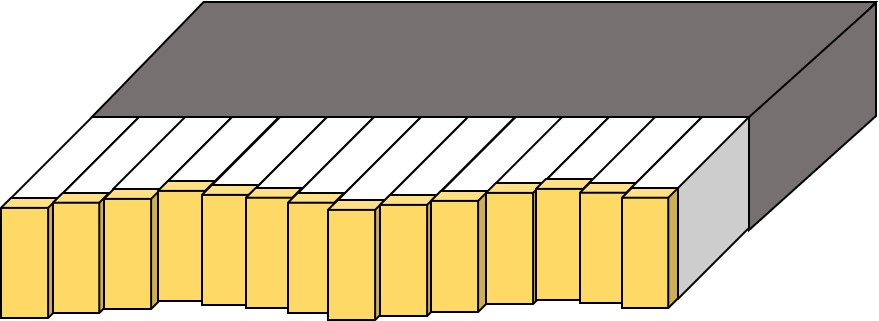
\includegraphics[width=10cm]{images/Wave_Maker(Snake).jpg}
    \caption{3차원 piston형 조파기}
    \label{Snake Wave Maker}
\end{figure}

%사진이 필요함.
3차원 조파 수조로의 확장을 의미하며 조파판을 각 요소로 나누는 것이 유의미하려면 수조가 길고 좁은 것이 아닌 넓은 정사각형 모양이어야 한다. 공간적 제약이 있으며 물을 여러 요소가 밀어내어 snake-like-wave를 발생시킬 수 있다. 현재는 $sin$파만 생성시켰으나 불규칙 파를 생성하는 것이 조파기의 궁극적인 목표이며 piston형 조파기의 판이 여러 조각으로 갈라져 각 요소가 위상차를 두고 움직여야 한다. 그만큼 많은 개수의 모터가 필요하며 구동 방식을 달리 해야할 수도 있다.

\section{부록: Arduino Code for Wave Maker}

\subsection*{move.ino}
\begin{minted}[frame=lines, linenos, fontsize=\scriptsize]
{arduino}
boolean limitCheck(int V){
  if(limitSensorOn()&&V>0){
    rotatecontrol.overrideSpeed(0);
    return false;
  }
  return true;
}
void initializeMotor(){
  int V = 5000;
  while(limitCheck(V)){
    vel(V);
  } vel(0);
  leftEnd = motor.getPosition();
  delay(300);
  while(limitCheck(-V)){
    vel(-V);
  }
  rightEnd = motor.getPosition(); vel(0);
  MID = (leftEnd+rightEnd)/2;
  gotoMiddle();
}
\end{minted}


\subsection*{sin\_wave.ino}
\begin{minted}[frame=lines, linenos, fontsize=\scriptsize]
{arduino}
void sin_set(float k,int a){
  waveset = true;
  A = a; A *= 400; w = k*PI;
   while(motor.getPosition()<MID+A){
    vel(5000);
  } vel(0);
  delay(5000);
  timer = 0; intervalTimer = 0;
}
void sinWave(){
  if(intervalTimer>N){
    intervalTimer = 0;
    float n_speed = (sinmillis(timer+N)-sinmillis(timer))/((float)N/1000);
    vel(n_speed);
  }
}
float sinmillis(float T){
  NUM(0);
  return A*cos(w*T/1000);
}
\end{minted}